\chapter{幂均值 MirrorOPD：目标、镜像更新与方差控制}
\label{ch:proximal-families}

本章研究单教师、每个 prompt 一条 rollout、冻结锚点和 BPO 内层的 MirrorOPD。形状参数 $\kappa$ 改变学生与教师之间的目标分布；插值强度 $\eta$ 决定教师参与程度。推导围绕四个动作组织：构造 target、识别精确镜像目标、拟合 target、控制条件采样误差。前六节给出算法主线及形状选择的结论；后三节给出估计器、高维动力学和适用边界。所有条件分布定理都注明冻结测度、正支持和精确更新要求。

\section{单教师问题与统一条件}
\label{sec:power-setup}
\subsection{冻结锚点、教师与当前学生}

教师分布为 $T(a\mid s)$，本轮冻结学生锚点为 $q_n(a\mid s)$，当前 inner 学生为 $p_{n,j}(a\mid s)=\pi_{\theta_{n,j}}(a\mid s)$。固定一个前缀 $s$ 时省略条件及索引，写成 $T,q,p$。词表 $\mathcal V$ 有限；本章的精确分布定理要求 $q_a,T_a,p_a>0$ 且各自归一化。两个基本概率比为
\begin{equation}
 \rho_a=\frac{T_a}{q_a},\qquad r_a=\log\rho_a,\qquad
 U_\theta(a)=\log\frac{p_\theta(a)}{q_a},\qquad
 C_qh=h-\E_qh.
 \label{eq:power-chapter-ratios}
\end{equation}
对每个 prompt 槽位仅生成一条 $y\sim q_n(\cdot\mid x)$，再冻结所得到的有效前缀及归一化权重，形成经验测度 $\widehat d_n$。一个 batch 可以含 $B$ 个 prompt 槽位；$B$ 不表示同一 prompt 的候选组数。每个前缀可用完整词表求和或辅助 action 抽样来计算损失，辅助 action 不等于新增完整 response。

\begin{center}
\begin{tabular}{lp{108mm}}
\toprule
记号 & 含义与更新时点\\
\midrule
$\kappa\in[0,1]$ & 幂均值 target 的形状；同一理论迭代中固定\\
$0<\eta<1$ & 教师插值强度；也是该 target 的精确 MD 步长\\
$\tau$ & 固定教师目标后可另选的 MD 步长，通常 $0<\tau\le\eta$\\
$\alpha_{\mathrm{opt}}$ & 实际 BPO 参数优化器的步长，与 $\eta,\tau$ 区分\\
$\gamma_j,\xi_j$ & 理想 BPO 的 logit 松弛系数和累计拟合进度\\
$\zeta$ & 辅助 action 提案中教师的混合权重\\
$N,I,M,J$ & outer 预算、每轮 inner 次数、辅助 action 数、保留 head 大小\\
\bottomrule
\end{tabular}
\end{center}

本章统一使用 $\eta$。早期解析图中的 $\lambda$、亲和度 $A$、拟合进度 $\beta$ 和连续时间 $\tau$，分别对应正文的 $\eta,a,\xi,t$。边界 $\eta=1$ 时所有 target 都为 $T$；$\eta=0$ 只用于极限或不更新的参照，不代入含 $1/\eta$ 的 BPO 损失。本轮 $q_n,T,\widehat d_n$ 和教师信号全部停止梯度，学生条件中心在每次 inner 重新计算。外层结束后才将拟合后的学生用作下一轮锚点。

\subsection{目标构造、镜像下降与 BPO 拟合的关系}

幂均值框架中有五个不同角色。重心散度 $D_\kappa$ 定义中间 target $m$；教师目标 $\mathcal J_{\kappa,\eta}$ 解释精确外层 MD；$\KL(p\Vert q)$ 保留负熵 mirror 几何；BPO 用冻结 $q$ 拟合 $m$；教师中心 $K_{\kappa,\eta}$ 将条件监督均值归零。重心问题与 BPO 的最小点是本轮 $m$，教师目标 $\mathcal J$ 的最小点是固定 $T$，KL 正则的最小点是 $q$。$m$ 是向教师目标执行一次 mirror 更新的结果，不是 $\mathcal J$ 的全局最小点；$K$ 在 inner 中则只是冻结中心。

\begin{figure}[H]
 \centering
 \begin{tikzpicture}[every node/.style={font=\small},node distance=13mm]
  \node[draw,rounded corners,align=center,text width=35mm] (source) {本轮冻结分布\\学生 $q_n$、教师 $T$};
  \node[draw,rounded corners,align=center,text width=37mm,right=10mm of source] (target) {幂均值 target $m_n$\\重心 $D_\kappa$；MD 目标 $\mathcal J$};
  \node[draw,rounded corners,align=center,text width=35mm,right=10mm of target] (fit) {BPO 拟合\\当前学生 $p_{n,j}$};
  \node[draw,rounded corners,align=center,text width=35mm,below=of source] (roll) {每个 prompt 一条 rollout\\冻结前缀测度 $\widehat d_n$};
  \node[draw,rounded corners,align=center,text width=37mm,below=of target] (loss) {冻结 $q_n$ 的条件方差\\$\Var_{q_n}[\log(p/m_n)]/(2\eta)$};
  \node[draw,rounded corners,align=center,text width=35mm,below=of fit] (sync) {完成本轮 inner\\同步 $q_{n+1}=p_{n,I}$};
  \draw[->] (source) -- node[above]{$\kappa,\eta$} (target);
  \draw[->] (target) -- node[above]{监督} (fit);
  \draw[->] (source) -- node[right]{$y\sim q_n$} (roll);
  \draw[->] (roll) -- node[above]{权重} (loss);
  \draw[->] (loss) -- (fit);
  \draw[->] (fit) -- (sync);
 \end{tikzpicture}
 \caption{单教师、单 rollout 的主线。中间分布是监督 target；response 仍由学生锚点生成。精确求到 target 与神经网络有限步拟合分别承担外层和内层的数学条件。}
 \label{fig:divergence-map-roles}
\end{figure}

\subsection{小插值强度与重尾监督的区别}

对固定随机向量 $X$，$\Var(\eta X)=\eta^2\Var(X)$，其均值也缩小为 $\eta\E X$。若均值非零，相对噪声 $\Var(\eta X)/\|\eta\E X\|^2$ 不变。当前 BPO 损失带 $1/\eta$，其几何端点起始下降方向是 $\E_q[(C_qr)\psi_q]$，不会随 $\eta$ 整体缩小。减小教师参与程度与压制极端概率比是不同操作。

取二元词表 $q=(v,1-v)$、$T_\epsilon=(\epsilon,1-\epsilon)$，其中 $0<v<1$、$v\ne1/2$。对第一个 categorical logit，$\psi_q(1)=1-v$、$\psi_q(2)=-v$。令
\begin{equation}
 r_1=\log(\epsilon/v),\qquad r_2=\log[(1-\epsilon)/(1-v)],\qquad D=r_1-r_2.
\end{equation}
精确条件中心化给出 $C_qr(1)=(1-v)D$、$C_qr(2)=-vD$。单 action 梯度 $X=(C_qr)\psi_q$ 分别取 $(1-v)^2D$、$v^2D$，因此
\begin{align}
 \E_qX&=v(1-v)D,\\
 \Var_qX&=v(1-v)(1-2v)^2D^2.
 \label{eq:proximal-binary-variance}
\end{align}
$D=\log\epsilon+O(1)$，所以 $\Var_qX\to\infty$，任意固定 $\eta>0$ 也不能使 $\eta^2\Var_qX$ 具有分布无关界。这个反例已有精确 baseline 和有界 score。$v=1/2$ 时中心化后的二元 score 梯度恰为常数，必须用非对称的 $q$ 才能证明梯度方差发散。

本章的改进方向是改变冻结教师信号的形状，使负尾部饱和，同时保留局部教师差异的尺度。后续要分别证明固定正 $\eta$ 下的界、$\eta\to0$ 的统一界、残差趋零的噪声界，以及完整参数梯度所需的 score 条件。


\section{幂均值目标与散度重心}
\label{sec:proximal-barycenters}
\subsection{$f$ 散度、KL 端点与四种优化对象}
\label{sec:proximal-divergence-map}

本小节先固定散度方向，再区分定义 target 的重心目标、教师中心、BPO 拟合损失和 mirror 正则。后续全部推导在同一个有限词表上进行，分布严格为正且归一化。KL 本身属于 $f$ 散度；引入 $\kappa$ 是把 KL 端点扩展成一个散度族。这里仍使用 $\lambda$ 表示插值强度；在单教师 BPO 小节中改记为 $\eta=\lambda$。

\subsubsection{生成函数与散度方向}

对凸函数 $g:(0,\infty)\to\mathbb R$、$g(1)=0$，定义 Csisz\'ar $f$ 散度
\begin{equation}
 D_g(P\Vert Q)=\sum_a Q_a g(P_a/Q_a).
 \label{eq:divergence-map-csiszar}
\end{equation}
其中采样或求和参照分布是第二个自变量 $Q$。加上任意线性项 $c(x-1)$ 不改变散度，因为 $\sum Q(P/Q-1)=0$。下面采用 $g(1)=g'(1)=0$ 的规范化生成函数；规范化不改变 KL 方向。

\begin{theorem}[幂散度的 $f$ 表示、对偶与 KL 端点]
\label{thm:divergence-map-power}
设 $0<\kappa<1$，定义
\begin{equation}
 g_\kappa(x)=\frac{\kappa x+1-\kappa-x^\kappa}{\kappa(1-\kappa)}.
 \label{eq:divergence-map-power-generator}
\end{equation}
则 $g_\kappa(1)=g_\kappa'(1)=0$、$g_\kappa''(x)=x^{\kappa-2}>0$，且
\begin{equation}
 D_{g_\kappa}(P\Vert Q)
 =\frac{1-\sum_a P_a^\kappa Q_a^{1-\kappa}}{\kappa(1-\kappa)}
 =D_\kappa(P\Vert Q).
\end{equation}
生成函数的连续端点为
\begin{align}
 g_0(x)&=x-1-\log x,&D_0(P\Vert Q)&=\KL(Q\Vert P),\\
 g_1(x)&=x\log x-x+1,&D_1(P\Vert Q)&=\KL(P\Vert Q).
 \label{eq:divergence-map-kl-endpoints}
\end{align}
交换分布与交换形状满足
\begin{equation}
 D_\kappa(P\Vert Q)=D_{1-\kappa}(Q\Vert P).
 \label{eq:divergence-map-duality}
\end{equation}
采用 $H^2(P,Q)=\sum_a(\sqrt{P_a}-\sqrt{Q_a})^2$ 时，$D_{1/2}=2H^2$。因此两个 KL 方向是同一幂散度族的端点，平方根点是对称的 Hellinger 散度。
\end{theorem}

\begin{proof}
直接微分得到 $g_\kappa'=(1-x^{\kappa-1})/(1-\kappa)$ 与 $g_\kappa''=x^{\kappa-2}$。求和时两个线性部分贡献 $\kappa\sum P+(1-\kappa)\sum Q=1$，幂部分贡献 $\sum P^\kappa Q^{1-\kappa}$，得到散度表示。严格凸性和 Jensen 不等式给出非负性；等号要求所有 $P_a/Q_a$ 相同，归一化后即 $P=Q$。

令 $\ell=\log x$。当 $\kappa\to0$，$x^\kappa=1+\kappa\ell+O(\kappa^2)$，故分子为 $\kappa(x-1-\ell)+O(\kappa^2)$，分母为 $\kappa+O(\kappa^2)$。当 $\kappa=1-\epsilon\to1$，$x^\kappa=x-\epsilon x\ell+O(\epsilon^2)$，分子为 $\epsilon(x\ell-x+1)+O(\epsilon^2)$，分母为 $\epsilon+O(\epsilon^2)$。有限词表和正支持允许逐项取极限。相应求和分别是
\begin{align}
 \sum_aQ_a g_0(P_a/Q_a)
 &=\sum_a(P_a-Q_a)-\sum_aQ_a\log(P_a/Q_a)=\KL(Q\Vert P),\\
 \sum_aQ_a g_1(P_a/Q_a)
 &=\sum_aP_a\log(P_a/Q_a)-\sum_a(P_a-Q_a)=\KL(P\Vert Q).
\end{align}
另外 $xg_{1-\kappa}(1/x)=g_\kappa(x)$，代入定义即得交换对偶。$\kappa=1/2$ 时
\begin{equation}
 D_{1/2}=4\left(1-\sum_a\sqrt{P_aQ_a}\right)
 =2\sum_a(\sqrt{P_a}-\sqrt{Q_a})^2.
\end{equation}
\end{proof}

这里的 reverse/forward 以 student 为相对于 teacher 的方向：$D_0(T\Vert p)=\KL(p\Vert T)$，$D_1(T\Vert p)=\KL(T\Vert p)$。同一个有序表达式 $D_g(T\Vert p)$ 可以包含这两种 KL；生成函数决定方向，不能只看括号中的分布顺序。

两个端点对应的加权优化问题为
\begin{align}
 F_0(p)&=(1-\eta)\KL(p\Vert q)+\eta\KL(p\Vert T),\\
 F_1(p)&=(1-\eta)\KL(q\Vert p)+\eta\KL(T\Vert p).
 \label{eq:divergence-map-barycenter-endpoints}
\end{align}
它们的唯一解分别是 $m_0\propto q^{1-\eta}T^\eta$ 与 $m_1=(1-\eta)q+\eta T$。中间形状由 $(1-\eta)D_\kappa(q\Vert p)+\eta D_\kappa(T\Vert p)$ 定义，其重心和精确超额损失在后文证明。

中间生成函数也不同于两个 KL 生成函数的固定线性组合。若存在仅依赖 $\kappa$ 的系数 $a,b$，使规范化生成函数满足 $g_\kappa=ag_0+bg_1$，则二阶导数强制
\begin{equation}
 x^{\kappa-2}=a/x^2+b/x,\qquad x^\kappa=a+bx.
\end{equation}
当 $0<\kappa<1$ 时左边的二阶导数为 $\kappa(\kappa-1)x^{\kappa-2}<0$，右边为零，不能对所有 $x>0$ 成立。这是通过生成函数的曲率连续改变散度，不能用 KL 权重插值替代。

\subsubsection{教师中心属于另一个两参数散度族}

为与单教师 BPO 保持一致，记 $\rho=T/q$、$0<\eta<1$，并定义
\begin{equation}
 A_{\kappa,\eta}(x)=\begin{cases}
 \log x,&\kappa=0,\\
 (\kappa\eta)^{-1}\log(1-\eta+\eta x^\kappa),&\kappa>0.
 \end{cases}
\end{equation}
这里 $A$ 的自变量是概率比 $x$；对 log-ratio 求导时须另作链式变换。教师中心 $K_{\kappa,\eta}=-\E_qA_{\kappa,\eta}(\rho)$ 的生成函数是
\begin{equation}
 \phi_{\kappa,\eta}(x)=x-1-A_{\kappa,\eta}(x),\qquad
 K_{\kappa,\eta}=D_{\phi_{\kappa,\eta}}(T\Vert q).
 \label{eq:divergence-map-center-family}
\end{equation}
因为 $A'(x)=x^{\kappa-1}/(1-\eta+\eta x^\kappa)$，有
\begin{equation}
 \phi''(x)=\frac{x^{\kappa-2}[(1-\kappa)(1-\eta)+\eta x^\kappa]}
 {(1-\eta+\eta x^\kappa)^2}>0.
\end{equation}
$\phi(1)=\phi'(1)=0$，所以它也是凸 $f$ 散度。其端点却是
\begin{align}
 K_{0,\eta}&=\KL(q\Vert T),\\
 K_{1,\eta}&=\eta^{-1}\KL\big(q\Vert(1-\eta)q+\eta T\big),\\
 K_{\kappa,1}&=\KL(q\Vert T).
 \label{eq:divergence-map-center-endpoints}
\end{align}
因此 $K$ 的算术端点是对混合 target 的 reverse KL，不能把 $D_1(T\Vert q)$ 的 forward KL 端点搬到 $K_{1,\eta}$ 上。

两族的准确联系出现在小插值强度极限。对固定正支持分布，令 $\eta\to0$，则
\begin{align}
 A_{\kappa,\eta}(x)&=\frac{x^\kappa-1}{\kappa}+O(\eta),\\
 \phi_{\kappa,\eta}(x)&\longrightarrow
 x-1-\frac{x^\kappa-1}{\kappa}=(1-\kappa)g_\kappa(x),\\
 K_{\kappa,\eta}&\longrightarrow(1-\kappa)D_\kappa(T\Vert q),
 \qquad 0<\kappa<1.
 \label{eq:divergence-map-center-limit}
\end{align}
平方根点满足 $K_{1/2,\eta}\to H^2(q,T)$，而 $D_{1/2}(T\Vert q)=2H^2(q,T)$。在 $\kappa=1$ 处，令 $\delta=\rho-1$，有限词表 Taylor 展开进一步给出
\begin{equation}
 K_{1,\eta}=\frac\eta2\E_q\delta^2+O(\eta^2)
 =\frac\eta2\chi^2(T\Vert q)+O(\eta^2)\longrightarrow0.
\end{equation}
这个零极限与 $D_1(T\Vert q)=\KL(T\Vert q)$ 一般非零形成直接区别。中心的界、方差及估计方法继续见第~\ref{sec:proximal-teacher-center}~小节。

\subsubsection{BPO 是带冻结测度的拟合损失}

对冻结 $q,m$，BPO population 损失是
\begin{equation}
 \mathcal L_{\mathrm{BPO}}(p;m,q)
 =\frac1{2\eta}\Var_q\!\left[\log\frac p m\right].
 \label{eq:divergence-map-bpo-loss}
\end{equation}
它一般不能写成仅以 $(p,m)$ 为自变量的 $D_g(p\Vert m)$。取二元词表，固定 $p,m$ 且 $\ell_1=\log(p_1/m_1)\ne\ell_2=\log(p_2/m_2)$，则
\begin{equation}
 \mathcal L_{\mathrm{BPO}}=\frac{q_1(1-q_1)}{2\eta}(\ell_1-\ell_2)^2.
\end{equation}
改变第三个分布 $q$ 会改变损失，任何固定生成函数的 $D_g(p\Vert m)$ 都不随 $q$ 改变。完整支持下，BPO 与 target 散度共享唯一零点 $p=m$，这一事实不意味着损失、曲率或有限步轨迹相同。

取切向扰动 $p=m+v$、$\sum_av_a=0$，并令全部 $v_a/m_a$ 一致趋零。展开 $\log(1+v_a/m_a)$ 得到
\begin{equation}
 \mathcal L_{\mathrm{BPO}}(m+v;m,q)
 =\frac1{2\eta}\left\{\sum_aq_a\frac{v_a^2}{m_a^2}
 -\left(\sum_aq_a\frac{v_a}{m_a}\right)^2\right\}
 +O\!\left(\max_a|v_a/m_a|^3\right).
\end{equation}
若 $q=m$，一次均值为 $\sum v=0$，二阶项恢复 $\sum v_a^2/m_a$ 的 Fisher 度量，另带 $1/\eta$。一般冻结 $q\ne m$ 时，BPO 的局部度量与 target 上的 Fisher 度量不同。若使用独立 logits $z$，则 $C_q\log(p/m)=C_q(z-\log m)$，全局 Hessian 为 $[\operatorname{diag}(q)-qq^\top]/\eta$，与 $\kappa$ 无关。

\begin{figure}[htbp]
 \centering
 \begin{tikzpicture}[every node/.style={font=\small},node distance=14mm]
  \node[draw,rounded corners,align=center,text width=47mm] (bary) {重心问题\\$(1-\eta)D_\kappa(q\Vert p)+\eta D_\kappa(T\Vert p)$};
  \node[draw,rounded corners,align=center,text width=42mm,right=16mm of bary] (target) {归一化幂均值\\$m\propto[(1-\eta)q^\kappa+\eta T^\kappa]^{1/\kappa}$};
  \node[draw,rounded corners,align=center,text width=47mm,below=of bary] (mirror) {熵镜像子问题\\$\max_p\{\E_pA-\eta^{-1}\KL(p\Vert q)\}$};
  \node[draw,rounded corners,align=center,text width=42mm,below=of target] (fit) {BPO 内层拟合\\$\Var_q[\log(p/m)]/(2\eta)$};
  \node[draw,rounded corners,align=center,text width=47mm,below=of mirror] (center) {教师中心\\$K=-\E_q A=D_\phi(T\Vert q)$};
  \draw[->] (bary) -- node[above]{最优解} (target);
  \draw[->] (mirror) -- node[above,sloped]{精确解} (target);
  \draw[->] (target) -- node[right]{冻结监督} (fit);
  \draw[->] (center) -- node[right,align=center]{条件均值\\零化系数} (fit);
 \end{tikzpicture}
 \caption{同一 target 的不同数学表示。$D_\kappa$ 定义重心，$D_\phi$ 给出教师中心，BPO 使用冻结 $q$ 拟合 target，KL 正则决定 entropy mirror 几何。四者共享一些恒等式，承担的优化角色不同。固定 $(\kappa,\eta)$ 时 mirror 信号还能积分成一个独立于 anchor 的新目标，见第~\ref{sec:proximal-md-objective}~小节。}
 \label{fig:divergence-map-roles}
\end{figure}

幂均值重心的超额损失和外层动力学刻画理想条件优化。分布 $q,t$ 位于同一有限词表，严格为正且各自归一化。固定 $\kappa\in[0,1]$ 与 $\lambda\in(0,1)$。每个 prefix 独立推导，教师在外层更新中固定。这里的精确分布更新不包含神经网络投影和 prefix 测度变化。幂均值重心属于已有的 $\alpha$-integration 理论\footnote{Shun-ichi Amari. Integration of Stochastic Models by Minimizing $\alpha$-Divergence. Neural Computation 19(10), 2007, pp. 2780--2796. \url{https://doi.org/10.1162/neco.2007.19.10.2780}. 本节分别证明重心、自然梯度流、escort 动力学及矩阶数，不据此宣称研究新颖性。}；这些精确性质分别与 MirrorOPD 的目标、拟合误差和方差问题关联。

\subsection{幂均值目标与两个端点}

对 $0<\kappa\le1$ 定义
\begin{equation}
 h_a=[(1-\lambda)q_a^\kappa+\lambda t_a^\kappa]^{1/\kappa},\quad
 Z=\sum_ah_a,\quad m_a=h_a/Z.
 \label{eq:proximal-power-target}
\end{equation}
当 $\kappa\to0$，$q_a^\kappa=1+\kappa\log q_a+O(\kappa^2)$，且 $\log(1+x)=x+O(x^2)$，所以
\begin{equation}
 \lim_{\kappa\to0}\log h_a=(1-\lambda)\log q_a+\lambda\log t_a.
\end{equation}
$\kappa=0$ 因此是几何 target $m_a\propto q_a^{1-\lambda}t_a^\lambda$；$\kappa=1$ 是算术 target $m=(1-\lambda)q+\lambda t$。$\kappa=1/2$ 为平方根 target
\begin{equation}
 m_a=\frac{[(1-\lambda)\sqrt{q_a}+\lambda\sqrt{t_a}]^2}
 {(1-\lambda)^2+\lambda^2+2\lambda(1-\lambda)A},\qquad
 A=\sum_a\sqrt{q_at_a}.
 \label{eq:proximal-square-root}
\end{equation}
$A$ 是 Bhattacharyya 系数，$\arccos A$ 是平方根单位球上的夹角，Fisher--Rao 距离为 $2\arccos A$。平方根 target 沿该球面上的短弧移动，$\lambda$ 通常不是弧长参数\footnote{Mitsuhiro Itoh, Hiroyasu Satoh. Information geometry of the space of probability measures and barycenter maps. arXiv:2208.11861, 2022. \url{https://arxiv.org/html/2208.11861}.}。

由幂均值不等式，$h_a\le(1-\lambda)q_a+\lambda t_a$，因此 $Z\le1$。对 $r=1/\kappa\ge1$，$(x+y)^r\ge x^r+y^r$，又有
\begin{equation}
 h_a\ge(1-\lambda)^{1/\kappa}q_a+\lambda^{1/\kappa}t_a,
 \qquad
 (1-\lambda)^{1/\kappa}+\lambda^{1/\kappa}\le Z\le1.
\end{equation}
归一化常数受控，但它一般不等于一；后续推导必须保留它。

记 $r=\log(t/q)$，与这个 target 对应的未归一化冻结信号为
\begin{equation}
 f_{\kappa,\lambda}(r)=\frac1\kappa\log(1-\lambda+\lambda e^{\kappa r}),\qquad
 f_{0,\lambda}(r)=\lambda r.
 \label{eq:proximal-power-signal}
\end{equation}
它满足 $qe^f=h$、$m\propto qe^f$。因此保留 KL mirror 正则并令其系数为一，就能表示全部幂均值 target；重心散度、拟合损失与冻结信号仍是三个不同的数学对象。

\begin{figure}[htbp]
 \centering
 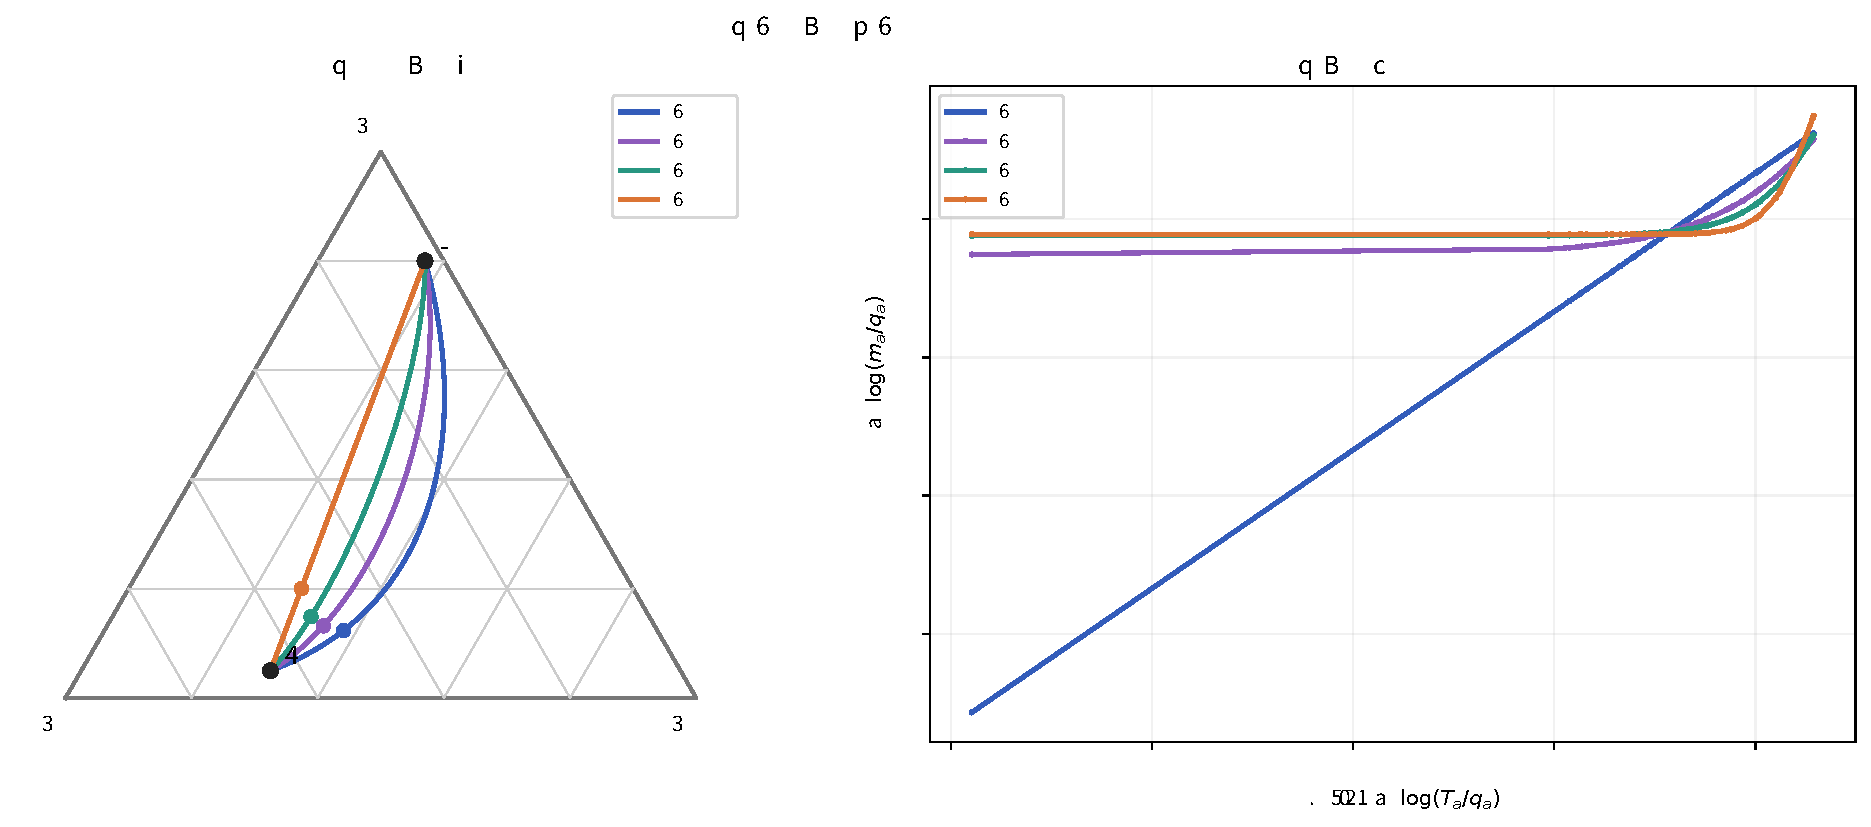
\includegraphics[width=\textwidth]{../../results/proximal-family-geometry/geometry.pdf}
 \caption{幂均值 target 的概率路径与 token log-ratio。左图圆点均为 $\lambda=0.2$；右图以 64 维概率向量展示同一族。形状参数改变高维路径和尾部，而不是仅改变移动距离。}
\end{figure}

\subsection{重心唯一性与超额损失的精确分解}

对 $0<\kappa<1$ 定义
\begin{equation}
 D_\kappa(u\Vert p)
 =\frac{1-\sum_au_a^\kappa p_a^{1-\kappa}}{\kappa(1-\kappa)}.
 \label{eq:proximal-power-divergence}
\end{equation}
Hölder 不等式保证非负，完整支持下等号仅在 $u=p$ 成立。端点由展开给出：当 $\kappa\to0$，$\sum p_a\exp(\kappa\log(u_a/p_a))=1-\kappa\KL(p\Vert u)+O(\kappa^2)$；当 $\kappa=1-\delta\to1$，$\sum u_a\exp(\delta\log(p_a/u_a))=1-\delta\KL(u\Vert p)+O(\delta^2)$。所以
\begin{equation}
 D_0(u\Vert p)=\KL(p\Vert u),\qquad D_1(u\Vert p)=\KL(u\Vert p).
\end{equation}
这固定了本节的 KL 方向，不用不同文献的 $\alpha$ 记号替代定义。

\begin{theorem}[幂均值重心与精确目标误差]
\label{thm:proximal-barycenter-gap}
对 $0<\kappa<1$，令
\begin{equation}
 F(p)=(1-\lambda)D_\kappa(q\Vert p)+\lambda D_\kappa(t\Vert p).
 \label{eq:proximal-divergence-barycenter}
\end{equation}
其唯一最小点是式~\eqref{eq:proximal-power-target} 的 $m$。对任意 $p$ 有
\begin{equation}
 F(p)=\frac{1-Z^\kappa}{\kappa(1-\kappa)}+Z^\kappa D_\kappa(m\Vert p),\qquad
 F(p)-F(m)=Z^\kappa D_\kappa(m\Vert p).
 \label{eq:proximal-gap-identity}
\end{equation}
端点 $\kappa=0,1$ 的超额损失分别为 $\KL(p\Vert m)$ 与 $\KL(m\Vert p)$。
\end{theorem}

\begin{proof}
令 $S_a=(1-\lambda)q_a^\kappa+\lambda t_a^\kappa$。目标写成 $F(p)=(1-\sum_aS_ap_a^{1-\kappa})/[\kappa(1-\kappa)]$。在 $\sum p_a=1$ 约束下，一阶条件为
\begin{equation}
 -\frac{S_a}{\kappa}p_a^{-\kappa}+\nu=0,
 \qquad p_a=(S_a/(\kappa\nu))^{1/\kappa}.
\end{equation}
归一化得到 $m$。目标的概率坐标 Hessian 为 $\operatorname{diag}(S_ap_a^{-\kappa-1})\succ0$，故内点解唯一。由 $S_a=Z^\kappa m_a^\kappa$，直接代入可得
\begin{align}
 F(p)
 &=\frac{1-Z^\kappa\sum_am_a^\kappa p_a^{1-\kappa}}{\kappa(1-\kappa)}\\
 &=\frac{1-Z^\kappa}{\kappa(1-\kappa)}
 +Z^\kappa\frac{1-\sum_am_a^\kappa p_a^{1-\kappa}}{\kappa(1-\kappa)}.
\end{align}
$p=m$ 时散度为零，得精确分解。$\kappa=0$ 时加权 reverse KL 展开为 $\KL(p\Vert m)-\log Z_0$；$\kappa=1$ 时加权 forward KL 展开为 $\KL(m\Vert p)+(1-\lambda)\KL(q\Vert m)+\lambda\KL(t\Vert m)$，其中 $Z_0=\sum q^{1-\lambda}t^\lambda$。端点的超额损失结论随之成立。\hfill$\square$
\end{proof}

定理把“相同 target”加强成了“原重心问题的超额损失与拟合散度精确成比例”。它也给出有限 inner 阶段适合验收的误差：若原问题优化误差为 $\delta$，则 $D_\kappa(m\Vert p)=\delta/Z^\kappa$。MDPO 使用的 $\KL(p\Vert m)$ 与它只有在 $\kappa=0$ 时完全相同；一般 $\kappa$ 下不能仅凭相同最小点替换有限步进展保证。

\subsection{共同的局部 Fisher 曲率与多教师扩展}

取 $p=u+\delta$、$\sum_a\delta_a=0$，并令 $\max_a|\delta_a/u_a|\to0$。逐项展开得到
\begin{equation}
 u_a^\kappa(u_a+\delta_a)^{1-\kappa}
 =u_a+(1-\kappa)\delta_a-\frac{\kappa(1-\kappa)}2\frac{\delta_a^2}{u_a}
 +O(|\delta_a|^3/u_a^2).
\end{equation}
求和后一次项消失，所以 $D_\kappa(u\Vert u+\delta)=\tfrac12\sum_a\delta_a^2/u_a+O(\sum_a|\delta_a|^3/u_a^2)$。在最优点 $m$，$S_am_a^{-\kappa-1}=Z^\kappa/m_a$。故对切向量 $v$、$\sum_av_a=0$，有
\begin{equation}
 \nabla_p^2F(m)[v,v]=Z^\kappa\sum_a\frac{v_a^2}{m_a}.
\end{equation}
若参数化模型恰好实现 $p_\theta=m$，令 $J_\theta=\partial p_\theta/\partial\theta$，则
\begin{equation}
 \nabla_\theta^2F(p_\theta)\big|_{p_\theta=m}
 =Z^\kappa J_\theta^\top\operatorname{diag}(1/m)J_\theta
 =Z^\kappa\mathcal I_\theta(m).
 \label{eq:proximal-fisher-hessian}
\end{equation}
推导中，$\nabla_pF(m)$ 是常数向量，其与 $\partial_\theta^2p_\theta$ 的乘积因 $\sum_ap_{\theta,a}=1$ 而消失。这个等式只在 target 可实现的最优点成立；远离最优点或有模型投影误差时，Hessian 一般还含额外项，不能宣称参数空间全局凸。

多教师 $t^{(j)}$、权重 $w_j\ge0$、$\sum_jw_j=1$ 时，同一证明给出
\begin{equation}
 \argmin_p\sum_jw_jD_\kappa(t^{(j)}\Vert p)
 \propto\left[\sum_jw_j(t^{(j)})^\kappa\right]^{1/\kappa}.
\end{equation}
完整支持下，几何、平方根与算术的多教师汇合均在同一框架内；可将 anchor 作为其中一个分布。超额损失分解及最优点的 Fisher 曲率也直接延续。

\begin{figure}[htbp]
 \centering
 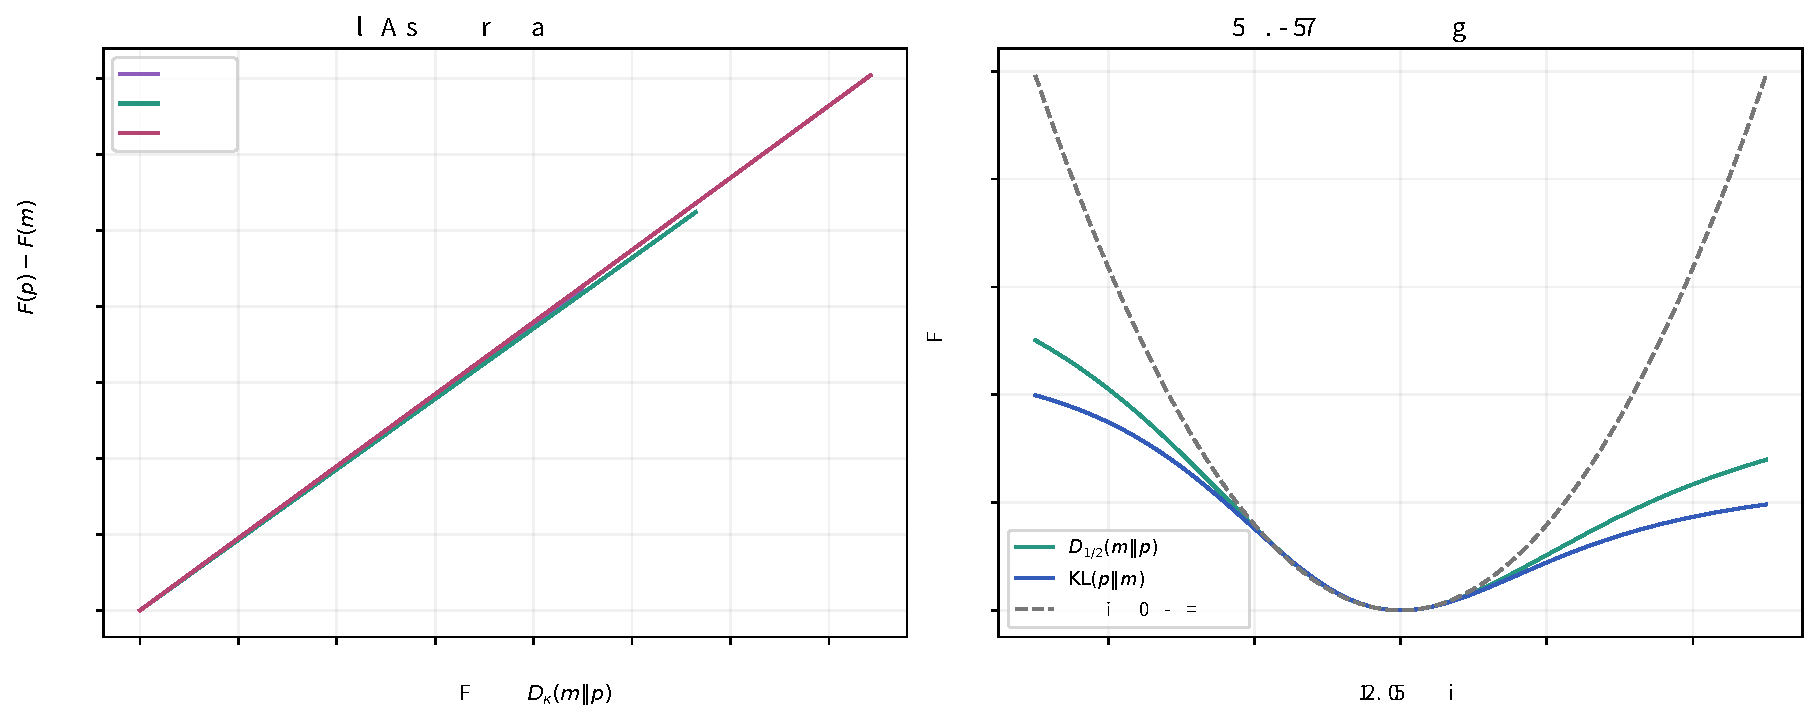
\includegraphics[width=\textwidth]{../../results/proximal-family-geometry/decomposition.pdf}
 \caption{左图检验 $F(p)-F(m)=Z^\kappa D_\kappa(m\Vert p)$，所有点位于对应常数斜率的直线上。右图固定同一个平方根 target，比较 Hellinger 与 reverse KL 拟合：共同的二阶曲率不消除远处损失的差异。}
\end{figure}

\subsection{精确外层与有限 inner 的散度进展}

\begin{theorem}[teacher 散度的进展恒等式]
\label{thm:proximal-teacher-progress}
记 $c_\kappa=Z^\kappa$，端点 $\kappa=0,1$ 取 $c_\kappa=1$。对任意候选 $p$，有
\begin{equation}
 \lambda\left[D_\kappa(t\Vert q)-D_\kappa(t\Vert p)\right]
 =(1-\lambda)D_\kappa(q\Vert p)
 +c_\kappa\left[D_\kappa(m\Vert q)-D_\kappa(m\Vert p)\right].
 \label{eq:proximal-progress-identity}
\end{equation}
若 $D_\kappa(m\Vert p)\le D_\kappa(m\Vert q)$，则 teacher 散度不会增加。精确更新 $p=m$ 且 $q\ne t$ 时严格下降。
\end{theorem}

\begin{proof}
$F(q)=\lambda D_\kappa(t\Vert q)$，而 $F(p)=(1-\lambda)D_\kappa(q\Vert p)+\lambda D_\kappa(t\Vert p)$。由定理~\ref{thm:proximal-barycenter-gap}，$F(q)-F(p)=c_\kappa[D_\kappa(m\Vert q)-D_\kappa(m\Vert p)]$。将 $F(q),F(p)$ 的定义代入并移项，即得恒等式。若目标散度改善，右侧两项非负；若 $p=m$、$q\ne t$，$m\ne q$，则至少第一项严格为正。最后，$m=q$ 会要求 $t_a^\kappa$ 与 $q_a^\kappa$ 成同一比例，概率归一化强制 $t=q$；两个端点同样成立。\hfill$\square$
\end{proof}

这给出了一个纯数学的 finite-inner 条件：降低本轮的 $D_\kappa(m\Vert p)$ 就能提高同一 $D_\kappa$ 下的 teacher 接近度。这里 teacher 散度的方向随 $\kappa$ 改变；一般 $\kappa$ 的保证不能直接替换成每步 $\KL(p\Vert t)$ 都下降。用其他拟合损失获得同一 target，只能在精确求解时自动继承本结论。

\subsection{连续极限是 teacher 散度的自然梯度流}

对 $\lambda\to0$，记 $\rho_a=t_a/q_a$、$A_\kappa=\E_q\rho^\kappa$。逐项展开 $h_a=q_a[1+\lambda(\rho_a^\kappa-1)/\kappa+O(\lambda^2)]$ 并归一化，得到
\begin{equation}
 m_a=q_a+\lambda v_{\kappa,a}+O(\lambda^2),\qquad
 v_{\kappa,a}=\frac{q_a}{\kappa}(\rho_a^\kappa-A_\kappa).
 \label{eq:proximal-natural-velocity}
\end{equation}
展开针对固定完整支持的 $q,t$；其余项不能在任意极端概率比上直接视为统一 $O(\lambda^2)$。$\kappa=0$ 的极限为 $v_{0,a}=q_a[\log\rho_a-\E_q\log\rho]$，$\kappa=1$ 为 $v_1=t-q$。

概率单纯形的 Fisher 度量为 $\langle v,w\rangle_q=\sum_av_aw_a/q_a$。若 $g_a=\partial L/\partial q_a$，则负自然梯度为 $-q_a(g_a-\E_qg)$：其分量和为零，且对任何切向量 $w$，Fisher 内积恰好等于 $-\sum_ag_aw_a$。取 $L(q)=D_\kappa(t\Vert q)$，有 $g_a=-\rho_a^\kappa/\kappa$，因此 $v_\kappa=-\operatorname{grad}_{\!F}D_\kappa(t\Vert q)$。连续时间 $\tau$ 下
\begin{equation}
 \frac{dq_a}{d\tau}=v_{\kappa,a},\qquad
 \frac{d}{d\tau}D_\kappa(t\Vert q)
 =-\|v_\kappa\|_F^2
 =-\frac1{\kappa^2}\Var_q(\rho^\kappa).
 \label{eq:proximal-flow-lyapunov}
\end{equation}
最后一步由 $\sum_av_a=0$ 及 $g^\top v=-(\E_q\rho^{2\kappa}-A_\kappa^2)/\kappa^2$ 得到。$\kappa=0$ 时右侧为 $-\Var_q(\log\rho)$。所有形状参数都对应同一 Fisher 度量，但所下降的全局 teacher 散度不同。

\subsection{escort 坐标中的线性轨迹与全局收敛}

对 $\kappa>0$ 定义 escort 分布和幂和
\begin{equation}
 E_\kappa(q)_a=\frac{q_a^\kappa}{S_\kappa(q)},\qquad
 S_\kappa(q)=\sum_aq_a^\kappa.
\end{equation}
$E_\kappa$ 是单纯形上的双射，逆映射为 $q_a\propto E_\kappa(q)_a^{1/\kappa}$。由 $m_a^\kappa=S_a/Z^\kappa$，共同的归一化因子在 escort 中消失，故
\begin{equation}
 E_\kappa(m)=(1-a)E_\kappa(q)+aE_\kappa(t),\qquad
 a=\frac{\lambda S_\kappa(t)}{(1-\lambda)S_\kappa(q)+\lambda S_\kappa(t)}.
 \label{eq:proximal-escort-step}
\end{equation}
这是精确式，不是局部近似。$\kappa=1$ 时 $S_1=1$，恢复 $a=\lambda$；$0<\kappa<1$ 时，$S_\kappa(q)=\exp((1-\kappa)H_\kappa(q))$，其中 $H_\kappa$ 是 Rényi 熵。因此固定的概率幂插值强度在 escort 坐标中表现为随分布熵改变的有效步幅。

\begin{figure}[htbp]
 \centering
 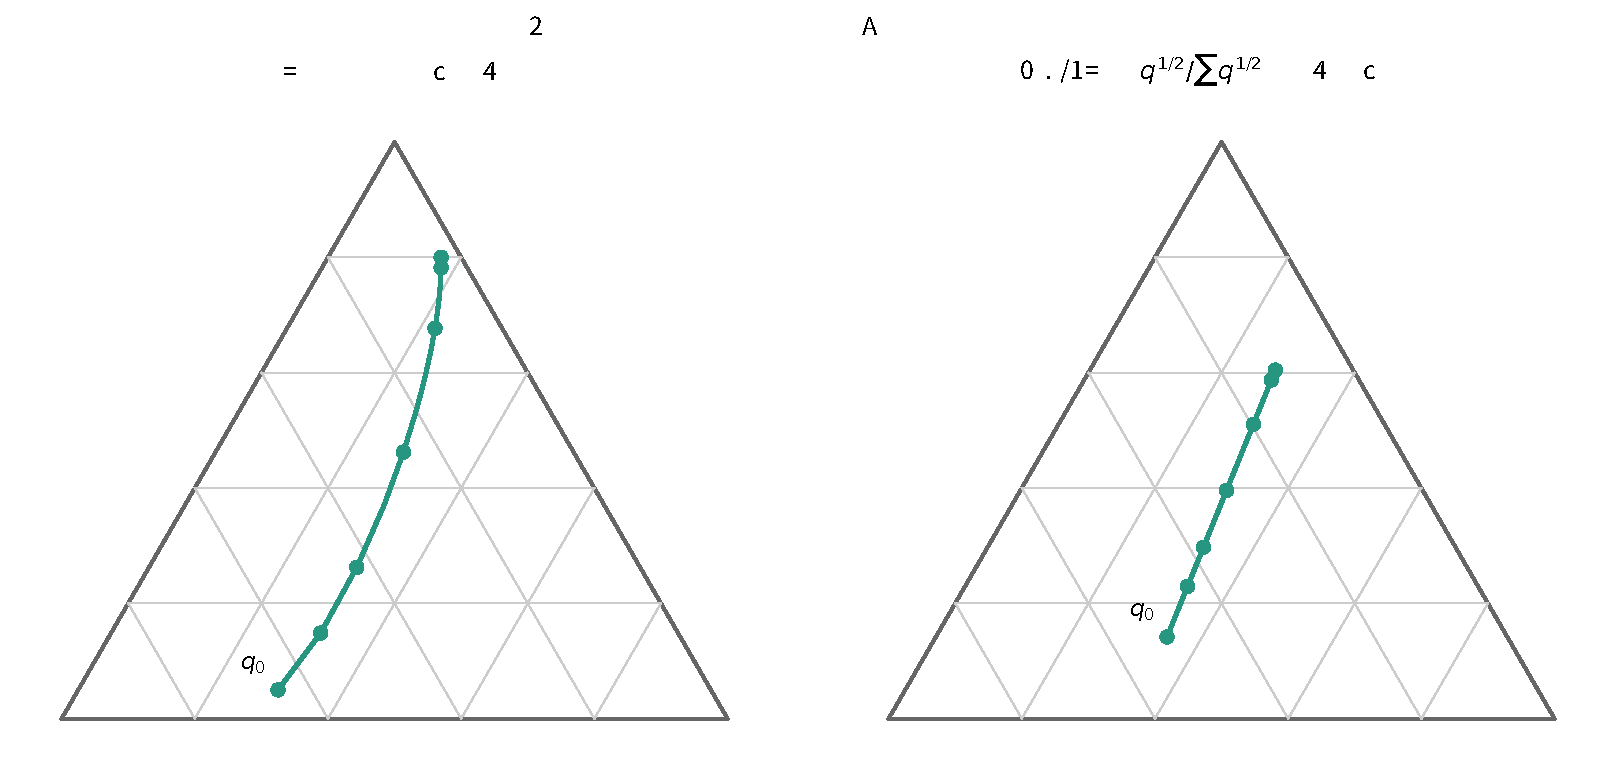
\includegraphics[width=\textwidth]{../../results/proximal-family-geometry/escort.pdf}
 \caption{同一平方根外层轨迹在概率坐标中弯曲，在 escort 坐标中是直线。圆点和数字表示迭代时点。高维分量在固定教师下共享一个进度系数。}
\end{figure}

若 $q_{k+1}=m_{\kappa,\lambda}(q_k,t)$，记 $e_k=E_\kappa(q_k)$，则
\begin{equation}
 e_k-e_t=b_k(e_0-e_t),\qquad
 b_k=\prod_{j=0}^{k-1}(1-a_j).
 \label{eq:proximal-escort-orbit}
\end{equation}
这将固定教师下的 $d-1$ 维精确外层轨迹归结为一个标量 $b_k$。对连续自然梯度流，$dq_a/d\tau=q_a(\rho_a^\kappa-A_\kappa)/\kappa$，所以
\begin{align}
 \frac{d}{d\tau}q_a^\kappa&=t_a^\kappa-A_\kappa q_a^\kappa,\\
 \frac{d}{d\tau}S_\kappa(q)&=S_\kappa(t)-A_\kappa S_\kappa(q),\\
 \frac{d}{d\tau}E_\kappa(q)&=\frac{S_\kappa(t)}{S_\kappa(q)}[E_\kappa(t)-E_\kappa(q)].
\end{align}
改用时间 $\sigma$，$d\sigma/d\tau=S_\kappa(t)/S_\kappa(q)>0$，就有 $e(\sigma)=e_t+e^{-\sigma}(e_0-e_t)$。离散步式~\eqref{eq:proximal-escort-step} 也位于同一条流轨迹上，对应时间增量 $-\log(1-a)$。精确幂均值步因此是这个自然梯度流轨迹的一种时间重参数化，而不只是具有相同起始切线。

\begin{theorem}[teacher 定向的 escort 收缩与误差累积]
\label{thm:proximal-escort-contraction}
令 $d$ 为词表大小，$0<\kappa\le1$，定义度量 $d_\kappa(q,t)=\|E_\kappa(q)-E_\kappa(t)\|_1$。对固定 teacher 的精确更新有
\begin{equation}
 d_\kappa(q_{k+1},t)=(1-a_k)d_\kappa(q_k,t)\le c\,d_\kappa(q_k,t),\quad
 c=\frac{(1-\lambda)d^{1-\kappa}}{(1-\lambda)d^{1-\kappa}+\lambda S_\kappa(t)}<1.
\end{equation}
故 $q_k\to t$。若近似更新满足 $d_\kappa(q_{k+1},m(q_k,t))\le\epsilon_k$，则
\begin{equation}
 d_\kappa(q_k,t)\le c^kd_\kappa(q_0,t)+\sum_{j=0}^{k-1}c^{k-1-j}\epsilon_j,
 \qquad
 \limsup_kd_\kappa(q_k,t)\le\frac{\epsilon_\infty}{1-c}
\end{equation}
其中最后一式要求 $\limsup_k\epsilon_k\le\epsilon_\infty$。
\end{theorem}

\begin{proof}
式~\eqref{eq:proximal-escort-step} 给出距离的精确比例。Jensen 不等式给出 $S_\kappa(q)\le d^{1-\kappa}$，因此 $1-a_k\le c$。反复应用得到精确更新的 $c^k$ 界；escort 逆映射连续，故 $q_k\to t$。近似更新时，三角不等式给出 $d_\kappa(q_{k+1},t)\le\epsilon_k+c\,d_\kappa(q_k,t)$，展开得到有限步式。对任意 $\delta>0$，取 $N$ 使 $j\ge N$ 时 $\epsilon_j\le\epsilon_\infty+\delta$。有限个早期项乘以 $c^{k-1-j}$ 后趋于零，后期项的和不超过 $(\epsilon_\infty+\delta)\sum_{i\ge0}c^i$。令 $\delta\to0$ 得极限上界。\hfill$\square$
\end{proof}

这是对固定 teacher 的定向收缩，不声称两个任意 anchor 经同一算子后具有同一个收缩系数；它也不直接等于原概率空间的 TV 收缩。$\kappa\to0$ 时，escort 本身趋于均匀分布，必须重标度才保留信息：
\begin{equation}
 \frac d\kappa\left[E_\kappa(q)_a-\frac1d\right]
 \longrightarrow\log q_a-\frac1d\sum_b\log q_b.
\end{equation}
几何端点就在这些中心化 log 坐标中满足精确比例 $1-\lambda$。在任何固定完整支持的 teacher 附近，所有 $\kappa$ 都有 $m(t+\delta,t)=t+(1-\lambda)\delta+O(\|\delta\|^2)$，因为 $a_k\to\lambda$。它们共享局部收敛率，远处的度量和有效时间则不同。

\begin{figure}[htbp]
 \centering
 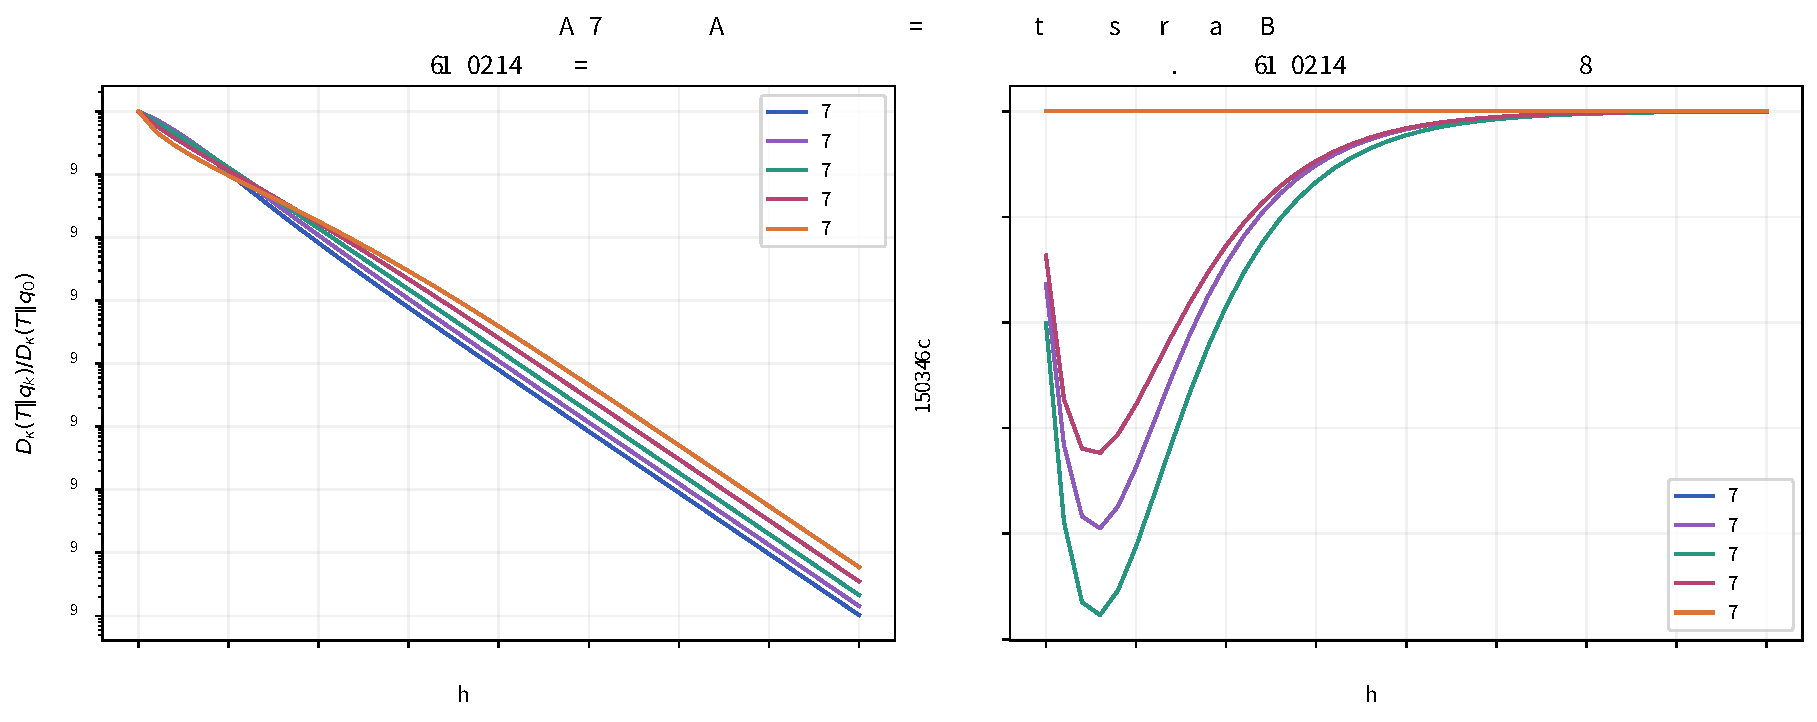
\includegraphics[width=\textwidth]{../../results/proximal-family-geometry/convergence.pdf}
 \caption{精确外层的 teacher 散度单调下降，有效 escort 步幅趋于共同的 $\lambda$。每条曲线使用各自的 $D_\kappa$ 并按初值归一化，图中的高低不能直接作为同一任务的训练性能排名。}
\end{figure}


\section{精确镜像下降的教师目标}
\label{sec:proximal-md-objective}

幂均值重心定义了 target，但尚未指定对固定教师最小化什么函数。本节从冻结信号积分出一个不依赖 anchor 的教师目标，证明有限步幂均值恰为其标准熵镜像下降（Mirror Descent，MD）。固定 $\kappa,\eta$ 和教师时目标不变；改变 $\eta$ 会同时改变目标与原更新步长。

\subsection{由冻结信号反求生成函数}

\begin{theorem}[幂均值信号的可积性与精确 MD 目标]
\label{thm:power-md-integrable-objective}
记 $A=A_{\kappa,\eta}$，定义规范化生成函数
\begin{equation}
 \omega_{\kappa,\eta}(x)
 =x\int_1^x\frac{A_{\kappa,\eta}(u)}{u^2}\,du,
 \qquad x>0,
 \label{eq:power-md-generator-integral}
\end{equation}
以及教师目标
\begin{equation}
 \mathcal J_{\kappa,\eta}(p;T)
 =D_{\omega_{\kappa,\eta}}(T\Vert p)
 =\sum_a p_a\omega_{\kappa,\eta}(T_a/p_a).
 \label{eq:power-md-fixed-objective}
\end{equation}
则 $\omega(1)=\omega'(1)=0$、$\omega''(x)>0$，$\mathcal J\ge0$ 且唯一零点为 $p=T$。在正正交象限内，$\mathcal J$ 的坐标梯度恰为
\begin{equation}
 \frac{\partial\mathcal J}{\partial p_a}(p;T)
 =-A_{\kappa,\eta}(T_a/p_a).
 \label{eq:power-md-exact-gradient}
\end{equation}
因此步长 $\eta$ 的 entropy MD 更新
\begin{equation}
 p^+=\argmin_{p\in\Delta}
 \left\{\langle\nabla\mathcal J(q;T),p-q\rangle
       +\frac1\eta\KL(p\Vert q)\right\}
 \label{eq:power-md-exact-step}
\end{equation}
严格等于幂均值 target $m_{\kappa,\eta}$。
\end{theorem}

\begin{proof}
对积分定义求导，得到
\begin{align}
 \omega'(x)&=\int_1^x\frac{A(u)}{u^2}\,du+\frac{A(x)}x,\\
 \omega(x)-x\omega'(x)&=-A(x),\\
 \omega''(x)&=\frac{A'(x)}x
 =\frac{x^{\kappa-2}}{1-\eta+\eta x^\kappa}>0.
 \label{eq:power-md-curvature}
\end{align}
最后一个式子对 $\kappa=0$ 按连续端点取值为 $1/x^2$。$A(1)=0$ 保证两项规范化条件。严格凸性给出 $\omega\ge0$，Jensen 等号条件和分布归一化给出散度的唯一零点。逐项使用链式法则，令 $x=T_a/p_a$，则
\begin{equation}
 \frac\partial{\partial p_a}[p_a\omega(T_a/p_a)]
 =\omega(x)-x\omega'(x)=-A(x).
\end{equation}
这一步把固定 anchor 上的信号提升为一个对任意当前分布 $p$ 定义的目标梯度。将它代入 MD 子问题，再对 $\sum p=1$ 引入乘子 $\nu$，有
\begin{equation}
 -A(T_a/q_a)+\eta^{-1}[\log(p_a/q_a)+1]+\nu=0.
\end{equation}
归一化后 $p_a^+\propto q_a\exp[\eta A(T_a/q_a)]$，正是前文的幂均值 target。该子问题严格凸，解唯一。

反过来，若规范化生成函数满足 $\omega-x\omega'=-A$，则 $(\omega/x)'=A/x^2$，连同 $\omega(1)=0$ 唯一确定式~\eqref{eq:power-md-generator-integral}。因此所构造的规范化函数是这一逐坐标梯度对应的唯一生成函数。
\end{proof}

\subsection{单调概率比信号的通用 $f$ 散度框架}

\begin{proposition}[单调信号的可积性与相对光滑性]
\label{prop:power-general-signal-framework}
设 $S:(0,\infty)\to\mathbb R$ 连续可微，$S(1)=0$、$S'(x)>0$。定义
\begin{equation}
 \omega_S(x)=x\int_1^x\frac{S(u)}{u^2}\,du,\qquad
 \mathcal J_S(p;T)=D_{\omega_S}(T\Vert p).
\end{equation}
则 $\omega_S$ 严格凸、规范化，且 $\nabla_p\mathcal J_S=-S(T/p)$。对该目标执行步长 $\tau$ 的熵 MD，精确解为 $p^+\propto q\exp[\tau S(T/q)]$。若
\begin{equation}
 L_S=\sup_{x>0}xS'(x)<\infty,
\end{equation}
则 $\mathcal J_S$ 相对于负熵 $H$ 为 $L_S$ 相对光滑；$0<\tau\le1/L_S$ 时具有本节单步下降与三点进展的相应保证。
\end{proposition}

\begin{proof}
积分微分给出 $\omega_S-x\omega_S'=-S$、$\omega_S''=S'/x>0$ 及 $\omega_S(1)=\omega_S'(1)=0$。透视函数求导后得到 $\nabla_p\mathcal J_S=-S(T/p)$，MD 一阶条件与归一化给出所列解。再令 $x_a=T_a/p_a$，有
\begin{equation}
 \nabla_p^2\mathcal J_S
 =\operatorname{diag}[x_aS'(x_a)/p_a]
 \preceq L_S\operatorname{diag}(1/p_a)=L_S\nabla^2H.
\end{equation}
沿连接两个正分布的线段积分 Hessian，得到相对光滑不等式。本节下降与三点证明只使用这个 Hessian 界、目标凸性和 MD 一阶条件，将 $1/\eta$ 替换成 $L_S$ 后逐步成立。
\end{proof}

幂均值信号属于这个框架，因为 $xA'(x)=x^\kappa/(1-\eta+\eta x^\kappa)\le1/\eta$。其他单调信号也可定义不同的凸教师目标；第~\ref{cor:power-general-signal-all-f}~推论进一步证明所列步幅下的共同教师散度进展。统一尾部界、可估计中心和良好的 BPO 投影仍需分别证明，可积性本身不保证这些额外性质。

\subsection{幂散度、reverse KL 与归一化 JS 的关系}

\begin{theorem}[精确 MD 目标的端点与曲率插值]
\label{thm:power-md-objective-endpoints}
固定正支持分布时，
\begin{align}
 \mathcal J_{0,\eta}(p;T)&=\KL(p\Vert T),\\
 \lim_{\eta\to0}\mathcal J_{\kappa,\eta}(p;T)&=D_\kappa(T\Vert p),\\
 \lim_{\eta\to1}\mathcal J_{\kappa,\eta}(p;T)&=\KL(p\Vert T).
 \label{eq:power-md-objective-limits}
\end{align}
算术形状 $\kappa=1$ 的有限 $\eta$ 目标为
\begin{equation}
 \boxed{\mathcal J_{1,\eta}(p;T)
 =\frac{(1-\eta)\KL(p\Vert M)+\eta\KL(T\Vert M)}{\eta(1-\eta)},
 \quad M=(1-\eta)p+\eta T.}
 \label{eq:power-md-js-endpoint}
\end{equation}
分子是权重为 $(1-\eta,\eta)$ 的 Jensen--Shannon（JS）散度。对所有 $x>0$，生成函数的曲率满足
\begin{equation}
 \frac1{\omega_{\kappa,\eta}''(x)}
 =\frac{1-\eta}{g_\kappa''(x)}+\frac\eta{g_0''(x)}.
 \label{eq:power-md-harmonic-curvature}
\end{equation}
所以精确 MD 目标以曲率的加权调和平均连接幂散度与 reverse KL；它一般不同于两种散度的加权和。
\end{theorem}

\begin{proof}
$\kappa=0$ 时 $A=\log x$，积分直接得到 $\omega=x-1-\log x=g_0$。在任意固定有限积分区间，$\eta\to0$ 时 $A\to(x^\kappa-1)/\kappa$，$\eta\to1$ 时 $A\to\log x$，而分母在该区间内有统一正下界。故可交换积分与极限。小 $\eta$ 时的极限生成函数与 $g_\kappa$ 有相同的二阶导数 $x^{\kappa-2}$ 及相同规范化条件；两者相等。有限词表允许逐项取散度极限。

对 $\kappa=1$，记 $a=1-\eta$、$B=a+\eta x$。分部积分给出
\begin{align}
 \omega_{1,\eta}(x)
 &=-\eta^{-1}\log B+x\int_1^x\frac{du}{u(a+\eta u)}\\
 &=\frac{x\log x}{a}-\left(\frac1\eta+\frac xa\right)\log B
 =\frac{\eta x\log x-B\log B}{\eta a}.
\end{align}
代入 $x=T/p$ 得到
\begin{equation}
 \mathcal J_{1,\eta}(p;T)
 =\frac{\eta\KL(T\Vert p)-\KL(M\Vert p)}{\eta a}.
\end{equation}
展开两项 KL，使用 $M=ap+\eta T$，其分子等于 $a\KL(p\Vert M)+\eta\KL(T\Vert M)$，得到式~\eqref{eq:power-md-js-endpoint}。最后，式~\eqref{eq:power-md-curvature} 的倒数为 $a x^{2-\kappa}+\eta x^2$；两项分别是 $a/g_\kappa''$ 与 $\eta/g_0''$。
\end{proof}

因此涉及两个 KL 方向的准确表述是：重心散度 $D_\kappa$ 在 $\kappa=0,1$ 分别为 reverse/forward KL；精确 MD 目标 $\mathcal J_{\kappa,\eta}$ 在固定正 $\eta$ 下的 $\kappa=1$ 端点是归一化加权 JS，随后令 $\eta\to0$ 才恢复 forward KL。中心 $K_{1,\eta}$ 则是 reverse KL 到混合分布，属于第三个对象。

对固定 $\kappa>0$，两个不同的插值强度一般也不能仅用目标的整体缩放互相替代。若 $\omega_{\kappa,\eta_1}=b\omega_{\kappa,\eta_2}$，则一处的二阶导数均为一，强制 $b=1$；式~\eqref{eq:power-md-curvature} 随后要求 $1-\eta_1+\eta_1x^\kappa=1-\eta_2+\eta_2x^\kappa$ 对所有 $x$ 成立，只能有 $\eta_1=\eta_2$。因此 $\eta$ 是教师目标的形状选择，同时也是原幂均值更新的 MD 步长；若要在同一个 $\mathcal J$ 上单独调节 MD 步长，应固定 $\eta$，另用后文的 $\tau$。

\begin{center}
\small
\begin{tabular}{lll}
\toprule
散度及用途 & $\kappa=0$ & $\kappa=1$、固定 $0<\eta<1$\\
\midrule
$D_\kappa(T\Vert p)$：定义重心 & $\KL(p\Vert T)$ & $\KL(T\Vert p)$\\
$\mathcal J_{\kappa,\eta}(p;T)$：精确 MD 目标 & $\KL(p\Vert T)$ & $\mathrm{JS}_\eta(p,T)/[\eta(1-\eta)]$\\
$K_{\kappa,\eta}(q,T)$：冻结教师中心 & $\KL(q\Vert T)$ & $\KL(q\Vert(1-\eta)q+\eta T)/\eta$\\
\bottomrule
\end{tabular}
\end{center}

\begin{theorem}[精确 MD 目标的锐统一上界]
\label{thm:power-md-uniform-cap}
若 $0<\kappa\le1$、$0<\eta<1$，定义
\begin{equation}
 c=-\frac{\log(1-\eta)}{\kappa\eta},\qquad
 d=\int_1^\infty\frac{A_{\kappa,\eta}(u)}{u^2}\,du.
\end{equation}
则 $0<d\le1/\eta$，并有
\begin{equation}
 0\le\mathcal J_{\kappa,\eta}(p;T)\le c+d.
 \label{eq:power-md-uniform-cap}
\end{equation}
上界不依赖词表维数，并且在至少二元的完整支持分布类上是锐上确界。算术形状满足
\begin{equation}
 c+d=\frac{-\eta\log\eta-(1-\eta)\log(1-\eta)}{\eta(1-\eta)}.
\end{equation}
原始 reverse KL 的 $\kappa=0$ 端点没有有限统一上界。
\end{theorem}

\begin{proof}
当 $u\ge1$，$A(u)>0$（除 $u=1$ 外），且 $1-\eta+\eta u^\kappa\le u^\kappa$，所以 $A(u)\le\log u/\eta$。又有 $\int_1^\infty(\log u)/u^2\,du=1$，得到 $0<d\le1/\eta$。积分定义给出 $\omega(x)/x\to d$（$x\to\infty$）。当 $x\to0$ 时 $A(x)\to-c$，写成
\begin{equation}
 \omega(x)=-x\int_x^1\frac{A(u)}{u^2}\,du\longrightarrow c.
\end{equation}
要核实最后一个极限，可对任意 $\epsilon>0$ 选取足够小的 $b$，使 $|A(u)+c|\le\epsilon$ 对 $u\le b$ 成立；区间 $[b,1]$ 的积分乘以 $x$ 趋零，区间 $[x,b]$ 的误差不超过 $\epsilon x(1/x-1/b)\le\epsilon$。

凸函数的导数不超过其无穷远渐近斜率 $d$，从零处积分可得 $\omega(x)\le c+dx$。对 $x=T/p$ 求 $p$ 期望，得到 $\mathcal J\le c+d$。取 $p=(\epsilon,1-\epsilon)$、$T=(1-\epsilon,\epsilon)$，则稀有 $p$ 坐标的贡献趋于 $d$，另一坐标的贡献趋于 $c$，证明锐性。算术形状的显式生成函数给出 $d=-\log\eta/(1-\eta)$，与 $c$ 相加得到归一化二元熵。$\kappa=0$ 时 $\omega=g_0$ 在零处发散，前述锐界退化为无穷大。
\end{proof}
\subsection{全局相对光滑、单步下降与外层收敛率}

\begin{theorem}[精确幂均值 MD 的下降与收敛]
\label{thm:power-md-relative-smoothness}
固定教师、$\kappa,\eta$，令 $H(p)=\sum_ap_a\log p_a$。在正单纯形内，$\mathcal J=\mathcal J_{\kappa,\eta}$ 相对于 $H$ 具有常数 $1/\eta$ 的相对光滑性：对任意正分布 $p,q$，
\begin{equation}
 \mathcal J(p;T)\le\mathcal J(q;T)+\langle\nabla\mathcal J(q;T),p-q\rangle
       +\eta^{-1}\KL(p\Vert q).
 \label{eq:power-md-relative-smoothness}
\end{equation}
若 $p^+\propto q\exp[\tau A(T/q)]$、$0<\tau\le\eta$，则
\begin{align}
 \mathcal J(q;T)-\mathcal J(p^+;T)
 &\ge\tau^{-1}\KL(q\Vert p^+)
  +(\tau^{-1}-\eta^{-1})\KL(p^+\Vert q),\\
 \tau\mathcal J(p^+;T)
 &\le\KL(T\Vert q)-\KL(T\Vert p^+).
 \label{eq:power-md-single-step-progress}
\end{align}
对每步刷新 anchor 的精确迭代 $q_{n+1}=p^+(q_n)$、步长 $0<\tau_n\le\eta$，有
\begin{equation}
 \mathcal J(q_N;T)\le
 \frac{\KL(T\Vert q_0)}{\sum_{n=0}^{N-1}\tau_n}.
 \label{eq:power-md-last-iterate-rate}
\end{equation}
特别地，$\tau_n=\eta$ 时每步就是幂均值 target，最后迭代误差不超过 $\KL(T\Vert q_0)/(\eta N)$。
\end{theorem}

\begin{proof}
记 $x_a=T_a/p_a$。根据式~\eqref{eq:power-md-exact-gradient}，目标在正正交象限的 Hessian 为
\begin{equation}
 \nabla_p^2\mathcal J(p;T)
 =\operatorname{diag}\left(\frac1{p_a}
       \frac{x_a^\kappa}{1-\eta+\eta x_a^\kappa}\right)
 \preceq\eta^{-1}\operatorname{diag}(1/p_a)
 =\eta^{-1}\nabla^2H(p).
 \label{eq:power-md-hessian-bound}
\end{equation}
对连接 $q,p$ 的线段积分二阶 Taylor 余项，得到相对光滑不等式。目标本身严格凸，其 Hessian 的每个对角元为正。

设 $g=\nabla\mathcal J(q;T)$。MD 的一阶条件给出 $g_a+\tau^{-1}\log(p_a^+/q_a)$ 为常数。与 $p^+-q$ 内积时常数消失，故
\begin{equation}
 \langle g,p^+-q\rangle
 =-\tau^{-1}[\KL(p^+\Vert q)+\KL(q\Vert p^+)].
\end{equation}
代入相对光滑式，得到第一个下降界。再用凸性 $\mathcal J(q;T)-\mathcal J(T;T)\le\langle g,q-T\rangle$，以及 $\mathcal J(T;T)=0$，得到
\begin{align}
 \mathcal J(p^+;T)
 &\le\langle g,p^+-T\rangle+\eta^{-1}\KL(p^+\Vert q)\\
 &=\tau^{-1}[\KL(T\Vert q)-\KL(T\Vert p^+)]
   -(\tau^{-1}-\eta^{-1})\KL(p^+\Vert q)\\
 &\le\tau^{-1}[\KL(T\Vert q)-\KL(T\Vert p^+)].
\end{align}
第二行使用熵 Bregman 的三点恒等式，可直接展开各 KL 核验。对 $n=0,\ldots,N-1$ 求和，非负的末项 KL 给出
\begin{equation}
 \sum_{n=0}^{N-1}\tau_n\mathcal J(q_{n+1};T)\le\KL(T\Vert q_0).
\end{equation}
由第一个下降界，$\mathcal J(q_N;T)\le\mathcal J(q_{n+1};T)$，故左侧至少为 $(\sum\tau_n)\mathcal J(q_N;T)$，得到最后迭代界。
\end{proof}

这个定理无需概率统一正下界，只要求给定有限分布严格为正；初始 $\KL(T\Vert q_0)$ 可以很大。若 $\sum\tau_n\to\infty$，则 $\mathcal J(q_N;T)\to0$，严格凸散度及有限单纯形紧性保证 $q_N\to T$。边界也不能形成额外的零点：由积分定义，
\begin{equation}
 \lim_{x\to\infty}\frac{\omega(x)}x
 =\int_1^\infty\frac{A(u)}{u^2}\,du=:d_\infty>0.
\end{equation}
该积分有限，因为 $0\le A(u)\le\log u/\eta$ 对 $u\ge1$ 成立。若某个坐标 $p_a\to0$，则 $p_a\omega(T_a/p_a)\to T_a d_\infty>0$。任何内点极限的零损失又强制各比率都等于一。因此所有收敛子列的极限只能是 $T$，整个序列收敛到 $T$。

对固定 anchor 的 BPO 内层，理想路径 $p_\xi\propto q\exp[\xi\eta A(T/q)]$、$0\le\xi\le1$ 对应从该 anchor 做一步步长为 $\tau=\xi\eta$ 的上述 MD；因而具有同一单步界。这里的外层收敛率要求每步重新计算信号并刷新 anchor。实际共享参数 BPO/AdamW 只有近似投影时，需要另外控制拟合误差；任意 BPO loss 下降不能自动套用该定理。若外层改变 $\eta$ 或 $\kappa$，目标 $\mathcal J$ 也改变，不能把各步的不等式直接望远镜求和。

\subsection{保留 KL 子问题与保留原教师目标的 MD 有别}

标准 entropy MD 对一个固定目标 $F$ 执行
\begin{equation}
 p^+=\argmin_p\{\langle\nabla F(q),p-q\rangle+\eta^{-1}\KL(p\Vert q)\}.
\end{equation}
取 $F_0(p)=\KL(p\Vert T)$，有 $\nabla F_0(q)=\log(q/T)+1$，与 $-r$ 只差常数，因而 $\kappa=0$ 的几何目标就是对原 reverse KL 的标准 entropy MD。

若 $\kappa>0$，有效梯度为 $-A_{\kappa,\eta}$，它本身依赖 $\eta$。其导数对 $r$ 为
\begin{equation}
 \frac{d}{dr}A_{\kappa,\eta}(e^r)=\frac{e^{\kappa r}}{1-\eta+\eta e^{\kappa r}}.
\end{equation}
当 $0<\eta<1$ 时它不是恒等于一的常数，所以一般不能用一个标量重新设定步长恢复原来的 $-r$ 方向。式~\eqref{eq:power-bpo-mirror-subproblem} 是精确的 entropy mirror 子问题，但不能称为对原 $F_0$ 的同一个 MD 更新。$\eta=1$ 或 $q=T$ 是特殊退化情况。信号依赖 $\eta$ 不妨碍为每个固定 $(\kappa,\eta)$ 构造另一个不依赖 anchor 的目标；本节已经给出新目标 $\mathcal J$ 的生成函数及收敛证明。

\subsection{连续极限是 teacher 散度的自然梯度流}

对 $\eta\to0$，记 $\rho_a=T_a/q_a$、$a_\kappa=\E_q\rho^\kappa$。逐项展开 $h_a=q_a[1+\eta(\rho_a^\kappa-1)/\kappa+O(\eta^2)]$ 并归一化，得到
\begin{equation}
 m_a=q_a+\eta v_{\kappa,a}+O(\eta^2),\qquad
 v_{\kappa,a}=\frac{q_a}{\kappa}(\rho_a^\kappa-a_\kappa).
 \label{eq:proximal-natural-velocity}
\end{equation}
展开针对固定完整支持的 $q,T$；其余项不能在任意极端概率比上直接视为统一 $O(\eta^2)$。$\kappa=0$ 的极限为 $v_{0,a}=q_a[\log\rho_a-\E_q\log\rho]$，$\kappa=1$ 为 $v_1=T-q$。

概率单纯形的 Fisher 度量为 $\langle v,w\rangle_q=\sum_av_aw_a/q_a$。若 $g_a$ 是 $L$ 的概率梯度代表，则负自然梯度为 $-q_a(g_a-\E_qg)$：其分量和为零，且对任何切向量 $w$，Fisher 内积恰好等于 $-\sum_ag_aw_a$。取 $L(q)=D_\kappa(T\Vert q)$，可取 $g_a=-\rho_a^\kappa/\kappa$；规范化生成函数给出的代表为 $(1-\rho_a^\kappa)/\kappa$，相差的常数被中心化消掉。因此 $v_\kappa=-\operatorname{grad}_{\!F}D_\kappa(T\Vert q)$。连续时间 $t$ 下
\begin{equation}
 \frac{dq_a}{dt}=v_{\kappa,a},\qquad
 \frac{d}{dt}D_\kappa(T\Vert q)
 =-\|v_\kappa\|_F^2
 =-\frac1{\kappa^2}\Var_q(\rho^\kappa).
 \label{eq:proximal-flow-lyapunov}
\end{equation}
最后一步由 $\sum_av_a=0$ 及 $g^\top v=-(\E_q\rho^{2\kappa}-a_\kappa^2)/\kappa^2$ 得到。$\kappa=0$ 时右侧为 $-\Var_q(\log\rho)$。所有形状参数都对应同一 Fisher 度量，但所下降的全局 teacher 散度不同。
\subsection{对固定幂散度执行有限步 MD 的另一种更新}

若要求在有限步长下严格采用这个固定 $F_\kappa$ 的 entropy MD，应另取
\begin{equation}
 \widetilde m_a\propto q_a
   \exp\left(\tau\frac{(T_a/q_a)^\kappa-1}{\kappa}\right).
 \label{eq:power-bpo-true-md-variant}
\end{equation}
它与幂均值目标只有一阶一致，有限 $\tau$ 时一般不同；并且指数中的概率比幂会重新引入极端正信号。另一种解释是第~\ref{sec:power-projection}~节 escort 坐标中的自适应二次目标梯度步，但这改变了坐标和目标，不应据此给实际神经网络 inner 更新贴上标准 MD 标签。

直接把 $D_\kappa(q\Vert p)$ 当成原负熵的 Bregman 正则也不正确：对 $0<\kappa<1$，它对 $p$ 的 Hessian 为 $\operatorname{diag}(q_a^\kappa p_a^{-\kappa-1})$，依赖参照 $q$。固定 mirror 势的 $B_\Phi(p,q)$ 对第一自变量的 Hessian 是 $\nabla^2\Phi(p)$，不依赖 $q$。一般情况下，两者不是同一 Bregman 散度。


\section{单 rollout 的 BPO 算法与内层拟合}
\label{sec:power-bpo-algorithm}

本节在第~\ref{sec:power-setup}~节定义的单教师、单 rollout 和冻结前缀测度上拟合 target。外层锚点 $q_n$ 与教师信号冻结，内层学生 $p_{n,j}$ 及其条件中心随参数更新。所有微分均不穿过 rollout、前缀权重、锚点与教师。

\subsection{形状参数只进入冻结监督信号}

使用式~\eqref{eq:proximal-power-signal} 与式~\eqref{eq:center-explicit-definition} 的冻结 $f,A$。目标构造已经由前两节证明，下面将它接到 BPO 的条件回归目标。

从下面的 KL mirror 子问题开始：
\begin{equation}
 m=\argmax_{p\in\Delta}
 \left\{\sum_a p_a A_{\kappa,\eta}(a)
       -\frac1\eta\KL(p\Vert q)\right\}.
 \label{eq:power-bpo-mirror-subproblem}
\end{equation}
根据第~\ref{thm:power-md-integrable-objective}~定理，其唯一解为
\begin{equation}
 m_a=q_ae^{f_a}/Z,\qquad Z=\sum_bq_be^{f_b}.
 \label{eq:power-bpo-explicit-target}
\end{equation}
改变 $\kappa$ 改变冻结监督和 target；KL 正则仍为 $\KL(p\Vert q)$。BPO 内层拟合这个 target，通常不直接最小化重心目标 $F$ 或教师目标 $\mathcal J$。

\subsection{BPO 损失、中心和精确梯度}

令 $C_qh=h-\E_qh$，定义
\begin{align}
 b_\theta&=\E_q[U_\theta-f],\\
 R_\theta(a)&=U_\theta(a)-f_a-b_\theta
            =C_q\log(p_\theta/m)_a,\\
 \mathcal L_n(\theta)
 &=\E_{s\sim\widehat d_n}\frac1{2\eta}
     \E_{a\sim q_n(\cdot\mid s)}R_\theta(s,a)^2.
 \label{eq:power-bpo-population-loss}
\end{align}
等价地，令 $\delta=C_q[U_\theta/\eta-A]$，则 $\mathcal L_n=(\eta/2)\E_{\widehat d_n,q}\delta^2$。$\kappa=0$ 时正好恢复原 BPO 的归一化损失。$\log Z$ 被 $C_q$ 消掉，因此无需显式计算 target 的归一化常数。teacher 监督只需本轮缓存 $f$ 及 $\E_qf$；学生项 $\E_qU_\theta$ 必须随 inner 参数更新，不能连同 teacher 中心一起冻结。

对固定 prefix，$\psi_\theta(a)=\nabla_\theta\log p_\theta(a)$。由于 $\nabla b_\theta=\E_q\psi_\theta$ 与 $\E_qR_\theta=0$，直接微分得到
\begin{align}
 \nabla_\theta\mathcal L_s
 &=\frac1\eta\E_q[R_\theta(\psi_\theta-\E_q\psi_\theta)]\\
 &=\frac1\eta\E_q[R_\theta\psi_\theta].
 \label{eq:power-bpo-gradient}
\end{align}
所以精确 BPO 不带 $p/q$ 重要性比率；测度就是冻结 $q$。若使用随机 action 估计最后一个期望，系数 $\sg(R_\theta/\eta)$ 乘以 $\log p_\theta(a)$ 给出所需 score 梯度。若直接微分完整平方损失，中心可以正常参与自动微分，其导数因精确零均值而抵消；两种停止梯度语义不能混为一谈。

用已定义的冻结中心 $K$ 展开 BPO 系数，得到
\begin{equation}
 \frac{R(a)}\eta
 =\frac{U(a)+\KL(q\Vert p)}\eta-A_{\kappa,\eta}(a)-K_{\kappa,\eta}.
\end{equation}
因此需要同时替换 action 监督 $r\mapsto A$ 和冻结教师中心 $\KL(q\Vert T)\mapsto K_{\kappa,\eta}$；只改变 action 监督却沿用原教师中心会产生偏差。$\kappa=0$ 时 $K_{0,\eta}=\KL(q\Vert T)$，恢复原接口。一般 $\kappa$ 下，由 $\E_qf=-\KL(q\Vert m)+\log Z$，有 $K_{\kappa,\eta}=[\KL(q\Vert m)-\log Z]/\eta$，它不是原 teacher KL。学生中心仍是当轮不断重算的 $\KL(q\Vert p)$。

完整支持下 $\mathcal L_s=0$ 当且仅当 $\log(p_a/m_a)$ 对全部 action 是常数。归一化强制该常数为零，因此 $p=m$。多 prefix、共享参数时，零损失还要求网络能同时表示全部条件 target；不可实现时只是 BPO 投影，不能宣称等于理想 mirror 更新。
\subsection{完整词表求和与一条轨迹的 action 估计}

一条 rollout 足以给出训练前缀，并不要求损失只使用每个前缀实际生成的一个 token。若能访问该前缀完整 $q,T,p$ 概率，可以直接求式~\eqref{eq:power-bpo-population-loss} 的 action 期望，仍然只有一次 response 生成，没有辅助 rollout 或候选组。这是本节的精确参考算法。

若只使用 rollout 中的 action，估计量为 $g(a)=R_\theta(a)\psi_\theta(a)/\eta$。对固定的 $s,\theta$ 和独立 $a\sim q(\cdot\mid s)$，它无偏。只用这一 action 同时估计本前缀的中心会令 $R=0$，使算法退化；把一条 response 的不同前缀 token 当作同一条件分布的组均值，也不能得到 $\E_{q(\cdot\mid s)}$。

复用整条已采样轨迹做 $I>1$ 个 inner 更新时，当前 $\theta$ 依赖已见 action，因而不再自动具有上述条件无偏性。给定固定样本 $a$，其平方残差损失的真正梯度是
\begin{equation}
 \nabla_\theta\frac{R_\theta(a)^2}{2\eta}
 =\frac{R_\theta(a)}\eta(\psi_\theta(a)-\E_q\psi_\theta),
\end{equation}
一般不等于停止系数的 $R_\theta(a)\psi_\theta(a)/\eta$。后者仍可作为 BPO population-gradient 的采样近似，但必须记录样本复用误差。对完整 rollout 的无偏性论证，还需 action 权重在抽取该 action 之前可确定；使用随机最终长度作分母是比率估计，不能直接套用逐条件无偏公式。完整词表求和对已冻结的经验前缀测度给出精确梯度，不受这些 action 估计问题影响。
\subsection{BPO 是带冻结测度的拟合损失}

对冻结 $q,m$，BPO population 损失是
\begin{equation}
 \mathcal L_{\mathrm{BPO}}(p;m,q)
 =\frac1{2\eta}\Var_q\!\left[\log\frac p m\right].
 \label{eq:divergence-map-bpo-loss}
\end{equation}
它一般不能写成仅以 $(p,m)$ 为自变量的 $D_g(p\Vert m)$。取二元词表，固定 $p,m$ 且 $\ell_1=\log(p_1/m_1)\ne\ell_2=\log(p_2/m_2)$，则
\begin{equation}
 \mathcal L_{\mathrm{BPO}}=\frac{q_1(1-q_1)}{2\eta}(\ell_1-\ell_2)^2.
\end{equation}
改变第三个分布 $q$ 会改变损失，任何固定生成函数的 $D_g(p\Vert m)$ 都不随 $q$ 改变。完整支持下，BPO 与 target 散度共享唯一零点 $p=m$，这一事实不意味着损失、曲率或有限步轨迹相同。

取切向扰动 $p=m+v$、$\sum_av_a=0$，并令全部 $v_a/m_a$ 一致趋零。展开 $\log(1+v_a/m_a)$ 得到
\begin{equation}
 \mathcal L_{\mathrm{BPO}}(m+v;m,q)
 =\frac1{2\eta}\left\{\sum_aq_a\frac{v_a^2}{m_a^2}
 -\left(\sum_aq_a\frac{v_a}{m_a}\right)^2\right\}
 +O\!\left(\max_a|v_a/m_a|^3\right).
\end{equation}
若 $q=m$，一次均值为 $\sum v=0$，二阶项恢复 $\sum v_a^2/m_a$ 的 Fisher 度量，另带 $1/\eta$。一般冻结 $q\ne m$ 时，BPO 的局部度量与 target 上的 Fisher 度量不同。若使用独立 logits $z$，则 $C_q\log(p/m)=C_q(z-\log m)$，全局 Hessian 为 $[\operatorname{diag}(q)-qq^\top]/\eta$，与 $\kappa$ 无关。

\subsection{BPO 的固定几何与有限 inner 性质}

令独立 logits 为 $z$，$p=\operatorname{softmax}(z)$。由于 $C_q$ 消掉 softmax 的归一化常数，单 prefix 损失成为
\begin{align}
 \mathcal L_s(z)&=\frac1{2\eta}
    (z-\log m)^\top Q_q(z-\log m),\\
 Q_q&=\operatorname{diag}(q)-qq^\top,\qquad
 \nabla_z\mathcal L_s=Q_q(z-\log m)/\eta,\\
 \nabla_z^2\mathcal L_s&=Q_q/\eta.
\end{align}
$Q_q$ 在常数方向为零，在 $\boldsymbol1^\perp$ 上正定。对 $v\perp\boldsymbol1$，
\begin{equation}
 v^\top Q_qv=\sum_aq_a(v_a-\E_qv)^2
 \ge q_{\min}\sum_a(v_a-\E_qv)^2
 \ge q_{\min}\|v\|^2.
\end{equation}
Gershgorin 界给出 $\lambda_{\max}(Q_q)\le\max_a2q_a(1-q_a)\le1/2$。独立 logits 的普通梯度下降因此在 $0<\alpha_{\mathrm{opt}}<2\eta/\lambda_{\max}(Q_q)$ 下收敛；$\alpha_{\mathrm{opt}}<4\eta$ 是充分条件。若 $h=z-\log m$ 的第 $i$ 个非零特征方向系数为 $c_i$，则
\begin{equation}
 \mathcal L_s(z_j)=\frac1{2\eta}\sum_i\lambda_i c_i^2
    (1-\alpha_{\mathrm{opt}}\lambda_i/\eta)^{2j}.
\end{equation}
这些是独立 logits 的精确结论，不是 AdamW 或共享神经网络的无条件收敛定理。固定 $q,\eta$ 时 $\kappa$ 完全不出现在 Hessian 中：它改变回归目标与起始残差，不改善这个二次问题的条件数。小 $\eta$ 会增大曲率，并不自动降低归一化后的起始梯度。

若 $\|\psi_\theta(a)\|\le S$，随机 action 梯度有
\begin{equation}
 \E_q\|g\|^2\le\frac{2S^2}{\eta}\mathcal L_s.
\end{equation}
在 $p=q$ 时 $R=-C_qf$，故 $\mathcal L_s(q)=\Var_q(f)/(2\eta)$。在可实现的 $p=m$ 处，每个 action 的残差和随机梯度都为零。因而 target 形状影响初始监督尾部，而 BPO 拟合本身提供残差下降时的噪声控制；两者承担不同作用。

BPO 损失下降并不自动意味着 teacher KL 或 $D_\kappa$ 下降。一个三元反例取 $q=(0.4999995,0.4999995,10^{-6})$、$T=(0.8,0.199999,10^{-6})$、$\eta=0.3$、$\kappa=0.5$。令 $p\propto m\exp(0,0,12)$。稀有 action 的 logit 误差由很小的 $q$ 权重计价，BPO 损失低于起点，却会显著提高 $\KL(p\Vert T)$。本节核验程序给出 $\mathcal L_s(q)=0.06227708$、$\mathcal L_s(p)=0.00024000$，而 $\KL(q\Vert T)=0.22314483$、$\KL(p\Vert T)=1.65421904$。因此有限 inner 仍需真 teacher 散度和拟合误差证书。

若在该 prefix 上控制 $\|R\|_\infty\le\epsilon$，记 $\ell=\log(p/m)=R+c$。由概率归一化 $c=-\log\E_me^R\in[-\epsilon,\epsilon]$，得到 $\|\ell\|_\infty\le2\epsilon$ 和 $\KL(p\Vert m)\le2\epsilon$。仅从 BPO 损失可保证 $\|R\|_\infty\le\sqrt{2\eta\mathcal L_s/q_{\min}}$，可以取这个上界为 $\epsilon$；大词表极小的 $q_{\min}$ 会使该保证很弱。这解释了精确最优点一致与有限拟合质量之间的差距。
\subsection{锚点 Fisher 预条件的 BPO 保留有限步镜像性质}

前面的反例允许任意候选 $p$。如果约束 inner 的实际路径，可以得到比零误差最优点更强的保证。仍使用独立 logits，令 $Q_q^+$ 为 $Q_q$ 的 Moore--Penrose 逆，采用冻结锚点 Fisher 预条件更新
\begin{align}
 z^+&=z-\gamma\eta Q_q^+\nabla_z\mathcal L_s
     =z-\gamma Q_q^+Q_q(z-\log m),\\
 p^+_a&\propto p_a^{1-\gamma}m_a^\gamma,\qquad 0<\gamma\le1.
 \label{eq:power-bpo-anchor-fisher-step}
\end{align}
由于 $Q_q^+Q_q$ 是 $\boldsymbol1^\perp$ 上的正交投影，它与恒等映射只差常数 logit；softmax 消掉该常数。因此上式是精确的分布恒等式。$Q_q$ 是锚点 $q$ 的 Fisher，不能改称当前 $p$ 的 Fisher。该更新也恰好等于以当前 $p$ 为 KL 正则参照、步幅 $\gamma$ 对固定拟合目标 $\KL(p\Vert m)$ 执行 entropy MD。这里的 KL 目标是本轮 $m$，不等于原教师目标 $T$。

从 $p_0=q$ 出发，允许每次 $0<\gamma_j\le1$，归纳得到
\begin{align}
 p_j&=p_{\xi_j},\qquad
 p_{\xi,a}=q_ae^{\xi f_a}/Z_\xi,\\
 \xi_j&=1-\prod_{h<j}(1-\gamma_h),\qquad
 \mathcal L_s(p_j)=(1-\xi_j)^2\mathcal L_s(q).
 \label{eq:power-bpo-finite-inner-path}
\end{align}
证明只需代入 $\log(p_\xi/q)=\xi f-\log Z_\xi$，于是 $R_\xi=-(1-\xi)C_qf$；再对几何插值的 log 密度求线性组合，得到 $\xi^+=\xi+\gamma(1-\xi)$。这个理想 inner 的损失收缩因子不依赖 $q_{\min}$ 或词表大小，因为预条件器消掉了 $Q_q$ 的非零谱；实际计算与神经网络可实现性另有成本。

\begin{theorem}[幂均值 BPO 镜像拟合路径的有限步 teacher 进展]
\label{thm:power-bpo-inner-all-f}
在完整正支持、$\kappa\in[0,1]$、$0<\eta\le1$ 下，对任意凸函数 $\Phi$、$\Phi(1)=0$，令
\begin{equation}
 D_\Phi(p\Vert T)=\sum_aT_a\Phi(p_a/T_a).
\end{equation}
沿 $p_\xi\propto qe^{\xi f}$、$0\le\xi\le1$，$D_\Phi(p_\xi\Vert T)$ 不增加。因而式~\eqref{eq:power-bpo-anchor-fisher-step} 从 $q$ 出发时，每个有限 inner 都不增加 teacher 双向 KL、总变差或平方 Hellinger 距离。
\end{theorem}

\begin{proof}
记 $r_a=\log(T_a/q_a)$。$f(r)$ 单调递增；当 $\kappa>0$ 时 $f'(r)=\eta e^{\kappa r}/(1-\eta+\eta e^{\kappa r})\le1$，$\kappa=0$ 时 $f'=\eta\le1$。于是
\begin{equation}
 u_{\xi,a}=\frac{p_{\xi,a}}{T_a}
 =\frac{\exp[-r_a+\xi f(r_a)]}{Z_\xi}
\end{equation}
作为 $r_a$ 的函数单调不增，因为 $-1+\xi f'(r)\le0$。对于可微凸 $\Phi$，$\Phi'(u)$ 随 $u$ 单调不减，所以 $\Phi'(u_\xi(r))$ 随 $r$ 单调不增。微分归一化密度给出 $\partial_\xi p_\xi=p_\xi(f-\E_{p_\xi}f)$，因此
\begin{align}
 \frac{d}{d\xi}D_\Phi(p_\xi\Vert T)
 &=\operatorname{Cov}_{p_\xi}(\Phi'(u_\xi),f)\\
 &=\frac12\sum_{a,b}p_{\xi,a}p_{\xi,b}
   [\Phi'(u_{\xi,a})-\Phi'(u_{\xi,b})](f_a-f_b)
 \le0.
\end{align}
每个乘积非正，因为两因子对 $r$ 的单调性相反。有限词表和完整正支持下，$\{u_{\xi,a}:\xi\in[0,1],a\in\mathcal V\}$ 位于一个紧的正区间。任意有限凸函数都可在该区间由光滑凸函数一致逼近，逐点极限保留上述非增加关系，得到不可微情形。取 $\Phi(u)=u\log u$、$-\log u$、$|u-1|/2$ 与 $(\sqrt u-1)^2$，分别给出双向 KL、总变差与平方 Hellinger。\hfill$\square$
\end{proof}

对固定前缀测度逐条件求加权和保留该保证。任意降低 BPO 损失的候选则没有这项性质。共享神经网络、随机梯度、Fisher 近似和前缀测度刷新都可能离开指定路径，需要分别控制误差。

\begin{corollary}[通用单调信号 MD 的共同教师散度进展]
\label{cor:power-general-signal-all-f}
采用第~\ref{prop:power-general-signal-framework}~命题的 $S$，设 $L_S<\infty$、$0<\tau\le1/L_S$。则沿
\begin{equation}
 p_\xi\propto q\exp[\xi\tau S(T/q)],\qquad0\le\xi\le1,
\end{equation}
任意凸 $f$ 散度 $D_\Phi(p_\xi\Vert T)$ 都非增加。因此该步幅条件既保证对应教师目标 $\mathcal J_S$ 的 MD 下降，也保证其他凸生成教师散度不增加。
\end{corollary}

\begin{proof}
记 $r=\log(T/q)$、$f(r)=\tau S(e^r)$。则 $f'(r)=\tau e^rS'(e^r)\in(0,1]$。前一定理的证明仅使用 $f$ 单调递增和 $f'\le1$，未在协方差非正的论证中使用幂均值的其他性质，故逐步适用于此处的 $f$。
\end{proof}

\begin{figure}[htbp]
 \centering
 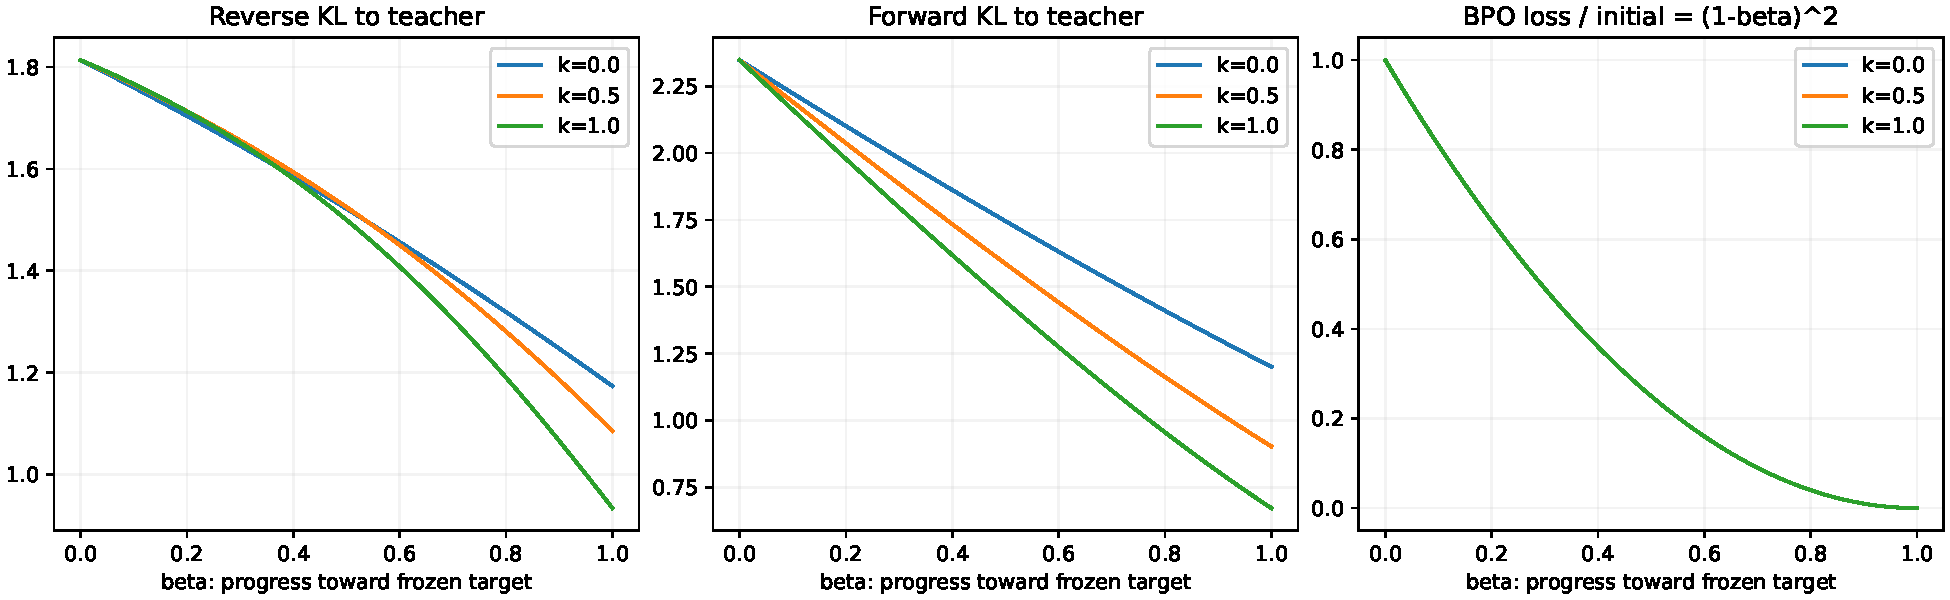
\includegraphics[width=\textwidth]{../../results/power-bpo-algorithm/finite-inner-progress.pdf}
 \caption{理想锚点 Fisher 预条件 BPO 的有限 inner：双向 teacher KL 沿 $\xi$ 下降，BPO 损失按 $(1-\xi)^2$ 精确收缩。图中旧记号 $\beta$ 对应本章 $\xi$；曲线为三元完整支持分布的解析求和。}
\end{figure}
\subsection{精确参考算法与实际 outer 更新}

\begin{algorithm}[htbp]
\caption{单 rollout 的幂均值 BPO\\{\small\textit{Semantics: 根据正文重构；完整词表条件期望}}}
\begin{algorithmic}[1]
\Require 教师 $T$，初始参数 $\theta_0$，prompt 测度 $\mathcal D$，batch 大小 $B\ge1$
\Require $0<\eta\le1$，$0\le\kappa\le1$，outer 预算 $N\ge1$，inner 次数 $I\ge1$
\For{outer $n=0,\ldots,N-1$}
    \State $q_n\gets\sg(\pi_{\theta_n})$
    \State $x_1,\ldots,x_B\overset{\mathrm{iid}}\sim\mathcal D$
    \For{每个 prompt 槽位 $x_i$}
        \State $y_i\sim q_n(\cdot\mid x_i)$ \Comment{恰好一条 rollout}
        \State 冻结其有效前缀与权重；若无有效前缀，跳过该槽位
        \For{每个有效前缀 $s$}
            \State 缓存 $q_n(\cdot\mid s)$，$f_s\gets\sg(f_{\kappa,\eta}(\log(T/q_n)))$，$\bar f_s\gets\E_{q_n}f_s$
        \EndFor
    \EndFor
    \If{所有槽位均无有效前缀}
        \State $\theta_{n+1}\gets\theta_n$
        \State 跳过本轮更新，重新采样下一批 prompt
    \Else
        \State $\theta_{n,0}\gets\theta_n$
        \For{$j=0,\ldots,I-1$}
            \State $U_{s,a}\gets\log(\pi_{\theta_{n,j}}(a\mid s)/q_n(a\mid s))$
            \State $R_{s,a}\gets U_{s,a}-f_{s,a}-\E_{q_n}(U_s-f_s)$
            \State $\mathcal L\gets\sum_sw_s\sum_aq_n(a\mid s)R_{s,a}^2/(2\eta)$
            \State $\theta_{n,j+1}\gets\theta_{n,j}-\alpha_{\mathrm{opt}}\nabla_\theta\mathcal L$
        \EndFor
        \State $\theta_{n+1}\gets\theta_{n,I}$ \Comment{本轮结束后才更新锚点并生成新 rollout}
    \EndIf
\EndFor
\State \Return $\theta_N$
\end{algorithmic}
\end{algorithm}

算法的有限预算、EOS 和最大生成长度由实验 setting 给定。每次 inner 都重新计算学生中心；教师信号与行为测度在整个 inner 窗口保持冻结。实验采用 AdamW 时只替换参数优化器，理想 target 与 BPO 损失不变，但上面的 logits 收敛式不随之自动成立。固定响应池的单 outer 扫描只检验 inner 拟合，不等于已经运行这个多 outer 算法。

\begin{figure}[htbp]
 \centering
 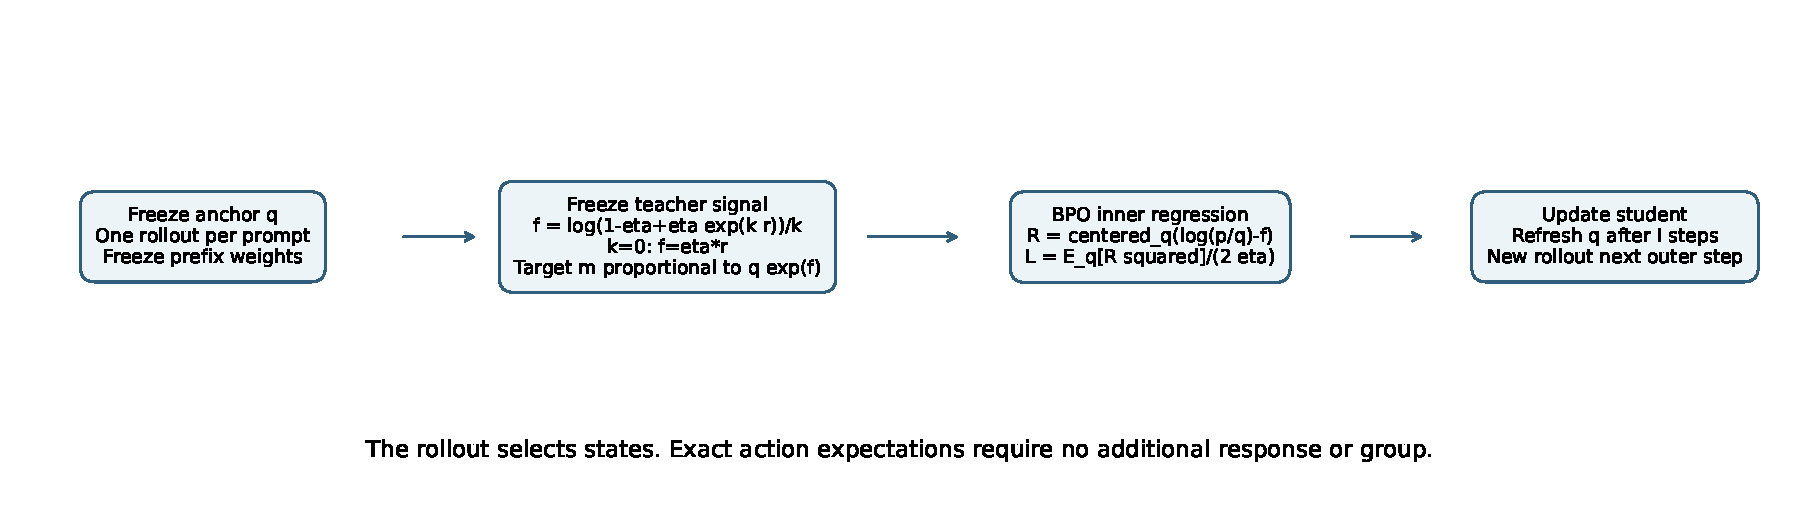
\includegraphics[width=\textwidth]{../../results/power-bpo-algorithm/pipeline.pdf}
 \caption{一条 response 选择前缀，幂均值形状决定冻结监督，BPO 以冻结 $q$ 的条件方差拟合。完整词表求和不需要增加 response 数量。}
\end{figure}
\begin{figure}[htbp]
 \centering
 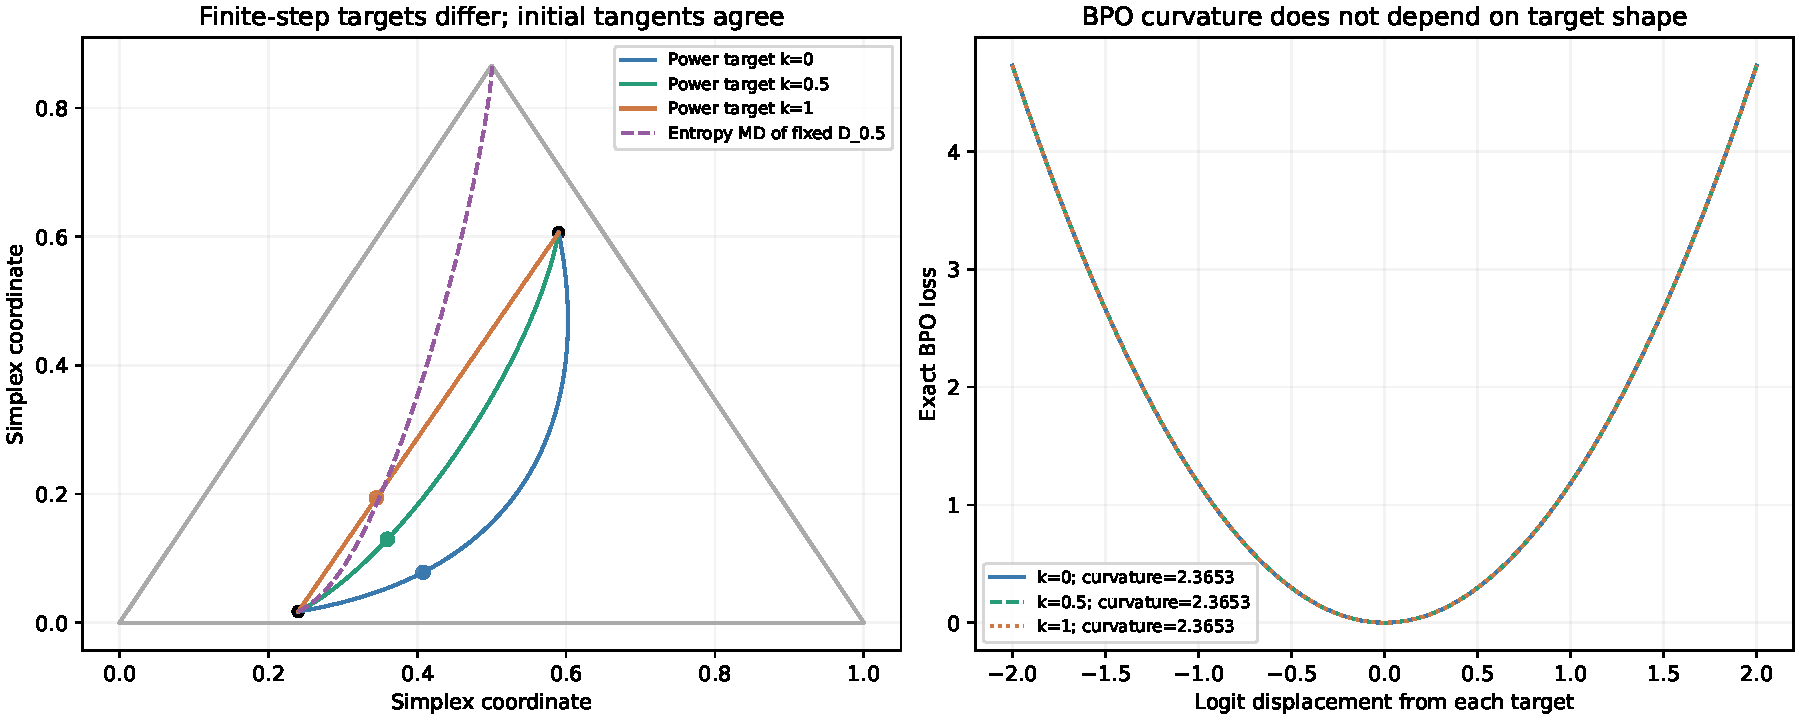
\includegraphics[width=\textwidth]{../../results/power-bpo-algorithm/geometry-and-curvature.pdf}
 \caption{左：幂均值有限步路径与固定 $D_{1/2}$ 的 entropy MD 路径只有起始切向量一致。右：不同 target 只平移固定 $q,\eta$ 的 BPO 二次损失，曲率不随 $\kappa$ 改变。}
\end{figure}


\section{教师监督的方差与误差控制}
\label{sec:proximal-teacher-center}
\subsection{固定插值强度的统一二阶矩界}

本节先给所有 $0<\kappa\le1$、$0<\eta<1$ 都适用的上界，再分析小 $\eta$ 时的锐阶数。记未归一化信号为 $f_{\kappa,\eta}(r)=\kappa^{-1}\log(1-\eta+\eta e^{\kappa r})$，BPO 教师监督为 $A=f/\eta$。关于 $f$ 的二阶矩不能省去这一次 $1/\eta^2$ 缩放后直接称为 BPO 梯度方差。

\begin{theorem}[幂均值信号的统一二阶矩界]
\label{thm:proximal-power-variance}
有限词表上 $q_a,T_a>0$，$0<\kappa\le1$、$0<\eta<1$。令
\begin{equation}
 C_\star=\sup_{u>0}\frac{\log^2(1+u)}u<\infty,\qquad
 B_{\kappa,\eta}=\frac{\log^2(1-\eta)+C_\star\eta}{\kappa^2}.
\end{equation}
则 $\E_qf^2\le B_{\kappa,\eta}$、$\E_qA^2\le B_{\kappa,\eta}/\eta^2$。若 $\|\psi(a)\|\le S$，有
\begin{equation}
 \Var_q[\psi C_qA]\le S^2\Var_qA
 \le S^2B_{\kappa,\eta}/\eta^2.
\end{equation}
该界不依赖词表维数。对 $\kappa=0$，一般不存在有限分布无关上界。
\end{theorem}

\begin{proof}
记 $\rho=T/q$。在 $\rho<1$ 上，$\log(1-\eta)/\kappa\le f<0$，负区域二阶矩不超过 $\log^2(1-\eta)/\kappa^2$。在 $\rho\ge1$ 上，
\begin{equation}
 0\le f\le\kappa^{-1}\log(1+\eta\rho^\kappa),\qquad
 f^2\le C_\star\eta\rho^\kappa/\kappa^2.
\end{equation}
由 $x^\kappa$ 的凹性与 $\E_q\rho=1$，有 $\E_q\rho^\kappa\le1$。合并两个区域得到 $\E_qf^2$ 上界；$A=f/\eta$ 给出监督的上界。常数有限，因为 $\log^2(1+u)/u$ 在零处和无穷处都趋零，在中间连续。梯度协方差 trace 不超过其二阶矩，而 $\E_q\|\psi C_qA\|^2\le S^2\Var_qA$。几何端点的发散由第~\ref{sec:power-setup}~节的二元反例给出。
\end{proof}

\subsection{平方根形状的有界自然梯度与显式动力学}

由式~\eqref{eq:proximal-natural-velocity}，$\|v_\kappa\|_F^2=\Var_q(\rho^\kappa)/\kappa^2$。当 $0<\kappa\le1/2$，$2\kappa\le1$，Jensen 不等式给出 $\E_q\rho^{2\kappa}\le(\E_q\rho)^{2\kappa}=1$，于是
\begin{equation}
 \|v_\kappa\|_F^2\le\frac{1-A_\kappa^2}{\kappa^2}\le\frac1{\kappa^2}.
 \label{eq:proximal-natural-speed-bound}
\end{equation}
该界对任意完整支持的 $q,t$ 成立，不需要给 teacher 或 student 指定统一概率下界。对于 $\kappa>1/2$，取 $q=(\varepsilon,1-\varepsilon)$、$t=(c,1-c)$，$0<c<1$ 固定，则
\begin{equation}
 \Var_q(\rho^\kappa)
 =\varepsilon(1-\varepsilon)
 \left[(c/\varepsilon)^\kappa-((1-c)/(1-\varepsilon))^\kappa\right]^2
 \sim c^{2\kappa}\varepsilon^{1-2\kappa}\longrightarrow\infty.
\end{equation}
几何端点 $\kappa=0$ 也没有统一界：固定 $q=(1/4,3/4)$、令 $t=(\varepsilon,1-\varepsilon)$，$\Var_q\log(t/q)$ 随 $\varepsilon\to0$ 发散。故 $0<\kappa\le1/2$ 是这个自然梯度族具有统一 Fisher 速度界的区间。确定性的 Fisher 速度与随机参数梯度方差是不同对象，不能把这个结论直接写成完整训练梯度的方差定理。

在平方根点 $\kappa=1/2$，$A=\sum\sqrt{qt}$，并有 $\E_q\rho=1$，因此
\begin{equation}
 \|v_{1/2}\|_F^2=4(1-A^2)\le4,\qquad
 D_{1/2}(t\Vert q)=4(1-A).
\end{equation}
由 Lyapunov 等式，连续流满足
\begin{equation}
 \frac{dA}{d\tau}=1-A^2,
 \qquad A(\tau)=\tanh(\tau+\operatorname{artanh}A(0)),\quad q\ne t.
 \label{eq:proximal-hellinger-flow}
\end{equation}
证明是 $dD_{1/2}/d\tau=-4\,dA/d\tau=-4(1-A^2)$，然后积分 $dA/(1-A^2)=d\tau$。$q=t$ 时 $A=1$ 且流恒定。进一步，$D'=-(1+A)D$，由于 $0<A\le1$，有
\begin{equation}
 D(0)e^{-2\tau}\le D(\tau)\le D(0)e^{-\tau}.
\end{equation}
若写 $A=\cos\vartheta$，则 $d\vartheta/d\tau=-\sin\vartheta$。平方根形状既有球面解释，也有显式 teacher 接近度和有界 Fisher 速度。这使它成为一个有数学依据的候选点，尚不能据此断言其训练性能优于其他形状。

\begin{figure}[htbp]
 \centering
 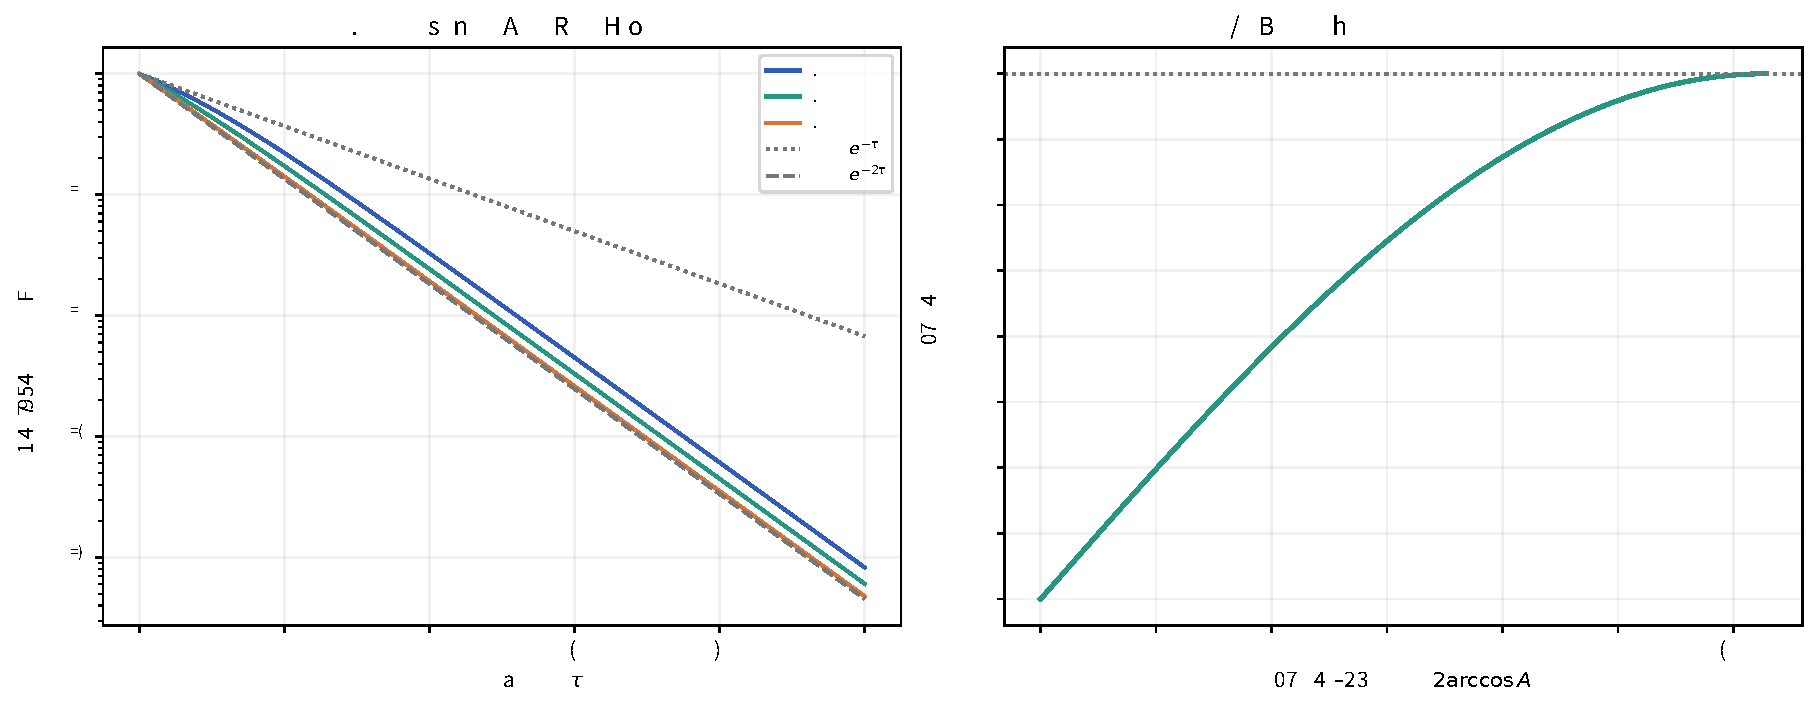
\includegraphics[width=\textwidth]{../../results/proximal-family-geometry/hellinger-flow.pdf}
 \caption{平方根形状的连续动力学。左图由 $A(\tau)=\tanh(\tau+\operatorname{artanh}A(0))$ 精确生成，归一化散度位于两个指数包络之间；右图将 Fisher 速度写成到 teacher 的 Fisher--Rao 距离函数，展示统一上界 2。}
\end{figure}

\subsection{小插值强度的最坏二阶矩存在形状阈值}

固定 $\kappa>0$ 时，上节使用的统一 $O(\lambda)$ 界还可以加强。这里考察完整支持概率分布上的最坏即时信号二阶矩
\begin{equation}
 \mathcal B_\kappa(\lambda)
 =\sup_{q,t}\E_q\left[
 \left(\frac1\kappa\log(1-\lambda+\lambda(t/q)^\kappa)\right)^2
 \right].
\end{equation}
上界对任何有限维数成立；下界的二元见证已足够。它是未标准化的冻结信号，不含 student 残差。

\begin{theorem}[最坏二阶矩的精确小强度阶数]
\label{thm:proximal-moment-threshold}
对任意固定 $0<\kappa\le1$，当 $\lambda\to0$ 时
\begin{equation}
 \mathcal B_\kappa(\lambda)=\Theta_\kappa\left(\lambda^{\min\{2,1/\kappa\}}\right).
 \label{eq:proximal-sharp-moment-order}
\end{equation}
$\Theta_\kappa$ 中的常数可依赖 $\kappa$，不依赖词表维数。几何端点则满足 $\mathcal B_0(\lambda)=\infty$，对任意 $\lambda>0$ 成立。
\end{theorem}

\begin{proof}
记 $\rho=t/q$。负区域 $\rho<1$ 的二阶矩不超过 $\log^2(1-\lambda)/\kappa^2=O_\kappa(\lambda^2)$。在正区域，$0\le f\le\log(1+\lambda\rho^\kappa)/\kappa$。

若 $0<\kappa\le1/2$，用 $\log(1+x)\le x$ 与 $\E_q\rho^{2\kappa}\le1$ 得到
\begin{equation}
 \E_q[f^2\mathbf1\{\rho\ge1\}]
 \le\frac{\lambda^2}{\kappa^2}\E_q\rho^{2\kappa}
 \le\frac{\lambda^2}{\kappa^2}.
\end{equation}
所以 $\mathcal B_\kappa(\lambda)\le[\log^2(1-\lambda)+\lambda^2]/\kappa^2=O_\kappa(\lambda^2)$。取任一固定完整支持且 $q\ne t$ 的二元分布，逐项 Taylor 展开给出 $f/\lambda\to(\rho^\kappa-1)/\kappa$。有限项求和后 $\E_qf^2/\lambda^2\to\E_q(\rho^\kappa-1)^2/\kappa^2>0$，得到匹配的下界。

若 $1/2<\kappa\le1$，令 $s=1/\kappa\in[1,2)$。常数 $C_s=\sup_{x>0}\log^2(1+x)/x^s$ 有限，因为比值在零点按 $x^{2-s}$ 趋零，在无穷处也趋零。于是
\begin{equation}
 \E_q[f^2\mathbf1\{\rho\ge1\}]
 \le\frac{C_s\lambda^s}{\kappa^2}\E_q\rho^{\kappa s}
 =\frac{C_s\lambda^{1/\kappa}}{\kappa^2}.
\end{equation}
负区域的 $O(\lambda^2)$ 比这个阶数更小。为证明下界，取 $t=(1/2,1/2)$、$q_1=\tfrac12\lambda^{1/\kappa}$、$q_2=1-q_1$。第一项满足 $\rho_1=\lambda^{-1/\kappa}$、$f_1=\log(2-\lambda)/\kappa$，所以
\begin{equation}
 \E_qf^2\ge q_1f_1^2
 =\frac{\lambda^{1/\kappa}}{2\kappa^2}\log^2(2-\lambda)
 =\Omega_\kappa(\lambda^{1/\kappa}).
\end{equation}
上下界匹配。$\kappa=1/2$ 已由第一种情况覆盖，也可取 $s=2$、$C_2=1$。$\kappa=0$ 时 $f=\lambda\log(t/q)$，固定有正质量的 $q$ 并令对应 teacher 概率趋零，二阶矩无界。\hfill$\square$
\end{proof}

这个阶数区分了“固定分布的小步展开”与“对所有分布统一的小步上界”。固定 $q,t$ 时，对每个 $\kappa$ 都有 $\E_qf^2=O(\lambda^2)$；最坏情形允许 $q,t$ 随 $\lambda$ 改变，$\kappa>1/2$ 的稀有正尾部因此留下更慢的 $\lambda^{1/\kappa}$ 阶数。TOP-D 算术端点为 $\Theta(\lambda)$，平方根点为 $\Theta(\lambda^2)$，二者的差异来自采样二阶矩，不是两种学习率单位。

若 score 范数不超过 $M$，定理立即给即时 score 估计与精确条件中心化估计相同阶数的方差上界，因为 $\Var(\psi f)\le M^2\E_qf^2$、$\Var(\psi C_qf)\le M^2\E_qf^2$。它没有证明所有参数化模型都达到这个最坏阶数，也没有覆盖随机标准化后的信号。

\begin{figure}[htbp]
 \centering
 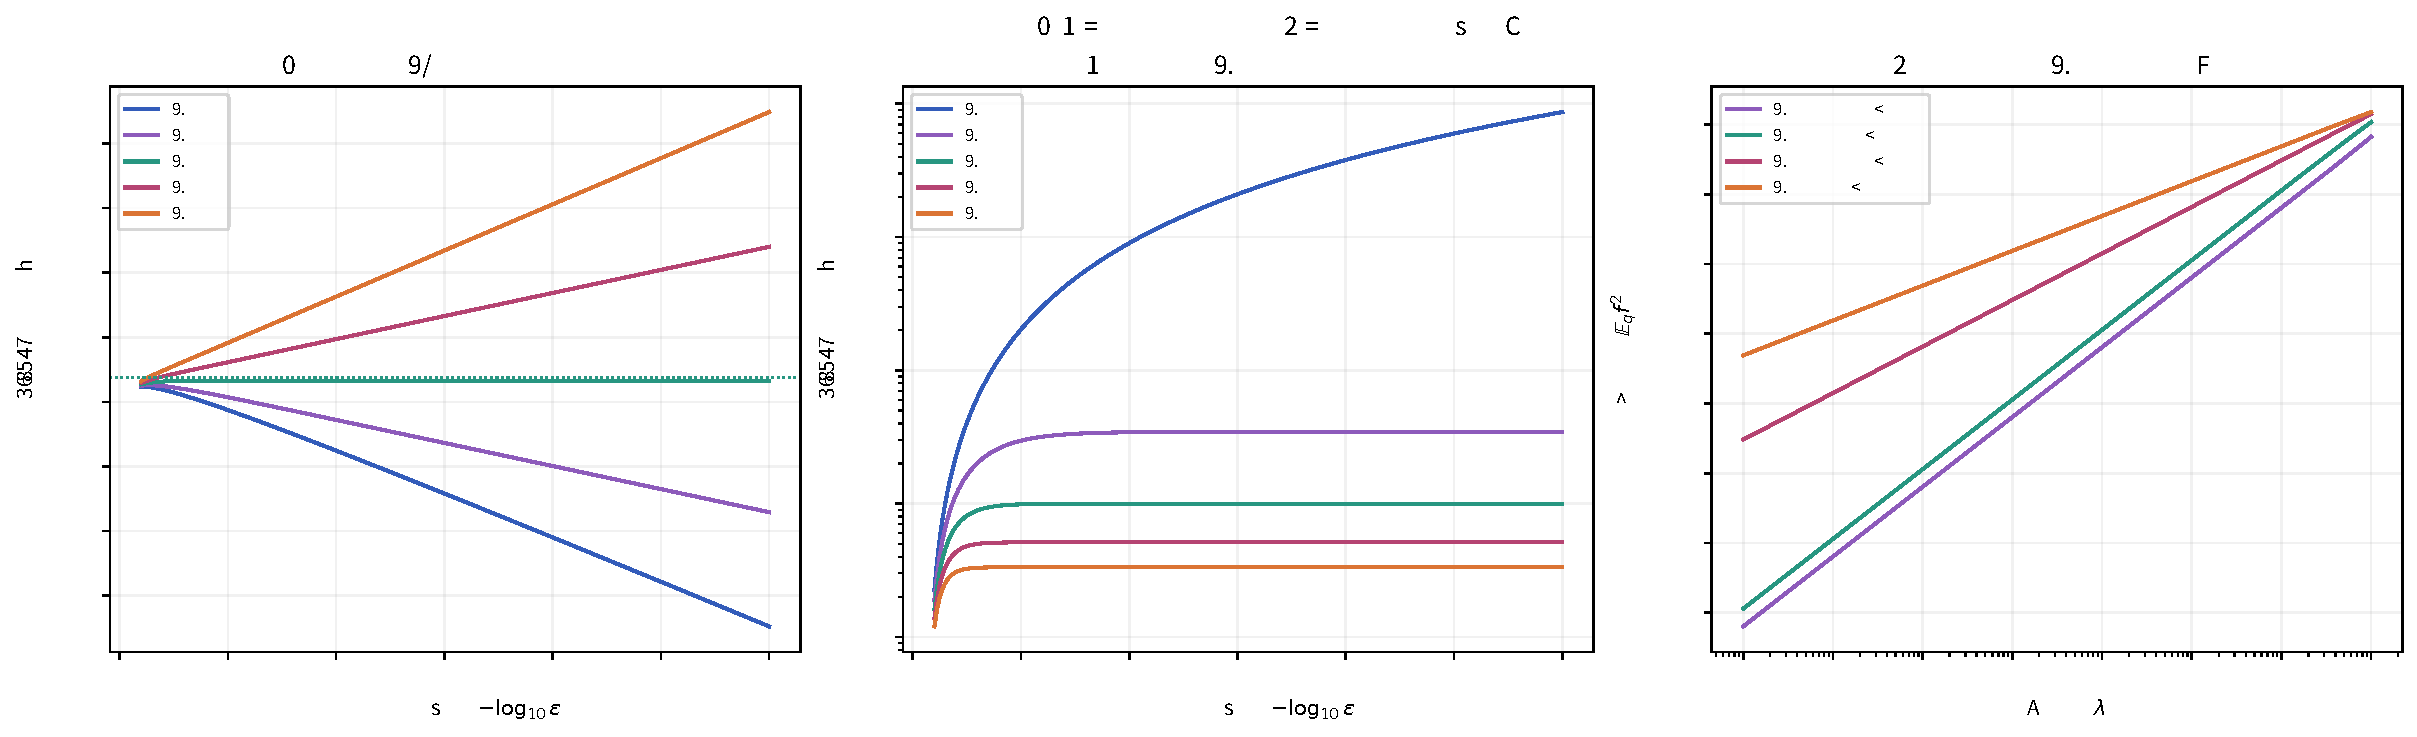
\includegraphics[width=\textwidth]{../../results/proximal-family-geometry/threshold.pdf}
 \caption{形状阈值的解析见证。左图让学生概率趋零，$\kappa>1/2$ 的自然梯度 Fisher 速度发散；中图让 teacher 概率趋零，几何端点的速度发散；右图使用随 $\lambda$ 改变的二元 anchor，信号二阶矩斜率分别趋于 $2,2,4/3,1$。右图不是对所有分布做数值最大化，其作用是验证证明中的下界见证。}
\end{figure}

\subsection{共享参数子流形上的自然梯度投影}

独立 token 分布的速度界还可延伸到共享参数的自然梯度流，但需要明确度量。取有限个 prefix、固定权重 $d_s>0$、$\sum_sd_s=1$，将外层分布写成 $q_\theta(a\mid s)>0$。定义
\begin{equation}
 L_\kappa(\theta)=\sum_sd_sD_\kappa(t_s\Vert q_{\theta,s}),\qquad
 \langle v,w\rangle_W=\sum_{s,a}\frac{d_s}{q_{\theta,s,a}}v_{s,a}w_{s,a}.
\end{equation}
记 $J=\partial q_\theta/\partial\theta$，$W=\operatorname{diag}(d_s/q_{\theta,s,a})$，则参数 Fisher 矩阵为 $\mathcal I=J^\top WJ$。令 $v$ 为每个 prefix 上的无约束负自然梯度，$v_{s,a}=q_{\theta,s,a}(\rho_{s,a}^\kappa-\E_{q_{\theta,s}}\rho_s^\kappa)/\kappa$。因为每个 prefix 的 $J$ 列向量分量和为零，$\nabla_\theta L=-J^\top Wv$。

参数自然梯度流采用 Moore--Penrose 广义逆 $\mathcal I^+$ 时，有
\begin{equation}
 \dot\theta=-\mathcal I^+\nabla_\theta L,\qquad
 \dot q_\theta=J\mathcal I^+J^\top Wv=Pv.
\end{equation}
$P$ 是到 $\operatorname{range}(J)$ 的 $W$ 正交投影：令 $B=W^{1/2}J$，则 $W^{1/2}PW^{-1/2}=B(B^\top B)^+B^\top$，后者是普通欧氏正交投影。因此
\begin{equation}
 \|\dot q_\theta\|_W^2\le\|v\|_W^2,\qquad
 \frac{dL}{d\tau}=-\langle v,Pv\rangle_W=-\|Pv\|_W^2\le0.
\end{equation}
平方根形状满足 $\|v\|_W^2=\sum_sd_s\,4(1-A_s^2)\le4$，所以共享参数的精确自然梯度流也满足 $\|\dot q_\theta\|_W\le2$。更一般地，$0<\kappa\le1/2$ 时平方速度不超过 $1/\kappa^2$。

这个结论控制的是分布流在固定 prefix Fisher 度量下的速度。它不控制参数的欧氏范数，也不自动适用于普通梯度流。共享参数还可能使 $Pv=0$ 而 $q_\theta\ne t$，因此单调性和速度界并不保证无投影误差的 teacher 收敛。离散幂均值 target 的精确 escort 轨迹也不会因这个局部投影结论自动延续到共享参数模型。

\subsection{平方根候选与尚待回答的数学问题}

三个独立结果支持优先研究 $\kappa=1/2$：它是 Hellinger 重心并沿 Fisher--Rao 短弧；连续流有显式 $A(\tau)$ 和 $\|v\|_F\le2$；小 $\lambda$ 的统一即时信号二阶矩为 $O(\lambda^2)$。$0<\kappa<1/2$ 也具有有界速度和相同最坏阶数，但上界常数、目标路径与 teacher 散度不同。$\kappa=1/2$ 是仍具有这两个统一矩性质的最大形状参数，尚不是在任何固定任务损失下证明的最优形状。

在 $0<\kappa\le1/2$ 内，所给速度平方上界 $1/\kappa^2$ 与信号二阶矩上界 $[\log^2(1-\lambda)+\lambda^2]/\kappa^2$ 都随 $\kappa$ 增大而减小，负信号下界 $\log(1-\lambda)/\kappa$ 则增大。平方根点在这一组统一界上有最小的上界和最温和的负下界。界的优劣不等于每个固定分布上的实际方差优劣，不能把这段比较替代固定评价目标下的最优性证明。

下一步的纯数学工作应区分目标选择与模型投影。固定一个外部评价散度后，研究不同 $\kappa$ 的有限步改进、曲率与噪声常数，才有可比较的优化问题；直接最小化各自不同的 $D_\kappa$ 数值不能给出通用最优 $\kappa$。共享参数策略族下，还需证明有限 inner 的拟合损失怎样控制 $D_\kappa(m\Vert p)$ 或 escort 误差，才能把精确外层结论应用到模型更新；上一小节的自然梯度投影只提供连续时间单调性和速度界。prefix 测度刷新是另一项独立条件。

新增图和精确求和核验由 \path{experiments/analysis/proximal_family_dynamics.py} 生成，数据和版本见 \path{results/proximal-family-geometry/dynamics-summary.json}。3、64、1024 维各五组随机概率向量检验超额损失分解、teacher 进展恒等式、escort 步和自然梯度流；有限差分另检验最优点的 Hessian 与 escort 流导数。共享参数核验使用三个 prefix、每个五个 action、四个共享参数的条件指数族，验证参数梯度、Fisher 正交投影和速度界。幂均值、原始散度和新的核验结论均保留完整支持条件。

\subsection{幂均值教师中心、advantage 与可认证估计}
\label{sec:proximal-teacher-center}

本小节继续采用前节的单教师 BPO：固定前缀和完整正支持 $q,T$，记 $\rho=T/q$、$0\le\kappa\le1$、$0<\eta<1$。冻结教师信号、教师中心和中心化 advantage 分别为
\begin{align}
 A_{\kappa,\eta}(a)&=\begin{cases}
 \log\rho_a,&\kappa=0,\\
 (\kappa\eta)^{-1}\log(1-\eta+\eta\rho_a^\kappa),&\kappa>0,
 \end{cases}\\
 K_{\kappa,\eta}&=-\sum_aq_a A_{\kappa,\eta}(a),\\
 B_{\kappa,\eta}(a)&=A_{\kappa,\eta}(a)+K_{\kappa,\eta},\qquad \E_qB=0.
 \label{eq:center-explicit-definition}
\end{align}
当前 $K$ 已经含有 $1/\eta$。若缓存原始信号中心 $\widetilde K=-\E_qf$，则 $\widetilde K=\eta K$，在 BPO 系数中只除以 $\eta$ 一次。

$B$ 是条件中心化的教师监督，不是跨 response 的组 advantage。$A$、$K$ 在本轮 inner 中冻结；学生反馈 $C_qU/\eta$ 随参数改变。

\subsubsection{完整展开、KL 端点与凸散度表示}

几何端点恢复
\begin{equation}
 K_{0,\eta}=\sum_aq_a\log(q_a/T_a)=\KL(q\Vert T).
\end{equation}
一般形状则为
\begin{equation}
 \boxed{K_{\kappa,\eta}
 =-\frac1{\kappa\eta}\sum_aq_a
 \log\left(1-\eta+\eta(T_a/q_a)^\kappa\right).}
 \label{eq:center-expanded-k}
\end{equation}
算术端点满足
\begin{equation}
 K_{1,\eta}=\eta^{-1}\KL\big(q\Vert(1-\eta)q+\eta T\big).
\end{equation}
一般 $\kappa$ 下，若 $m$ 是归一化幂均值 target、$Z=\sum_aq_ae^{f_a}$，则
\begin{equation}
 K_{\kappa,\eta}=\frac{\KL(q\Vert m)-\log Z}{\eta}.
\end{equation}
所以不能把它继续标为原 teacher KL。

然而 $K$ 本身是一个合法的凸 $f$-divergence。定义
\begin{equation}
 \phi_{\kappa,\eta}(x)=x-1-
 \frac{\log(1-\eta+\eta x^\kappa)}{\kappa\eta},\qquad x>0.
 \label{eq:center-convex-generator}
\end{equation}
它满足 $\phi(1)=\phi'(1)=0$，且
\begin{equation}
 \phi''(x)=
 \frac{x^{\kappa-2}[(1-\kappa)(1-\eta)+\eta x^\kappa]}
 {(1-\eta+\eta x^\kappa)^2}>0.
\end{equation}
因此 $\phi(x)\ge0$，再由 $\E_q(\rho-1)=0$，得到
\begin{equation}
 K_{\kappa,\eta}=\E_q\phi_{\kappa,\eta}(T/q).
\end{equation}
这个式子的标准 $f$-divergence 参照测度是 $q$，第一分布是 $T$；其生成函数包含 $\kappa,\eta$。几何极限为 $\phi_0(x)=x-1-\log x$。它与普通 KL 或前文 $D_\kappa$ 的关系由上述端点和极限决定，不能因其非负就把名称混用。

\subsubsection{中心的有界性、单调性与小步极限}

\begin{theorem}[教师中心的分布无关界]
\label{thm:center-bounds-monotonicity}
令 $0<\kappa\le1$、$0<\eta<1$，则
\begin{equation}
 0\le K_{\kappa,\eta}
 \le\min\left\{\KL(q\Vert T),\;
 c_{\kappa,\eta}\right\},\qquad
 c_{\kappa,\eta}=-\frac{\log(1-\eta)}{\kappa\eta}.
 \label{eq:center-uniform-cap}
\end{equation}
$K=0$ 当且仅当 $q=T$。固定 $q,T$ 时，$K$ 随 $\kappa$ 非增加、随 $\eta$ 非减少。对任意至少二元的词表，上界 $c_{\kappa,\eta}$ 是对完整支持分布取上确界的锐值。
\end{theorem}

\begin{proof}
凸生成函数给出非负性和零点唯一性。逐 action 有 $A\ge\log(1-\eta)/(\kappa\eta)=-c$，取负均值得到 $K\le c$。加权 AM--GM 不等式给出 $1-\eta+\eta\rho^\kappa\ge\rho^{\kappa\eta}$，故 $A\ge\log\rho$，得到 $K\le\KL(q\Vert T)$。

固定 $r=\log\rho$，令 $H(k)=\log(1-\eta+\eta e^{kr})$。$H(0)=0$ 且
\begin{equation}
 H''(k)=\frac{\eta(1-\eta)r^2e^{kr}}{(1-\eta+\eta e^{kr})^2}\ge0.
\end{equation}
凸函数从零点出发的割线斜率 $H(k)/k$ 非减少，因此 $A=H(k)/(k\eta)$ 随 $k$ 非减少，$K$ 非增加。

固定 $k>0$，记 $x=\rho^k-1>-1$、$y=1+\eta x>0$，则
\begin{equation}
 \partial_\eta A=\frac{1-y^{-1}-\log y}{k\eta^2}\le0,
\end{equation}
因为 $\log y-1+y^{-1}\ge0$。取负期望得到 $K$ 随 $\eta$ 非减少。

为证明锐性，取 $q=(\epsilon,1-\epsilon)$、$T=(1-\epsilon^2,\epsilon^2)$，$\epsilon\to0$。常见 action 的比率趋零，$-A\to c$；稀有 action 对 $K$ 的贡献为 $O(\epsilon\log\epsilon)$，趋零。因此 $K\to c$。所有有限 $\epsilon>0$ 都保持完整支持。\hfill$\square$
\end{proof}

该上界控制的是新的鲁棒散度，不是原 teacher KL 的上界；$K$ 有界并不意味着 $\KL(q\Vert T)$ 有界。作为固定参数的凸散度，$K$ 可以继承前节理想 teacher 保持路径的数据处理性质，但训练中缓存的 $K(q_n,T)$ 在整个 inner 窗口本来就是常数，不能把它当成不断变化的拟合误差。

当 $\eta=1$ 时全部形状恢复 $A=\log\rho$、$K=\KL(q\Vert T)$，不再具有上面的有限分布无关上界。当 $\kappa\to0$ 时上界也发散；原 KL 没有自动获得有界性。

对固定完整支持 $q,T$，Taylor 展开给出
\begin{align}
 A_{\kappa,\eta}&\longrightarrow\frac{\rho^\kappa-1}{\kappa},\\
 K_{\kappa,\eta}&\longrightarrow
 \frac{1-a_\kappa}{\kappa},\qquad
 a_\kappa=\sum_aq_a^{1-\kappa}T_a^\kappa.
 \label{eq:center-small-step-limit}
\end{align}
$0<\kappa<1$ 时此极限是 $(1-\kappa)D_\kappa(T\Vert q)$；$\kappa=1$ 的极限为零。由 $\log(1+\eta x)\le\eta x$，这个极限同时给出有限 $\eta$ 的下界 $K\ge(1-a_\kappa)/\kappa$。

平方根点尤其简单：
\begin{equation}
 \lim_{\eta\to0}K_{1/2,\eta}
 =2\left(1-\sum_a\sqrt{q_aT_a}\right)
 =\sum_a(\sqrt{q_a}-\sqrt{T_a})^2=:H^2(q,T)\le2.
\end{equation}
这里明确采用不带 $1/2$ 因子的平方 Hellinger 距离。

当 $\rho=1+\delta$ 且全部比率一致接近一时，生成函数在一附近展开为
\begin{equation}
 K_{\kappa,\eta}
 =\frac{1-\kappa(1-\eta)}2\chi^2(T\Vert q)
  +O(\E_q|\delta|^3).
\end{equation}
这描述局部教师差异；对任意极端概率比不能使用这个 Taylor 余项作统一保证。

\subsubsection{Advantage 的单侧界与误差相关方差界}

精确中心化不改变标量方差：
\begin{equation}
 V_{\kappa,\eta}:=\Var_q(B)=\Var_q(A).
\end{equation}
因此 $K$ 使均值归零，但标量方差的改变来自 $A$ 的形状变换。 这里限定为固定 prefix。跨冻结状态测度 $d$ 的总方差满足
\begin{align}
 \Var_{d,q}(A)&=\E_dV_s+\Var_d(K_s),\\
 \Var_{d,q}(B)&=\E_dV_s.
\end{align}
因此按 prefix 精确中心化会移除不同 prefix 的监督均值差异，$\kappa=0$ 也有这项标量收益；它不等于降低条件 action 方差，也不自动降低带 score 权重的参数梯度方差。

由前面的逐 action 下界，
\begin{equation}
 B(a)\ge K_{\kappa,\eta}-c_{\kappa,\eta}\ge-c_{\kappa,\eta}.
\end{equation}
没有不依赖 $q,T$ 的逐 action 正上界：当 $q_a\to0$ 而 $T_a$ 保持正质量，$A_a$ 按 $\log(T_a/q_a)/\eta$ 增长。单侧有界、方差有界与双侧有界是不同结论。

对任何固定 $\kappa>0,\eta<1$，仍然存在统一的有限方差界。在 $A>0$ 区域，$A\le\log\rho/\eta$；Markov 不等式与 $\E_q\rho=1$ 给出 $\Pr(A>x)\le e^{-\eta x}$、$x\ge0$。因此
\begin{equation}
 V\le\E_qA^2\le c_{\kappa,\eta}^2+2/\eta^2.
\end{equation}
下面的平方根阈值涉及 $\eta\to0$ 时能否保持常数级统一界，不表示较大 $\kappa$ 在固定正 $\eta$ 下完全没有方差界。

\begin{theorem}[中心化教师 advantage 的方差控制]
\label{thm:center-advantage-variance}
若 $0<\kappa\le1/2$、$0<\eta<1$，则
\begin{align}
 V_{\kappa,\eta}
 &\le\frac{1-a_\kappa^2}{\kappa^2(1-\eta)^2}
 \le\frac1{\kappa^2(1-\eta)^2},\\
 V_{\kappa,\eta}
 &\le\frac{2}{\kappa(1-\eta)^2}K_{\kappa,\eta}.
 \label{eq:center-error-scaled-variance}
\end{align}
这两个界均不依赖词表维数或概率的统一正下界。
\end{theorem}

\begin{proof}
令 $X=\rho^\kappa$、$h(X)=\log(1-\eta+\eta X)/(\kappa\eta)$。对 $X\ge0$，$|h'|\le1/[\kappa(1-\eta)]$。若 $X'$ 是独立同分布副本，方差的成对表示给出
\begin{equation}
 \Var h(X)=\frac12\E(h(X)-h(X'))^2
 \le\frac{\Var X}{\kappa^2(1-\eta)^2}.
\end{equation}
由于 $2\kappa\le1$，Jensen 不等式给出 $\E_q\rho^{2\kappa}\le(\E_q\rho)^{2\kappa}=1$，因此 $\Var X\le1-a_\kappa^2$。又由 $K\ge(1-a_\kappa)/\kappa$、$1+a_\kappa\le2$，
\begin{equation}
 \frac{1-a_\kappa^2}{\kappa^2(1-\eta)^2}
 =\frac{(1+a_\kappa)(1-a_\kappa)}{\kappa^2(1-\eta)^2}
 \le\frac{2K}{\kappa(1-\eta)^2}.
\end{equation}
\hfill$\square$
\end{proof}

在 inner 起点，若 score 范数不超过 $M$，teacher score 抽样满足 $\Var(g)\le\E\|g\|^2\le M^2V\le2M^2K/[\kappa(1-\eta)^2]$。这是带 score 条件的误差相关噪声界，不是全模型无条件性质。

平方根点有 $V\le4K/(1-\eta)^2$，并在小步极限得到精确关系
\begin{equation}
 \lim_{\eta\to0}V_{1/2,\eta}
 =4(1-a_{1/2}^2)=H^2(4-H^2)\le4.
\end{equation}
因此该极限的教师中心与 advantage 方差同时有界，且教师差异趋零时方差也趋零。

前面的原始信号锐矩阶数还能加强为中心化后的结论：对固定 $0<\kappa\le1$，
\begin{equation}
 \sup_{q,T}V_{\kappa,\eta}
 =\Theta_\kappa\big(\eta^{\min\{2,1/\kappa\}-2}\big),\qquad\eta\to0.
\end{equation}
上界由 $\Var A\le\E A^2$ 和定理~\ref{thm:proximal-moment-threshold} 得到。$\kappa\le1/2$ 的下界取任一固定非同分布 $q,T$，小步极限的方差严格为正。$\kappa>1/2$ 时取 $q_1=\eta^{1/\kappa}/2$、$T_1=1/2$，则 $A_1=\log(2-\eta)/(\kappa\eta)$，而 $A_2$ 保持有限；二元方差 $q_1q_2(A_1-A_2)^2$ 给出匹配的下界。$\kappa=0$ 则对任意 $\eta$ 都无统一方差上界。这里允许最坏分布随 $\eta$ 改变，不能混同于固定分布上的连续极限。

更精确地，记前文锐 Fisher 速度常数为 $C_{\mathrm{vel}}(\kappa)=\sup_{q,T}\Var_q(\rho^\kappa)/\kappa^2$。上述 Lipschitz 证明给出 $V\le C_{\mathrm{vel}}/(1-\eta)^2$，而任意固定正支持分布的极限是 $\Var_q(\rho^\kappa)/\kappa^2$。先选择逼近上确界的固定分布、再令 $\eta\to0$，上下界夹逼得到
\begin{equation}
 \lim_{\eta\to0}\sup_{q,T}V_{\kappa,\eta}
 =C_{\mathrm{vel}}(\kappa),\qquad0<\kappa\le1/2.
\end{equation}
所以前文 $\kappa_\star=0.4419283735$ 也最小化最坏的小步标量 advantage 方差，其锐值为 $3.5272748442$；平方根点的值为 4。这个准则不是全参数梯度信噪比，也不是数学任务正确率。 几何端点甚至不能仅从 KL 小推出低方差：取 $q=(\epsilon,1-\epsilon)$、$T=(e^{-\epsilon^{-3/4}},1-e^{-\epsilon^{-3/4}})$，则 $K_{0,\eta}\sim\epsilon^{1/4}\to0$，但 $\Var_qB_{0,\eta}\sim\epsilon^{-1/2}\to\infty$。固定正形状和固定 $\eta<1$ 的负尾部饱和会在同一族上使方差降至 $O(\epsilon)$。


\begin{figure}[htbp]
 \centering
 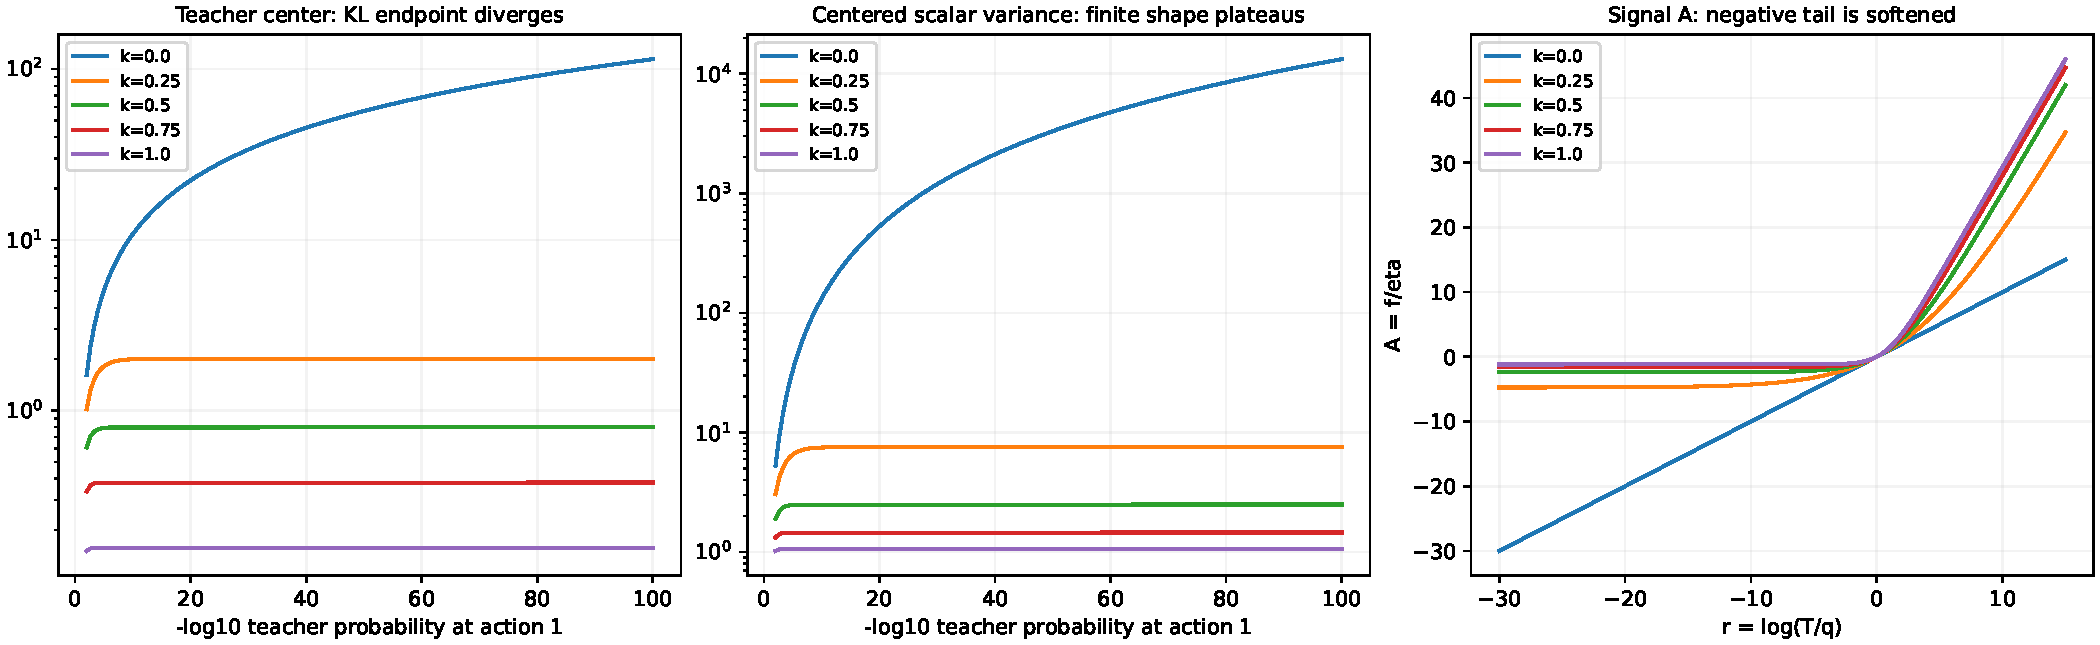
\includegraphics[width=\textwidth]{../../results/power-center-advantage/negative-tail-center-variance.pdf}
 \caption{固定 $q=(1/2,1/2)$、$\eta=0.3$，teacher 一个概率趋零时，几何中心及 advantage 方差发散，正形状出现平台。右图显示规范化信号 $A$ 的负尾部变化。曲线由完整二元分布精确求和生成。}
\end{figure}
\begin{figure}[htbp]
 \centering
 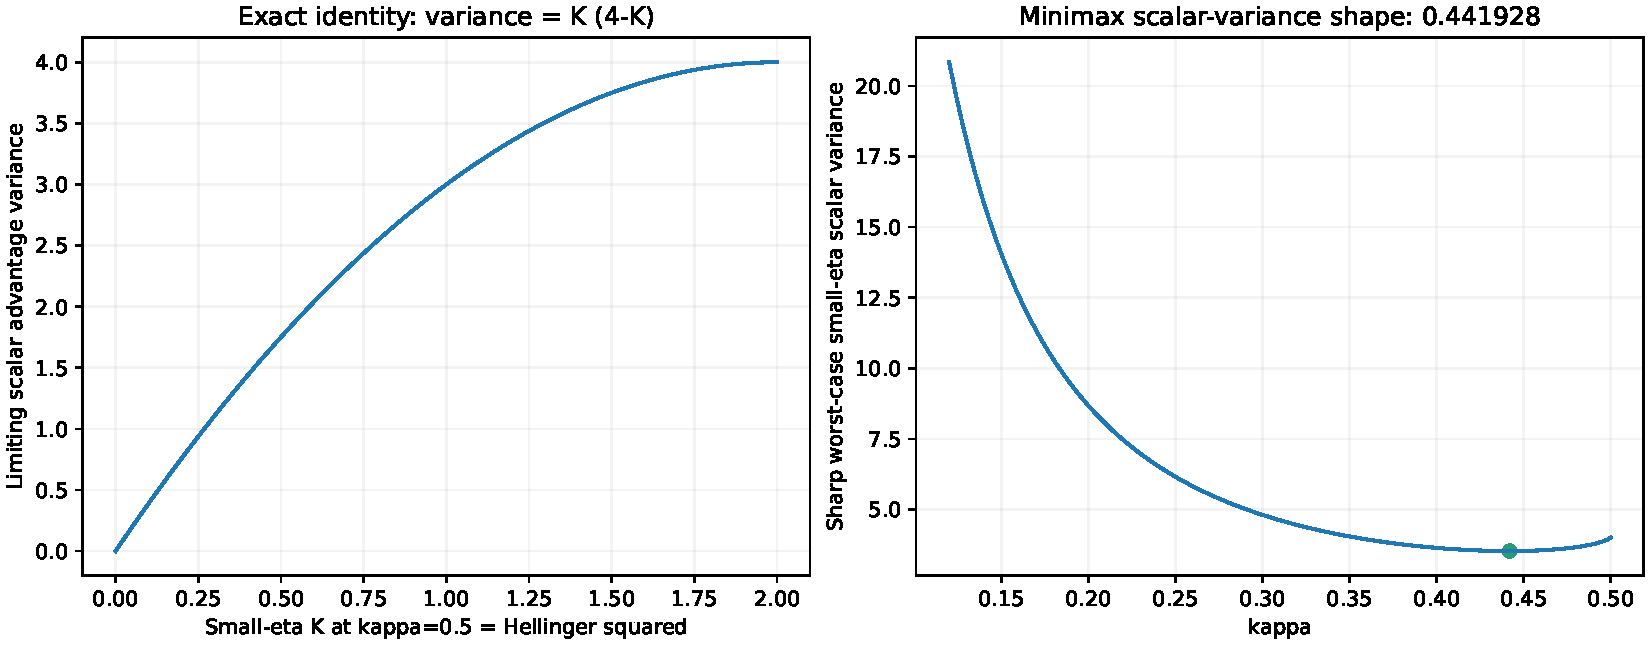
\includegraphics[width=\textwidth]{../../results/power-center-advantage/sharp-small-step-center-variance.pdf}
 \caption{左：平方根的小步极限满足 $V=K(4-K)$。右：最坏标量 advantage 方差的锐小步常数与前文自然速度常数一致，最优形状约为 $0.441928$。}
\end{figure}

\subsubsection{精确求和、Monte Carlo 与非负估计的代价}

若 teacher forward 能提供该前缀完整 logits，则使用完整 $q$ 权重直接求式~\eqref{eq:center-expanded-k}，不需要生成第二条 response。信号在 log 空间用 logaddexp 计算，避免先形成极大的 $T/q$。该中心可以按 prefix 缓存并冻结。

若采用独立 $a_i\sim q(\cdot\mid s)$，有无偏估计
\begin{equation}
 \widehat K=-\frac1M\sum_{i=1}^MA(a_i),\qquad
 \Var\widehat K=V/M.
\end{equation}
$\widehat K$ 单次可以为负；这不违背其非负期望。另一个逐样本非负无偏估计为
\begin{equation}
 \widehat K_+=\frac1M\sum_i[\rho(a_i)-1-A(a_i)].
\end{equation}
两者期望相同，方差一般不同。 它们在局部与最坏尾部上具有不同表现。若 $\rho=1+\epsilon h$、$\E_qh=0$ 且 $h$ 有界，令 $c_0=1-\kappa(1-\eta)$，则
\begin{align}
 -A&=-\epsilon h+\tfrac12c_0\epsilon^2h^2+O(\epsilon^3),\\
 \phi(\rho)&=\tfrac12c_0\epsilon^2h^2+O(\epsilon^3),\\
 \Var(-A)&=\epsilon^2\E_qh^2+O(\epsilon^3),\\
 \Var\phi(\rho)&=\tfrac14c_0^2\epsilon^4\Var_q(h^2)+O(\epsilon^5).
\end{align}
因此包括 $\kappa=0$ 在内，接近同分布时非负控制变量估计可把方差从二阶降至四阶；这需要概率比一致接近一，不能扩展到任意重尾输入。

取 $q=(\epsilon,1-\epsilon)$、$T=(1/2,1/2)$、固定 $\kappa>0,\eta<1$，原始估计方差按 $O(\epsilon\log^2(1/\epsilon))\to0$；非负估计的稀有项为 $\rho\sim1/(2\epsilon)$，其方差按 $1/(4\epsilon)$ 发散。这个 $\rho-1$ 控制变量保证非负性，却不能提供统一低方差保证。固定数据上也可能降低方差，应记录真实条件矩后判断。 即便原 KL 很小，也不能自动使用局部结论：取 $q=(\epsilon,1-\epsilon)$、$T=(\epsilon^{1/4},1-\epsilon^{1/4})$，有 $\KL(q\Vert T)\sim\epsilon^{1/4}\to0$，但非负估计的方差按 $\epsilon^{-1/2}$ 发散。概率比一致接近一比 KL 小更强。

如果独立中心估计与当前 action 独立，$\Var[A(a)+\widehat K]=V+V/M$。估计中心不会自动降低标量 advantage 方差。若中心与 advantage 使用同一组 $M$ 个 action，固定参数下
\begin{equation}
 \E\left[\frac1M\sum_i(A_i-\bar A)\psi_i\right]
 =\frac{M-1}{M}\operatorname{Cov}_q(A,\psi).
\end{equation}
这个恒等式由展开双重和得到：$M$ 个同索引项贡献 $\E A\psi$，$M(M-1)$ 个异索引项贡献 $\E A\E\psi$。$M=1$ 时更新为零。 若同一个 action 改用非负估计 $\widehat K_+=\rho-1-A$，则
\begin{equation}
 A(a)+\widehat K_+(a)=\rho_a-1,
\end{equation}
完全消掉 $\kappa,\eta$ 的教师信号形状。在 $p=q$ 时，该 score 更新的期望是 $\E_T\psi_q$，对应 forward-KL 的下降方向，而不是原 $\E_qB\psi_q$。中心估计本身无偏，不代表与当前 action 共享样本后的梯度无偏。

$M>1$ 可以使用独立中心、leave-one-out 或无偏样本协方差系数；它们要求同一 prefix 下的独立动作，不能用不同前缀的 token 直接代替。本研究的主 BPO 路线采用完整条件求和，不引入 response 组。

\subsubsection{有界非负无偏中心估计器}

$q$ 提案下的非负估计会出现重尾，但可以利用已有 $K$ 上界构造另一个提案。令 $\kappa>0,\eta<1$，$c=-\log(1-\eta)/(\kappa\eta)\ge1$。由 $A\ge-c$ 与 $\phi\ge0$，逐 action 有
\begin{equation}
 0\le q_a\phi(\rho_a)\le T_a+(c-1)q_a.
\end{equation}
右侧的总质量是 $c$，所以定义归一化包络提案
\begin{equation}
 \mu_c=(1-1/c)q+(1/c)T,\qquad
 Z(a)=\frac{q_a}{\mu_c(a)}\phi(\rho_a),\quad a\sim\mu_c.
 \label{eq:center-bounded-mixture-estimator}
\end{equation}
无需知道真实 $K$ 即可采样：以概率 $1/c$ 从教师抽一个 action，否则从锚点抽一个 action。它只估计本 prefix 的中心，不把 response rollout 改为这个提案，也不引入 response 组。

\begin{theorem}[中心估计的最小统一样本上界]
\label{thm:center-bounded-estimator}
上述估计器满足
\begin{equation}
 \E_{\mu_c}Z=K,\qquad0\le Z\le c,\qquad
 \Var_{\mu_c}Z\le K(c-K)\le c^2/4.
\end{equation}
对 $M$ 次独立抽样，$\widehat K_\mu=M^{-1}\sum_iZ_i$ 无偏、非负且不超过 $c$，其方差不超过 $K(c-K)/M$。所有分布上统一成立的无偏估计器样本上界不可能小于 $c$。
\end{theorem}

\begin{proof}
定义给出 $\E_\mu Z=\sum_aq_a\phi(\rho_a)=K$。包络不等式给出 $0\le Z\le c$，于是 $Z^2\le cZ$，取期望再减 $K^2$ 得到方差界。独立平均将方差除以 $M$。若任意无偏估计器总被常数 $b$ 上界约束，则 $K=\E\widehat K\le b$；而前面的正支持见证可以使 $K\to c$，故 $b\ge c$。这个最优性只作用于统一样本上界，不宣称该提案在每个固定分布上具有最小方差。\hfill$\square$
\end{proof}

Hoeffding 不等式还给出明确的置信界
\begin{equation}
 \Pr\{ |\widehat K_\mu-K|\ge\epsilon\}
 \le2\exp(-2M\epsilon^2/c^2).
\end{equation}
$\kappa=0$ 或 $\eta=1$ 的 KL 在分布类上无界，因此不能保持一个有限统一样本上界的无偏估计器。固定已知分布可以有有限界，不能与这个分布类结论混同。

平方根的小步极限尤为直观：$c\to2$、$\mu_c\to(q+T)/2$、$\phi(\rho)\to(\sqrt\rho-1)^2$，于是
\begin{equation}
 Z_0(a)=\frac{2(\sqrt{T_a}-\sqrt{q_a})^2}{T_a+q_a}\in[0,2],
 \qquad\E_{(q+T)/2}Z_0=H^2(q,T).
\end{equation}
记 $K_{\mathrm H}=H^2$，则 $\Var Z_0\le K_{\mathrm H}(2-K_{\mathrm H})$；而 $q$ 提案下的原始有符号中心估计在此极限具有方差 $K_{\mathrm H}(4-K_{\mathrm H})$。因此在每个固定完整支持分布对的平方根小步极限，包络估计方差至多为原始估计的一半。有限 $\eta$ 时不保证逐输入都优于原始有符号估计，真实条件矩仍需报告。 若当前 $q$ action 与 $M$ 个中心样本独立，则估计 advantage $\widehat B=A(a)+\widehat K_\mu$ 的方差为 $V+\Var Z/M$。平方根小步极限因此满足
\begin{align}
 \Var\widehat B
 &\le K_{\mathrm H}(4-K_{\mathrm H})
    +K_{\mathrm H}(2-K_{\mathrm H})/M\\
 &\le4+\frac1{M(M+1)}.
\end{align}
第二步在 $K_{\mathrm H}\in[0,2]$ 上最大化该凹二次式，驻点为 $(2M+1)/(M+1)$。一个独立辅助中心 action 即 $M=1$ 时，上界为 4.5；使用有符号 $q$ 中心估计的对应统一界为 8。这个结论作用于冻结 prefix 的教师标量 advantage，并要求独立性；它不涵盖学生反馈项或直接成为全参数梯度方差定理。


主 BPO 的完整条件求和无需这个辅助估计器。若使用它构造 sampled-action advantage，中心抽样仍须与当前 action 独立，或者给出相关性修正；有界中心估计不使 $A$ 的正尾部变为有界，也不自动解决整段 inner 的缓存误差。单样本中心只需本前缀辅助 action，不能把它解释为新增完整 response。

\subsubsection{有限 head 与尾部质量的中心区间}

令 $S$ 为任一保留 head，$\delta=\sum_{a\notin S}q_a$、$\tau_T=\sum_{a\notin S}T_a$，记 $K_S=-\sum_{a\in S}q_aA_a$。当 $\delta>0$，尾部的 $\rho$ 条件均值为 $\tau_T/\delta$。函数 $-A(\rho)$ 凸且不超过 $c$，由 Jensen 得到
\begin{equation}
 \boxed{K_S-\delta A(\tau_T/\delta)
 \le K\le K_S+\delta c_{\kappa,\eta}.}
 \label{eq:center-head-tail-interval}
\end{equation}
下界正是把尾部合并为一个 action 后的中心，亦为对应 $f$-divergence 的数据处理下界。区间宽度为 $\delta[c+A(\tau_T/\delta)]$，可直接计算；$\delta=0$ 时直接用完整 head 和。几何端点仍有 Jensen 下界，但没有仅靠两种尾部质量获得的有限统一上界。 对嵌套 head，拆分尾部由 Jensen 保证下界非减少；新增 action $a$ 对上界的改变量为 $q_a[-A_a-c]\le0$，所以上界非增加。可以持续扩大 head，直到区间宽度不超过 $\epsilon$，再取中点获得绝对中心误差不超过 $\epsilon/2$ 的确定性证书。

以一个已估计中心代替精确 $K$，会给 BPO score 系数加入常数误差 $\Delta K$。若 $\Delta K=\widehat K-K$，当前学生不等于 $q$ 时，梯度偏差为 $-\Delta K\E_q\psi_p$，若 $\|\psi_p\|\le M$，其范数不超过 $M|\Delta K|$。因此区间既报告中心误差，也能给固定参数下的 score 偏差提供证书。 这个偏差结论作用于停止系数并使用原始 $\psi_p$ 的 score 更新。若精确微分学生条件中心，情况不同：固定的教师中心误差使完整平方损失仅增加 $\eta(\Delta K)^2/2$，不改变其梯度。对应无偏形式是
\begin{equation}
 g_{\mathrm{cscore}}=
 [C_qU/\eta-A-\widehat K]\,[\psi_p-\E_q\psi_p].
\end{equation}
对于固定参数、精确学生中心和不依赖当前 action 的任意冻结 $\widehat K$，其 $q$ 期望等于真实 BPO 梯度。也可以通过停止系数乘以 $\log p(a)-\E_q\log p$ 实现这个梯度；教师中心于是只影响该估计器的方差；若其误差不消失，在 $p=m$ 处仍可能保留采样噪声，不能自动继承精确残差估计器的零噪声性质。若中心来自当前 action，或学生中心也只是有偏近似，则不能直接套用这项结论。


\subsubsection{标量中心不等于最优梯度 baseline}

在 inner 起点 $p=q$，$\E_q\psi_q=0$，任意常数 baseline 都保持教师 score 梯度期望。令 $w(a)=\|\psi_q(a)\|^2$，则使协方差 trace 最小的 baseline 为
\begin{equation}
 b_\star=\frac{\E_q[A w]}{\E_qw},\qquad
 V_g(b)=\E_q[(A-b)^2w]-\|\E_qA\psi_q\|^2.
\end{equation}
配方平方给出
\begin{equation}
 V_g(\E_qA)-V_g(b_\star)
 =\E_qw\,(\E_qA-b_\star)^2\ge0.
\end{equation}
因此精确均值中心 $-K$ 不保证梯度方差最小，也不保证优于不使用 baseline。二元 $q=(0.99,0.01)$、$T=(0.5,0.5)$、$\kappa=0.5$、$\eta=0.3$ 下，categorical logit 梯度协方差 trace 从无 baseline 的 0.92622 增至均值 baseline 的 1.07537，而 score 加权最优 baseline 在这个二元例子中给出零方差。

当前 $p\ne q$ 时，$\E_q\psi_p$ 通常非零，不能直接替换 BPO 中心而保持梯度不变。若需要额外调整 residual baseline，须加入相应确定性补偿项。教师 $K$ 是 BPO 目标定义的一部分，最优 score baseline 是估计器的另一个选择。

教师 advantage 的性质主要控制 inner 起点。一般 inner 的净监督是 $B-C_qU/\eta$；学生反馈可能无界。前节的残差二阶矩界 $\E\|g\|^2\le(2M^2/\eta)\mathcal L_{\mathrm{BPO}}$ 仍适用，但不把教师单侧界升级为全训练系数的绝对界。

\begin{figure}[htbp]
 \centering
 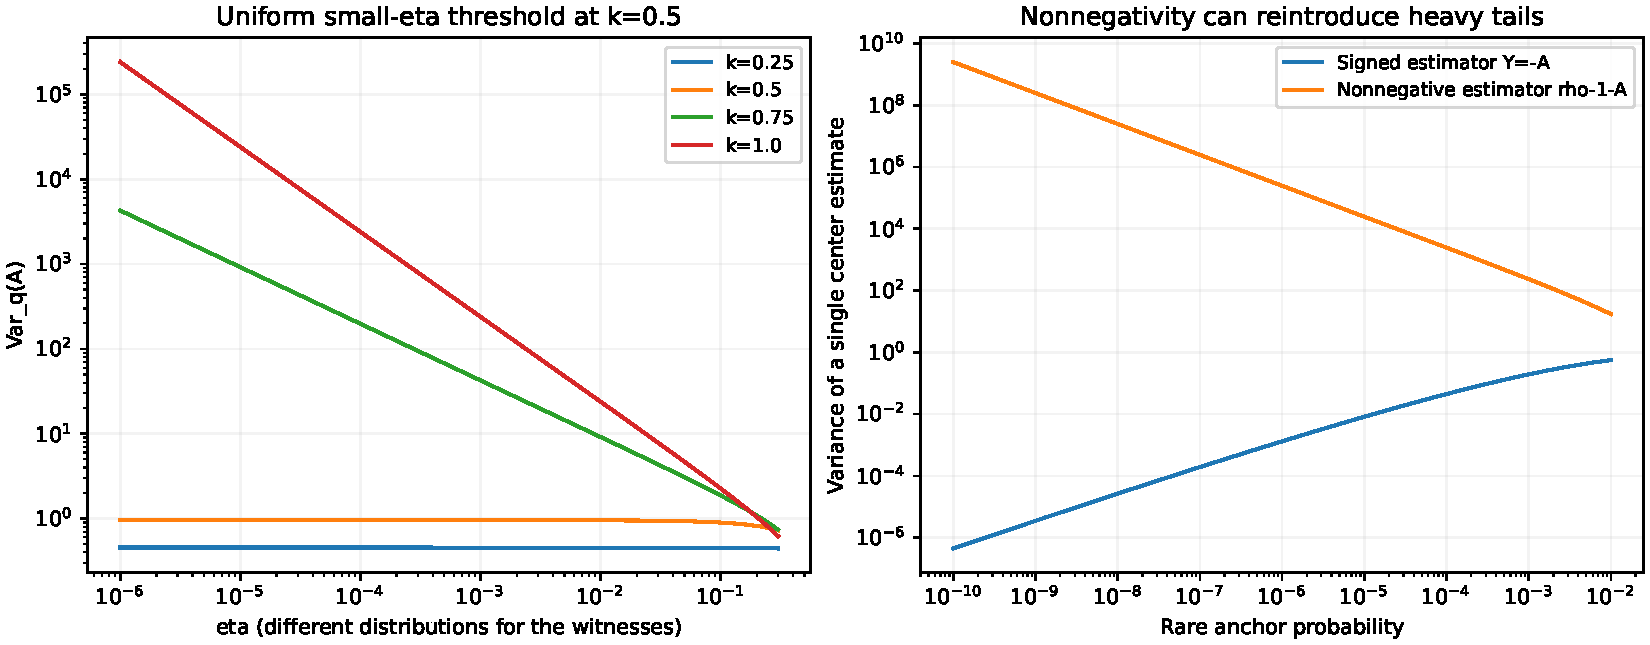
\includegraphics[width=\textwidth]{../../results/power-center-advantage/small-step-and-estimation.pdf}
 \caption{左：小步方差阈值的下界见证，不同形状使用不同分布族，不能当作同数据上的性能排名。右：逐样本非负中心估计可能重新引入概率比重尾。}
\end{figure}
\begin{figure}[htbp]
 \centering
 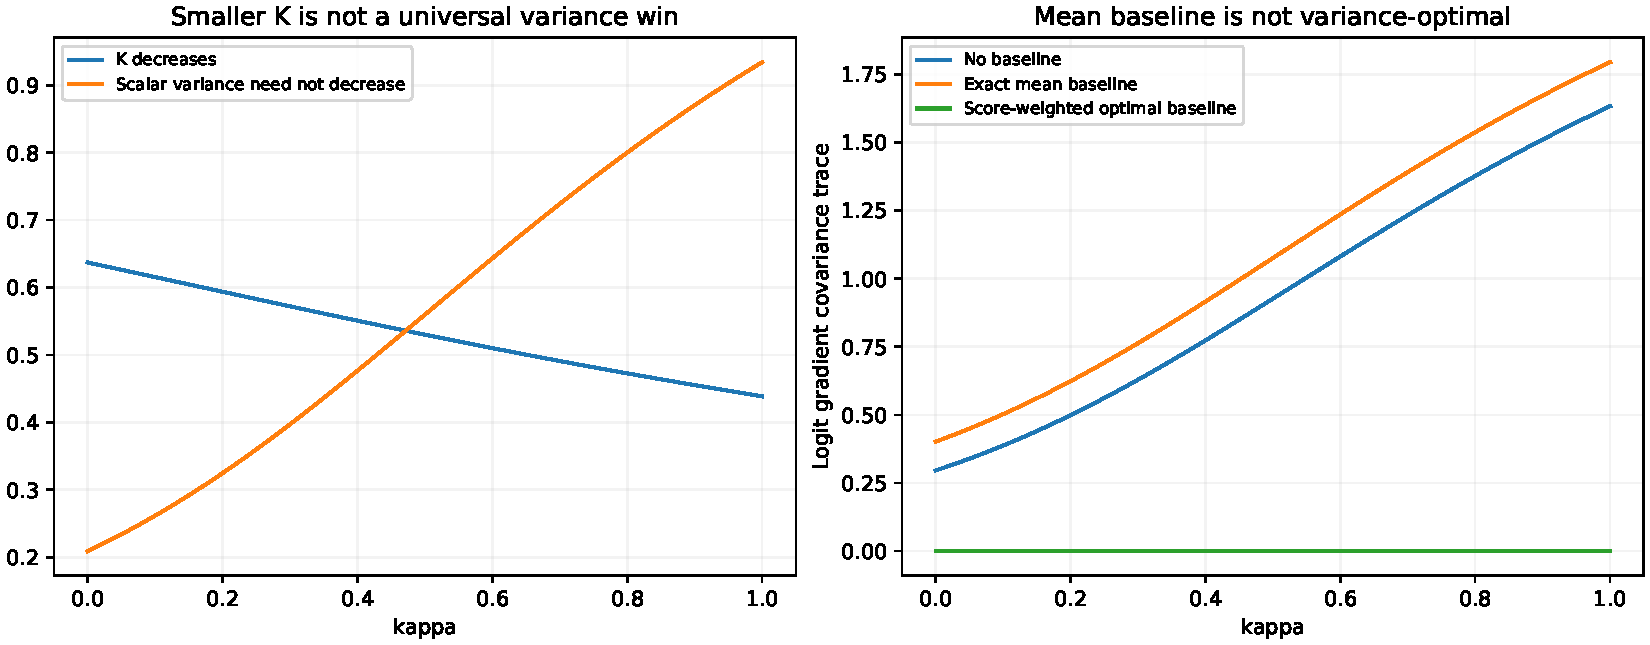
\includegraphics[width=\textwidth]{../../results/power-center-advantage/baseline-counterexample.pdf}
 \caption{同一二元输入下，$K$ 随形状下降但标量方差不必下降；均值 baseline 也不一定降低 logit 梯度方差。零方差最优 baseline 是二元例子的性质，不是一般网络结论。}
\end{figure}

数学核验与真实缓存审计见 \path{experiments/analysis/power_center_advantage.py}；真实缓存取原 64 条 t22 response 每条两个固定随机 reservoir 位置，共 128 个 prefix，对 20 组 $\kappa,\eta$ 精确求 action 条件矩。结果与所有实验统一维护在唯一实验报告；这些 CPU 模型分布统计不等于新 GPU 训练或全参数梯度方差。

\subsection{中心作为 MD 目标的散度代理}

\begin{theorem}[教师中心与精确 MD 目标的比较]
\label{thm:power-md-center-comparison}
对 $0\le\kappa\le1$、$0<\eta<1$，有逐点生成函数界和散度界
\begin{align}
 (1-\kappa)\omega_{\kappa,\eta}(x)
 &\le\phi_{\kappa,\eta}(x)\le\omega_{\kappa,\eta}(x),\\
 (1-\kappa)\mathcal J_{\kappa,\eta}(q;T)
 &\le K_{\kappa,\eta}(q,T)\le\mathcal J_{\kappa,\eta}(q;T).
 \label{eq:power-md-center-sandwich}
\end{align}
当 $\kappa<1$，$K$ 与 $\mathcal J$ 可互相控制；当 $\kappa=0$ 时相等。一般 $\kappa>0,\eta<1$ 下，$-A(T/p)$ 是 $\mathcal J$ 的梯度，却不是 $K(T,p)$ 的梯度。
\end{theorem}

\begin{proof}
记 $B=1-\eta+\eta x^\kappa$，两种生成函数的曲率比为
\begin{equation}
 \frac{\phi''(x)}{\omega''(x)}
 =1-\frac{\kappa(1-\eta)}B\in[1-\kappa,1].
\end{equation}
故 $\phi-(1-\kappa)\omega$ 与 $\omega-\phi$ 均为凸函数，在一处的函数值和导数为零，因而处处非负。对概率比求期望得到散度界。要计算中心作为当前分布函数的梯度，应用透视函数微分公式，得到
\begin{align}
 \frac\partial{\partial p_a}K_{\kappa,\eta}(p,T)
 &=\phi(x)-x\phi'(x)\\
 &=-A(x)+\frac{x^\kappa}{1-\eta+\eta x^\kappa}-1,
 \qquad x=T_a/p_a.
 \label{eq:power-md-center-gradient-difference}
\end{align}
额外项在 $\kappa>0,\eta<1$ 时通常随 action 改变，不能作为单纯形上的常数乘子消去。$\kappa=0$ 或 $\eta=1$ 时该项为零。
\end{proof}

这个比较给出一个可用的误差解释：若固定 $\kappa<1$ 且精确中心 $K\le\epsilon$，则 $\mathcal J\le\epsilon/(1-\kappa)$。它控制新的教师目标，不控制任意大的原 teacher reverse KL；当 $\kappa$ 接近一时该代理界退化。

两个目标的局部尺度也不同。记 $\delta=T/q-1$ 且全部比率一致趋一，则
\begin{align}
 \mathcal J_{\kappa,\eta}(q;T)
 &=\tfrac12\E_q\delta^2+O(\E_q|\delta|^3),\\
 K_{\kappa,\eta}(q,T)
 &=\tfrac12[1-\kappa(1-\eta)]\E_q\delta^2+O(\E_q|\delta|^3).
\end{align}
依据是 $\omega''(1)=1$ 与 $\phi''(1)=1-\kappa(1-\eta)$，一次项均因规范化消失。$D_\kappa$ 与 $\mathcal J_{\kappa,\eta}$ 的二阶局部 Fisher 尺度相同，$K$ 额外带有形状相关系数；三个数值不能直接作为同一训练误差混合比较。

\begin{figure}[H]
 \centering
 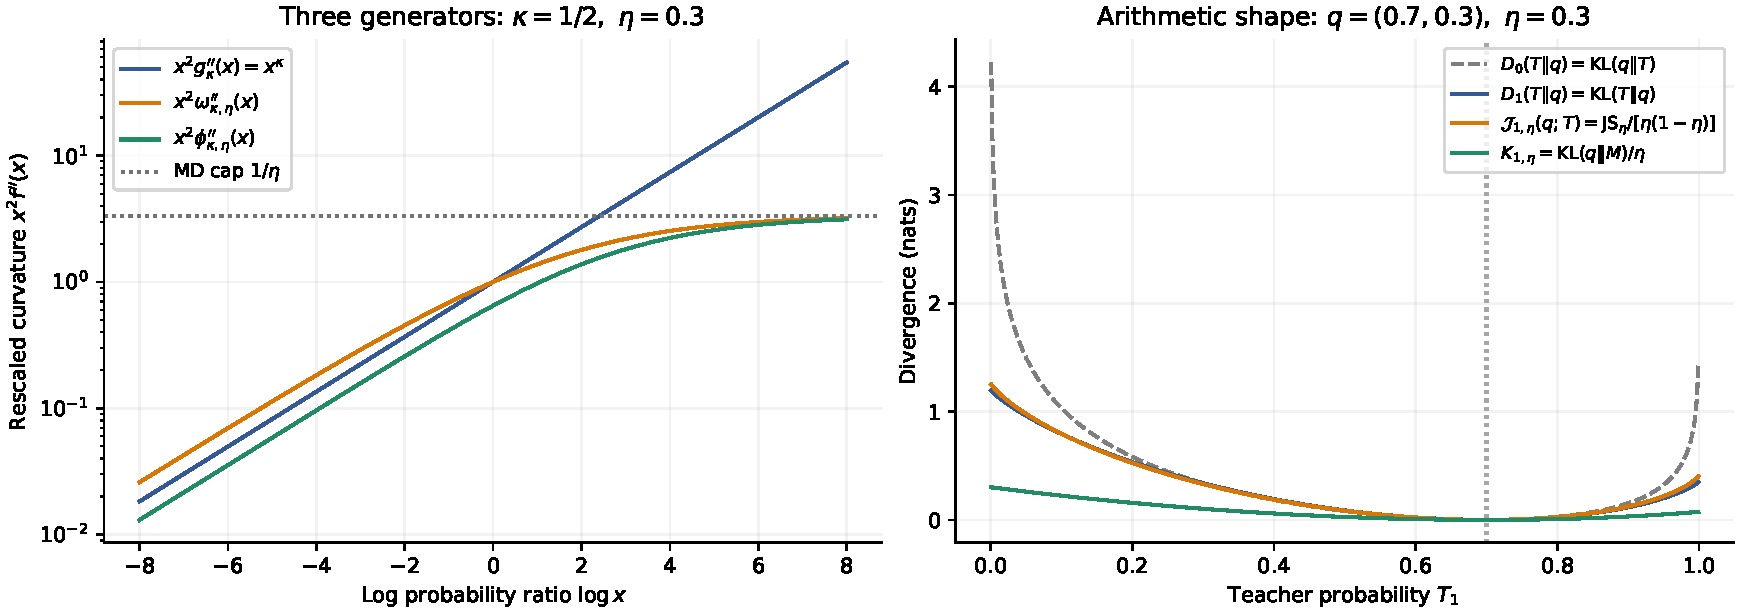
\includegraphics[width=\textwidth]{../../results/power-divergence-relations/families-and-curvature.pdf}
 \caption{三种散度的解析函数比较。左图在 $\kappa=1/2,\eta=0.3$ 时比较乘以 $x^2$ 的生成函数曲率；MD 曲率被 $1/\eta$ 统一控制，中心曲率更小。右图固定 $q=(0.7,0.3)$、$\eta=0.3$，让教师 $T=(T_1,1-T_1)$ 变化；算术形状的重心散度、精确 MD 目标和教师中心分别是 forward KL、归一化 JS 和对混合分布的 reverse KL。所有曲线直接计算公式，不来自训练或模型实验。}
 \label{fig:power-divergence-curvature}
\end{figure}

图的生成入口为 \path{experiments/plotting/plot_power_divergence_relations.py}；参数与公式范围保存在 \path{results/power-divergence-relations/figure.json}。

\begin{corollary}[精确外层的教师监督噪声可求和]
\label{cor:power-md-summable-variance}
固定 $0<\kappa\le1/2$、$0<\eta<1$，采用每步精确幂均值目标的外层 $q_{n+1}=m_{\kappa,\eta}(q_n,T)$。令
\begin{equation}
 V_n=\Var_{q_n}\!\left[A_{\kappa,\eta}(T/q_n)+K_{\kappa,\eta}(q_n,T)\right],
 \qquad C_0=\KL(T\Vert q_0).
\end{equation}
则对 $N\ge1$，
\begin{align}
 V_N&\le\frac{C_0}{\kappa(1-\kappa)(1-\eta)^2\eta N},\\
 \sum_{n=1}^N V_n&\le\frac{C_0}{\kappa(1-\kappa)(1-\eta)^2\eta}.
 \label{eq:power-md-summable-variance}
\end{align}
若各 outer 起点的 score 统一满足 $\|\psi_n(a)\|\le S$，则中心化 teacher score 单样本梯度的协方差 trace 也分别不超过右侧乘以 $S^2$。
\end{corollary}

\begin{proof}
第~\ref{thm:center-advantage-variance}~定理给出 $V_n\le K_n/[\kappa(1-\kappa)(1-\eta)^2]$；第~\ref{thm:power-md-center-comparison}~定理给出 $K_n\le\mathcal J(q_n;T)$。将两者与最后迭代界相乘，得到第一式。三点进展的望远镜求和给出 $\eta\sum_{n=1}^N\mathcal J(q_n;T)\le C_0$，代入得到第二式。梯度方差不超过其二阶矩，且 $\E_{q_n}\|\psi_n B_n\|^2\le S^2V_n$，得到带 score 的结论。
\end{proof}

可求和性针对同一固定 prefix、精确刷新分布和未标准化的教师监督。它并不比较每个输入上不同 $\kappa$ 的实际方差，也不覆盖任意神经网络 inner 残差或不断改变的 prefix 访问测度。该推论把“鲁棒散度有界”“新目标的精确 MD 下降”和“误差相关方差界”连接为一条完整论证；无需先做大模型扫描来确定这些条件性质。


\section{平方根形状与最优性的判据}
\label{sec:power-half-and-optimality}
\subsection{平方根形状的有界自然梯度与显式动力学}

由式~\eqref{eq:proximal-natural-velocity}，$\|v_\kappa\|_F^2=\Var_q(\rho^\kappa)/\kappa^2$。当 $0<\kappa\le1/2$，$2\kappa\le1$，Jensen 不等式给出 $\E_q\rho^{2\kappa}\le(\E_q\rho)^{2\kappa}=1$，于是
\begin{equation}
 \|v_\kappa\|_F^2\le\frac{1-a_\kappa^2}{\kappa^2}\le\frac1{\kappa^2}.
 \label{eq:proximal-natural-speed-bound}
\end{equation}
该界对任意完整支持的 $q,T$ 成立，不需要给 teacher 或 student 指定统一概率下界。对于 $\kappa>1/2$，取 $q=(\varepsilon,1-\varepsilon)$、$T=(c,1-c)$，$0<c<1$ 固定，则
\begin{equation}
 \Var_q(\rho^\kappa)
 =\varepsilon(1-\varepsilon)
 \left[(c/\varepsilon)^\kappa-((1-c)/(1-\varepsilon))^\kappa\right]^2
 \sim c^{2\kappa}\varepsilon^{1-2\kappa}\longrightarrow\infty.
\end{equation}
几何端点 $\kappa=0$ 也没有统一界：固定 $q=(1/4,3/4)$、令 $T=(\varepsilon,1-\varepsilon)$，$\Var_q\log(T/q)$ 随 $\varepsilon\to0$ 发散。故 $0<\kappa\le1/2$ 是这个自然梯度族具有统一 Fisher 速度界的区间。确定性的 Fisher 速度与随机参数梯度方差是不同对象，不能把这个结论直接写成完整训练梯度的方差定理。

在平方根点 $\kappa=1/2$，$a=\sum\sqrt{qT}$，并有 $\E_q\rho=1$，因此
\begin{equation}
 \|v_{1/2}\|_F^2=4(1-a^2)\le4,\qquad
 D_{1/2}(T\Vert q)=4(1-a).
\end{equation}
由 Lyapunov 等式，连续流满足
\begin{equation}
 \frac{da}{dt}=1-a^2,
 \qquad a(t)=\tanh(t+\operatorname{artanh}a(0)),\quad q\ne T.
 \label{eq:proximal-hellinger-flow}
\end{equation}
证明是 $dD_{1/2}/dt=-4\,da/dt=-4(1-a^2)$，然后积分 $da/(1-a^2)=dt$。$q=T$ 时 $a=1$ 且流恒定。进一步，$D'=-(1+a)D$，由于 $0<a\le1$，有
\begin{equation}
 D(0)e^{-2t}\le D(t)\le D(0)e^{-t}.
\end{equation}
若写 $a=\cos\vartheta$，则 $d\vartheta/dt=-\sin\vartheta$。平方根形状既有球面解释，也有显式 teacher 接近度和有界 Fisher 速度。这使它成为一个有数学依据的候选点，尚不能据此断言其训练性能优于其他形状。

\begin{figure}[htbp]
 \centering
 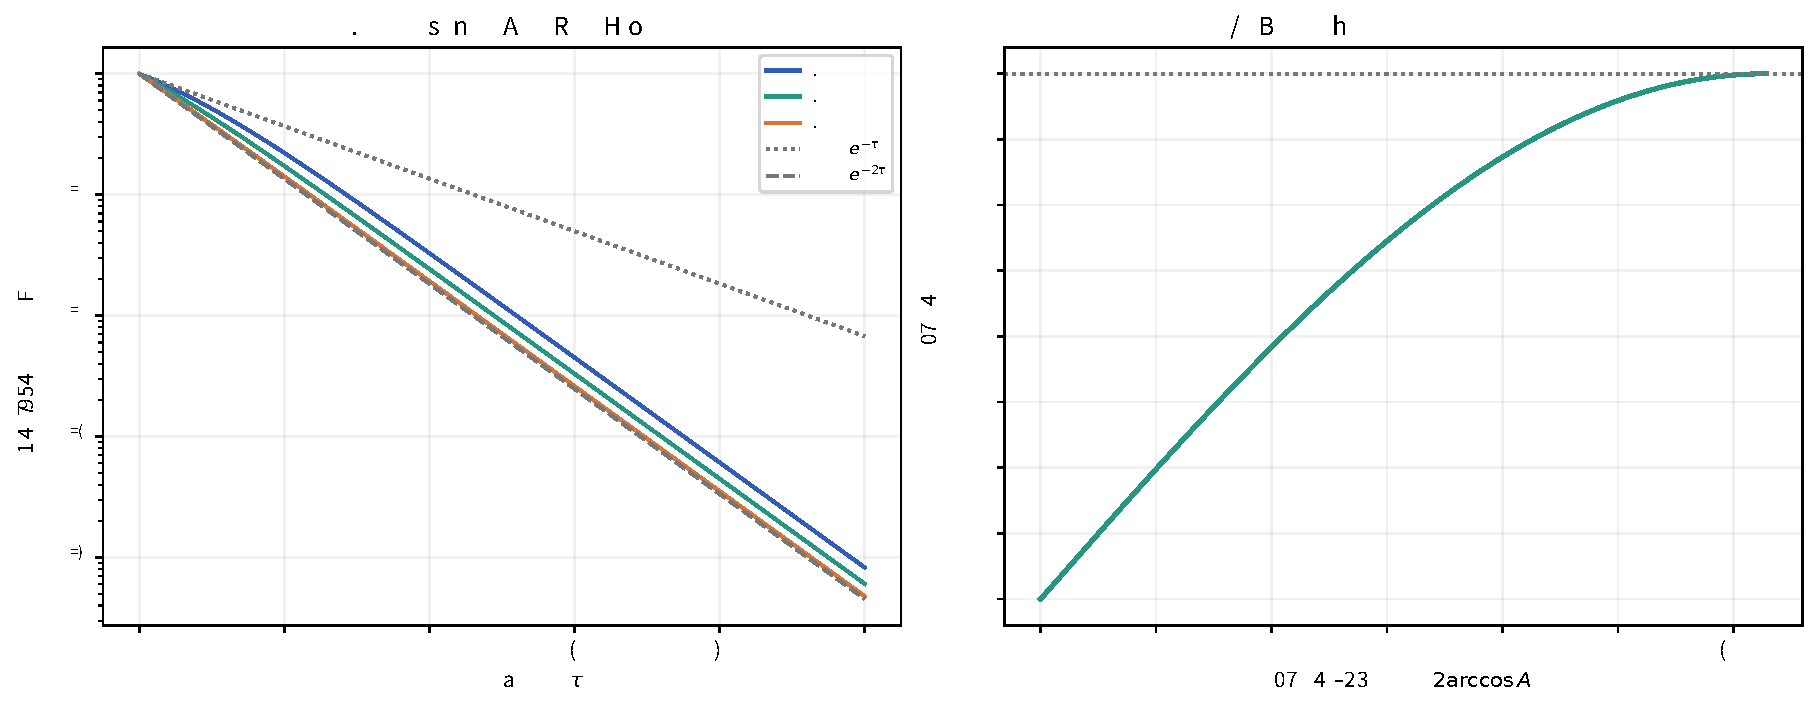
\includegraphics[width=\textwidth]{../../results/proximal-family-geometry/hellinger-flow.pdf}
 \caption{平方根形状的连续动力学。左图由 $a(t)=\tanh(t+\operatorname{artanh}a(0))$ 精确生成，归一化散度位于两个指数包络之间；右图将 Fisher 速度写成到 teacher 的 Fisher--Rao 距离函数，展示统一上界 2。}
\end{figure}

\subsection{共同目标下的局部最优形状}

令 $r=\log(T/q)$，$w_\kappa=(\rho^\kappa-\E_q\rho^\kappa)/\kappa$，$w_0=C_qr$，于是 $v_\kappa=qw_\kappa$。对固定 Fisher 速度的单位方向 $u_\kappa=v_\kappa/\|v_\kappa\|_F$，reverse KL 的一阶下降量为
\begin{equation}
 -\nabla\KL(q\Vert T)^\top u_\kappa
 =\frac{\E_q[rw_\kappa]}{\sqrt{\E_qw_\kappa^2}}
 \le\sqrt{\Var_qr}.
\end{equation}
这是 Cauchy--Schwarz 不等式，几何形状 $\kappa=0$ 取得等号。对 forward KL，同样有
\begin{equation}
 -\nabla\KL(T\Vert q)^\top u_\kappa
 =\frac{\E_q[\rho w_\kappa]}{\sqrt{\E_qw_\kappa^2}}
 \le\sqrt{\Var_q\rho},
\end{equation}
算术形状 $\kappa=1$ 取得等号。更一般地，$\kappa$ 自己对应的散度具有自己的自然梯度最陡方向。这个局部确定性最优性与平方根形状的最坏矩性质是不同标准，不能由有界方差推出对任何共同评价目标的最优收敛速度。
\subsection{目标自然速度的锐上界与另一个极小极大形状}

对 $0<\kappa<1/2$，令 $X=\rho^\kappa$、$r=1/\kappa>2$，则 $\E_qX^r=1$。写成 $X^2=X^{(r-2)/(r-1)}(X^r)^{1/(r-1)}$，对两因子使用共轭指数 $(r-1)/(r-2)$ 与 $r-1$ 的 Hölder 不等式，得到
\begin{equation}
 \E_qX^2\le(\E_qX)^{(r-2)/(r-1)}
 =(\E_qX)^{(1-2\kappa)/(1-\kappa)}.
\end{equation}
令 $a=\E_qX\in[0,1]$，$\gamma=(1-2\kappa)/(1-\kappa)$。于是 $\Var_qX\le a^\gamma-a^2$。驻点满足 $a^{2-\gamma}=\gamma/2$，代回并记 $b=(1-2\kappa)/[2(1-\kappa)]$，得到锐上界
\begin{equation}
 \boxed{\sup_{q,T}\|v_\kappa\|_F^2
 =C_{\mathrm{vel}}(\kappa)
 =\frac{b^{1-2\kappa}(1-b)}{\kappa^2}}.
\end{equation}
锐性由 $q=(b,1-b)$、$T\to(1,0)$ 达到：$X$ 仅取 $b^{-\kappa}$ 与零，插值不等式和驻点条件同时成立。完整支持分布以极限逼近这个值。$\kappa=1/2$ 的上确界为 4；$\kappa=0$ 或 $\kappa>1/2$ 无有限上界。

在优化 $b$ 后使用包络导数，$d\log C_{\mathrm{vel}}/d\kappa=-2/\kappa-2\log b$。唯一最小点满足
\begin{equation}
 \log\frac{1-2\kappa_\star}{2(1-\kappa_\star)}=-\frac1{\kappa_\star}.
\end{equation}
左侧加 $1/\kappa$ 的导数为 $-1/[(1-2\kappa)(1-\kappa)]-1/\kappa^2<0$，在零点附近趋于正无穷，在 $1/2$ 附近趋于负无穷，故根唯一。根和常数由第一方参考函数 \texttt{minimax\_velocity\_shape}、\texttt{worst\_fisher\_speed\_squared} 计算并验证。

这个最优形状针对 target 的最坏 Fisher 速度上界及小步标量监督方差，与其他拟合散度的误差相关噪声常数最优 $\kappa_{\mathrm{fit}}=1/2$ 是不同标准。更小的最大速度不自动代表更快学习；部分 teacher 方向也可能变慢。平方根的闭式性质和这个极小极大准则都不能替代任务指标。

\begin{figure}[htbp]
 \centering
 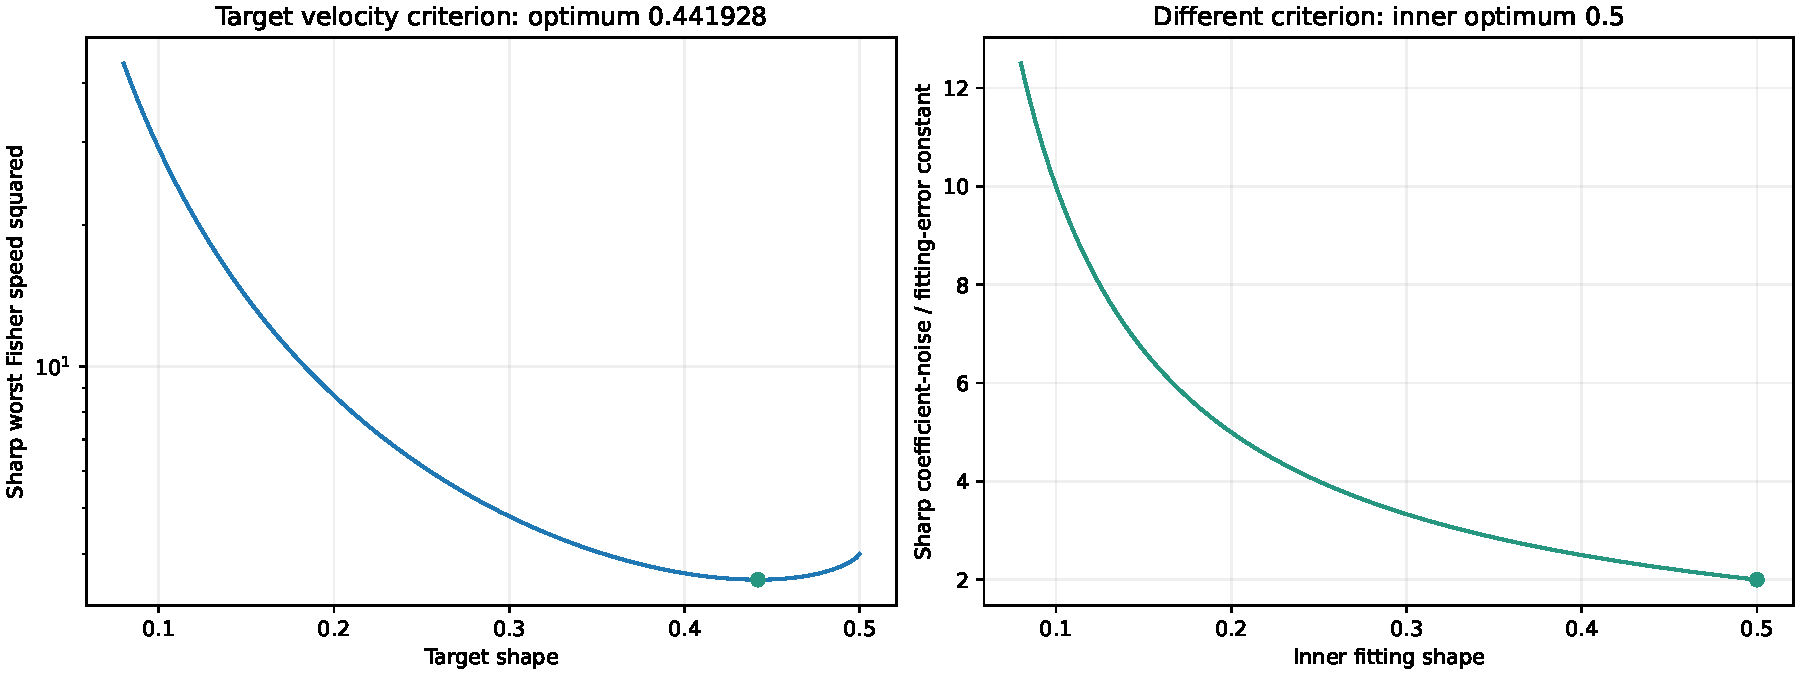
\includegraphics[width=\textwidth]{../../results/power-mean-20261013/two-minimax-criteria.pdf}
 \caption{两个不同的极小极大标准。左图是 target 速度的锐上界，最小点为 $0.441928$；右图是第~\ref{sec:power-projection}~节其他拟合目标的噪声与损失锐相对常数 $1/\kappa_{\mathrm{fit}}$，最小点为 $1/2$。二者都不直接等于最高任务准确率。}
\end{figure}

\subsection{教师误差归一化的锐噪声常数}

\begin{theorem}[平方根形状的相对误差噪声最优性]
\label{thm:power-relative-noise-optimum}
固定 $0<\kappa\le1/2$。令 $\rho=T/q$，小步教师监督为 $A_\kappa^0=(\rho^\kappa-1)/\kappa$，中心为 $K_\kappa^0=[1-\E_q\rho^\kappa]/\kappa$。对至少二元、严格正且 $q\ne T$ 的分布取上确界，有
\begin{align}
 \sup_{q,T}\frac{\Var_qA_\kappa^0}{D_\kappa(T\Vert q)}&=\frac1\kappa,\\
 \sup_{q,T}\frac{\Var_qA_\kappa^0}{K_\kappa^0}&=\frac1{\kappa(1-\kappa)}.
 \label{eq:power-relative-noise-sharp}
\end{align}
在 $\kappa\in[0,1]$ 的幂散度族内，两个准则都由 $\kappa=1/2$ 唯一最小化，锐常数分别为 2 和 4。端点零与 $\kappa>1/2$ 没有有限的统一相对误差常数。
\end{theorem}

\begin{proof}
第~\ref{thm:center-advantage-variance}~定理证明了 $\Var_q(\rho^\kappa)\le[1-a_\kappa]/(1-\kappa)$。除以 $\kappa^2$，再使用 $D_\kappa=[1-a_\kappa]/[\kappa(1-\kappa)]$ 与 $K_\kappa^0=[1-a_\kappa]/\kappa$，得到两个上界。

取 $q=(v,1-v)$、$T=(v^2,1-v^2)$，$v\to0$，则 $\rho=(v,1+v)$。对固定 $0<\kappa\le1/2$，
\begin{equation}
 a_\kappa=v^{1+\kappa}+(1-v)(1+v)^\kappa
 =1-(1-\kappa)v+o(v).
\end{equation}
同理 $a_{2\kappa}=1-(1-2\kappa)v+o(v)$，于是
\begin{equation}
 \Var_qA_\kappa^0=v/\kappa^2+o(v),\quad
 D_\kappa=v/\kappa+o(v),\quad
 K_\kappa^0=(1-\kappa)v/\kappa+o(v).
\end{equation}
相除逼近两个上界，证明锐性。两个常数在 $(0,1/2]$ 上严格递减，最小值均在 $1/2$。

若 $1/2<\kappa<1$，取 $q=(v,1-v)$、$T=(1/2,1/2)$，监督方差按 $v^{1-2\kappa}$ 发散，而 $D_\kappa$ 和 $K_\kappa^0$ 有统一上界。$\kappa=1$ 时方差按 $1/v$ 增长，forward KL 只按 $\log(1/v)$ 增长，且 $K_1^0=0$。$\kappa=0$ 时固定非对称正 $q$，使一个教师概率趋零，方差按平方 log 增长，reverse KL 只按一次 log 增长。故其余形状不存在有限统一常数。
\end{proof}

这个最优性比较的是误差相关噪声常数，并非绝对噪声常数 $C_{\mathrm{vel}}$。所有 $D_\kappa$ 已采用同一局部 Fisher 规范化；其全局值仍随 $\kappa$ 改变。平方根使噪声相对于自身教师误差的最坏放大最小，不意味着每个输入上的方差或任务正确率都最优。

\subsection{平方根中间分布的有限步 Hellinger 进展}

平方根 target 把冻结学生与教师的平方根概率加权后归一化，而不是直接对概率作算术平均。记 $u=\sqrt q$、$v=\sqrt T$、$a=u^\top v$、$w=1-\eta$，则
\begin{equation}
 \sqrt{m_{1/2,\eta}}=\frac{wu+\eta v}{\sqrt Z},\qquad
 Z=w^2+\eta^2+2w\eta a.
 \label{eq:power-half-normalized-chord}
\end{equation}
$u,v$ 在正单位球面上。归一化的正线性组合位于两者张成的二维平面及短圆弧上，因而是 Fisher--Rao 路径的一个参数化；$\eta$ 通常不是弧长比例。对 $q=T$，该路径恒定。

\begin{theorem}[平方根 target 的精确亲和度与收缩]
\label{thm:power-half-discrete-contraction}
采用不带 $1/2$ 因子的 $H^2(q,T)=\sum_a(\sqrt{q_a}-\sqrt{T_a})^2=2(1-a)$。精确平方根更新满足
\begin{align}
 a^+&=\sum_a\sqrt{m_aT_a}=\frac{wa+\eta}{\sqrt Z},\\
 H^2(m,T)&\le(1-\eta)H^2(q,T).
 \label{eq:power-half-discrete-progress}
\end{align}
因此固定教师下反复精确更新得到 $H^2(q_N,T)\le(1-\eta)^NH^2(q_0,T)$。目标与锚点的平方根夹角 $\vartheta_{qm}$ 还满足
\begin{equation}
 \cos\vartheta_{qm}=\frac{w+\eta a}{\sqrt Z},\qquad
 \sin^2\vartheta_{qm}=\frac{\eta^2(1-a^2)}Z.
\end{equation}
这些都是精确分布更新的性质，不要求对 teacher 概率指定统一下界。
\end{theorem}

\begin{proof}
式~\eqref{eq:power-half-normalized-chord} 与 $v$ 内积直接给出 $a^+$。由于 $a\le1$，$Z\le(w+\eta)^2=1$，且 $wa+\eta>0$，有 $a^+\ge wa+\eta$。所以 $1-a^+\le w(1-a)$，乘以二即得 Hellinger 收缩。每轮重复应用即可得 $N$ 步界。与 $u$ 内积得到第二个夹角的余弦；再计算 $Z-(w+\eta a)^2=\eta^2(1-a^2)$，得到正弦平方。
\end{proof}

几何端点在同一 Hellinger 指标下没有严格小于一的分布无关单步收缩因子。固定 $0<\eta<1$，取 $q_\epsilon=(\epsilon,1-\epsilon)$、$T=(1/2,1/2)$，则几何 target 的第一坐标为
\begin{equation}
 m_{0,\eta,1}
 =\frac{\epsilon^{1-\eta}}{\epsilon^{1-\eta}+(1-\epsilon)^{1-\eta}}
 \longrightarrow0.
\end{equation}
因此 $q_\epsilon$ 与其几何 target 都趋于 $(0,1)$，两者到 $T$ 的 $H^2$ 都趋于 $2(1-1/\sqrt2)>0$，收缩比趋于一。平方根点的 $(1-\eta)$ 因子加强了相对于几何端点的统一全局 Hellinger 保证；教师附近的局部因子仍与其他形状相同，见后一定理。

\begin{corollary}[平方根精确外层的几何噪声界]
\label{cor:power-half-geometric-noise}
固定教师和 $0<\eta<1$，反复执行精确平方根 target。令 $V_n=\Var_{q_n}A_{1/2,\eta}(T/q_n)$，则
\begin{align}
 V_n&\le\frac{4H^2(q_n,T)}{(1-\eta)^2}
 \le\frac{4(1-\eta)^nH^2(q_0,T)}{(1-\eta)^2},\\
 \sum_{n=0}^\infty V_n&\le\frac{4H^2(q_0,T)}{\eta(1-\eta)^2}
 \le\frac8{\eta(1-\eta)^2}.
\end{align}
若 score 范数统一不超过 $S$，中心化教师梯度的协方差 trace 满足相应右侧乘以 $S^2$ 的界。
\end{corollary}

\begin{proof}
第~\ref{thm:center-advantage-variance}~定理给出 $V_n\le D_{1/2}(T\Vert q_n)/[(1/2)(1-\eta)^2]$。用 $D_{1/2}=2H^2$ 与前一定理的 Hellinger 收缩得到第一式。对 $n\ge0$ 求和，几何级数为 $1/\eta$；最后使用 $H^2\le2$。梯度二阶矩由 score 范数界控制。
\end{proof}

这比一般 MD 的 $O(1/N)$ 监督方差界更明确：平方根精确外层具有同一有界误差量驱动的几何噪声上界，累计上界不依赖可能任意大的初始 KL。它仍要求固定前缀和精确 target 更新；实际 BPO 误差会另外进入进展界。

\begin{figure}[H]
 \centering
 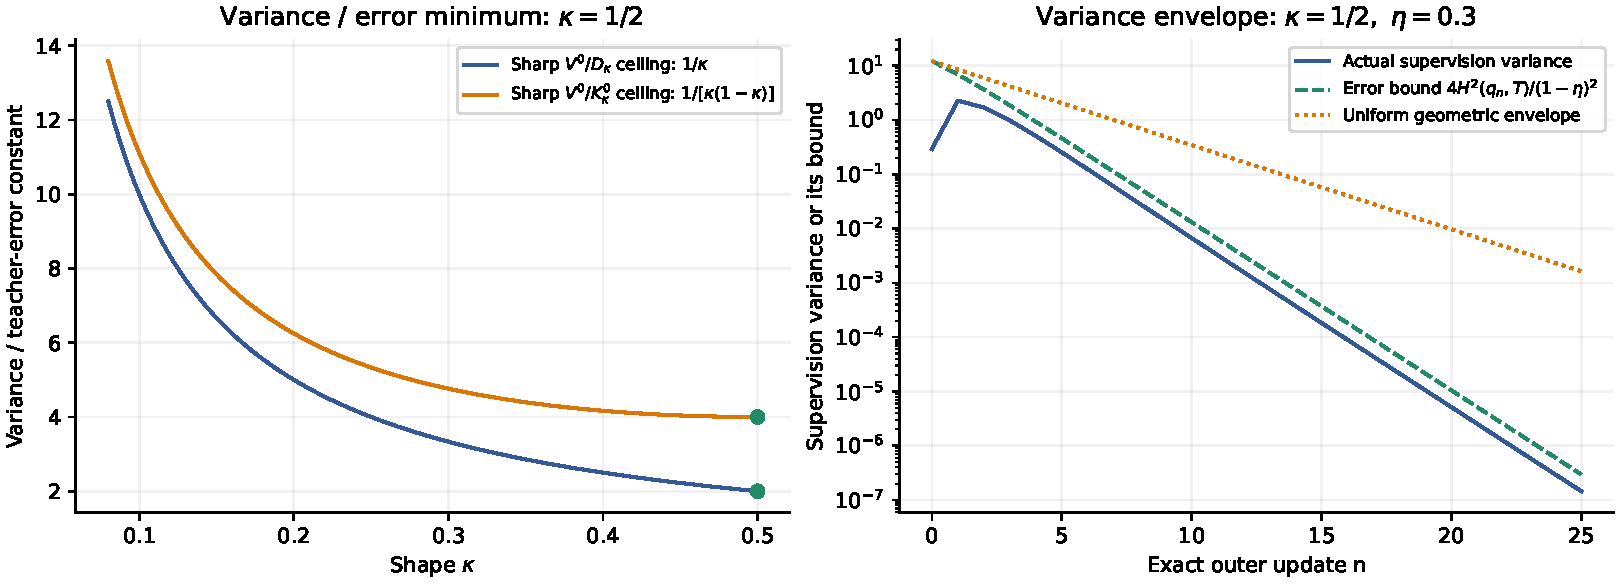
\includegraphics[width=\textwidth]{../../results/chapter9-restructure/relative-noise-and-convergence.pdf}
 \caption{左图以相对教师误差的锐噪声常数选择形状，两个准则均在 $\kappa=1/2$ 最小。右图对 $q_0=(0.999,0.001)$、$T=(0.05,0.95)$、$\eta=0.3$ 做精确平方根迭代。Hellinger 驱动的方差上界和统一几何包络下降，实际标量方差在第一步却增大。几何包络控制收敛过程，并不保证实际方差逐步单调。}
 \label{fig:power-relative-noise-convergence}
\end{figure}

\subsection{所有形状共享局部收敛率}

\begin{theorem}[幂均值的局部展开与共同收缩因子]
\label{thm:power-common-local-rate}
固定正支持教师 $T$、$0<\eta<1$、$0\le\kappa\le1$。令 $q=T+\epsilon h$，其中 $\sum h_a=0$、$h\ne0$，并使全部 $\epsilon h_a/T_a$ 一致趋零。记 $w=1-\eta$、$S_h=\sum_ah_a^2/T_a$，则
\begin{equation}
 m_a=T_a+w\epsilon h_a
 +\frac{(\kappa-1)w\eta}{2}\epsilon^2
       \left(\frac{h_a^2}{T_a}-T_aS_h\right)+O(\epsilon^3).
 \label{eq:power-second-order-target}
\end{equation}
若凸生成函数 $g$ 在一附近三阶可微且 $g''(1)>0$，则
\begin{equation}
 \frac{D_g(m\Vert T)}{D_g(q\Vert T)}
 =(1-\eta)^2+O(\epsilon).
 \label{eq:power-local-divergence-rate}
\end{equation}
因此在同一局部评价散度下，平方根形状没有优于其他形状的一阶概率误差收缩率。固定 $q,\eta$ 的 BPO logits Hessian 同样不因 $\kappa$ 改善。
\end{theorem}

\begin{proof}
对 $\kappa>0$，先展开
\begin{equation}
 (1-\eta)q_a^\kappa+\eta T_a^\kappa
 =T_a^\kappa\left[1+w\kappa\epsilon\frac{h_a}{T_a}
 +\frac{w\kappa(\kappa-1)}2\epsilon^2\frac{h_a^2}{T_a^2}
 +O(\epsilon^3)\right].
\end{equation}
再使用 $(1+x)^{1/\kappa}$ 的二阶展开，未归一化幂均值为
\begin{equation}
 \widetilde m_a=T_a+w\epsilon h_a
 +\frac{(\kappa-1)w\eta}{2}\epsilon^2\frac{h_a^2}{T_a}+O(\epsilon^3).
\end{equation}
求和时一次项消失，得到 $Z=1+[(\kappa-1)w\eta/2]\epsilon^2S_h+O(\epsilon^3)$。除以 $Z$ 即得第一式。几何端点可以直接展开 $q_a^wT_a^\eta$，得到同一式子中 $\kappa=0$ 的结果。

将 $g$ 加上线性项使 $g'(1)=0$ 不改变散度。Taylor 展开给出 $D_g(q\Vert T)=g''(1)\epsilon^2S_h/2+O(\epsilon^3)$。用 $m-T=w\epsilon h+O(\epsilon^2)$ 再展开，得到 $D_g(m\Vert T)=g''(1)w^2\epsilon^2S_h/2+O(\epsilon^3)$。$g''(1)S_h>0$，相除得到第二式。BPO 的曲率结论由第~\ref{sec:power-bpo-algorithm}~节的精确二次型给出。
\end{proof}

\subsection{形状选择取决于明确的评价标准}

\begin{center}
\small
\begin{tabular}{p{55mm}p{35mm}p{54mm}}
\toprule
评价标准 & 结论 & 条件与含义\\
\midrule
小步监督的分布无关有限方差 & $0<\kappa\le1/2$ & $1/2$ 是该区间的最大形状\\
小步方差相对教师误差的最坏比值 & $\kappa=1/2$ & $V\le2D_{1/2}=4H^2$，常数最优\\
最坏小步标量方差／Fisher 速度 & $\kappa_\star\simeq0.441928$ & 锐值 $3.527275$；平方根为 4\\
相同 Fisher 速度下的 reverse KL 局部下降 & $\kappa=0$ & 最陡确定性方向；无统一尾部界\\
相同 Fisher 速度下的 forward KL 局部下降 & $\kappa=1$ & 最陡确定性方向；小步最坏方差发散\\
当前学生采样的幂散度拟合噪声常数 & $\kappa_{\mathrm{fit}}=1/2$ & 拟合形状的最优性，不是 BPO target 最优性\\
固定 $q,\eta$ 的 BPO 条件数 & 对所有 $\kappa$ 相同 & 形状只改变 target 与初始残差\\
数学任务正确率与 NN 优化效率 & 尚无普遍最优点 & 不能用上述单一常数替代任务指标\\
\bottomrule
\end{tabular}
\end{center}

平方根点具有一个简洁的组合：球面中间 target、统一小步方差界、Hellinger 误差相关噪声和显式精确外层收缩。$\kappa_\star$ 则针对另一个明确准则将最坏小步标量方差上界从 4 降到约 3.5273。较小的方差常数同时可能缩小某些方向的信号；它不等于更高的梯度信噪比或更快的任务学习。

这些比较保持了同一个局部监督尺度：对所有形状，$A'_{\kappa,\eta}(1)=1$，等价于 $\partial_r f_{\kappa,\eta}(0)=\eta$。教师目标的生成函数也均满足 $\omega''_{\kappa,\eta}(1)=1$。形状改变的是远离教师时的路径和尾部响应；其小步方差差异没有通过一个额外的整体信号缩放制造。

有限步的共同 teacher 误差也没有统一的形状排序。固定 $\eta=0.3$，取 $q=(0.9,0.1)$、$T=(0.01,0.99)$，几何 target 的 Hellinger 误差低于平方根 target；改为 $q=(0.99,0.01)$、$T=(0.5,0.5)$，平方根 target 的 Hellinger 误差低于几何 target。两对输入都严格为正，直接代入闭式 target 即可验证。

\begin{figure}[H]
 \centering
 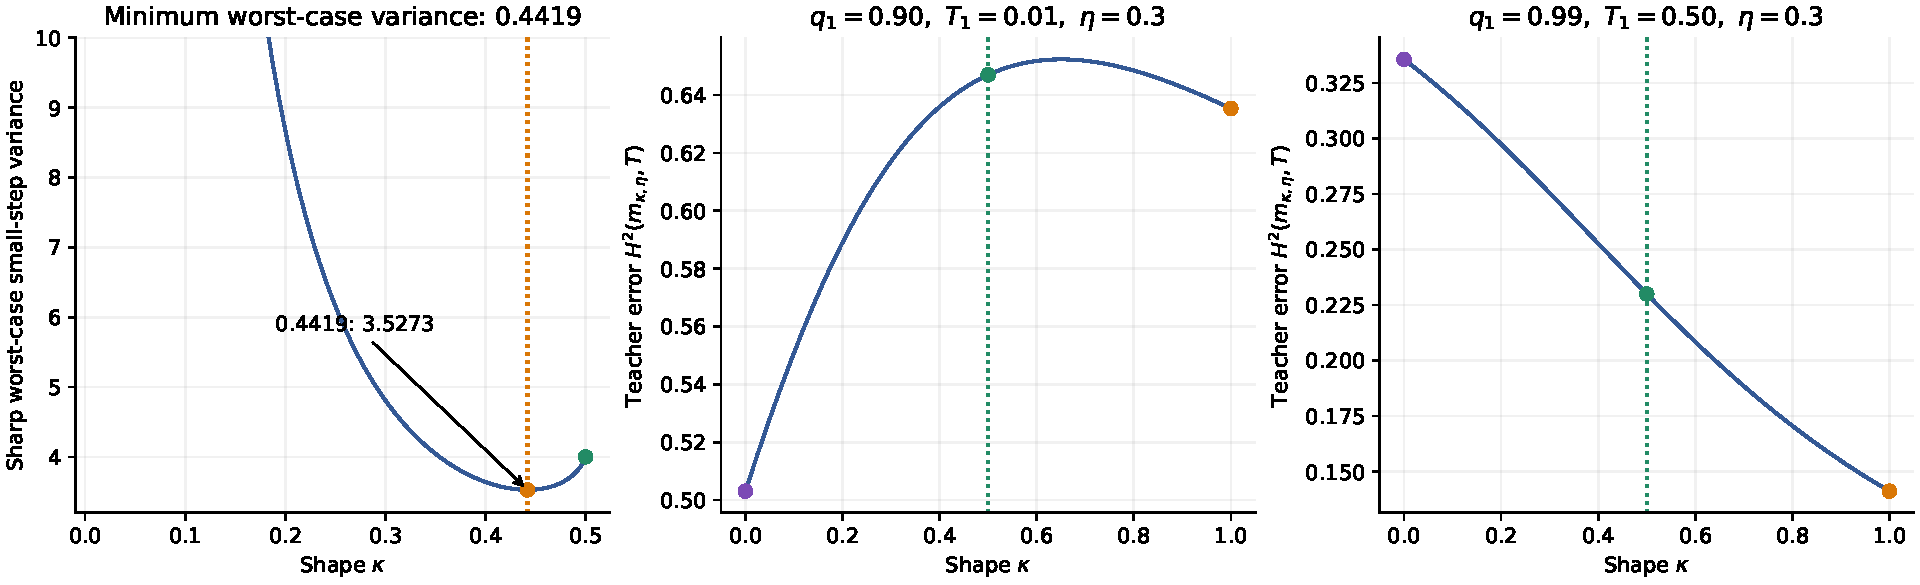
\includegraphics[width=\textwidth]{../../results/chapter9-restructure/kappa-criteria.pdf}
 \caption{形状的优势取决于评价标准。左图为锐最坏小步方差常数，最小点约为 $0.4419$，平方根点为 4。中、右图对同一 $\eta=0.3$ 使用两对固定二元分布，比较精确 target 后的同一 Hellinger 误差；曲线没有一致的形状排名。图只计算解析概率公式，不使用模型训练。}
 \label{fig:power-kappa-criteria}
\end{figure}

学生和教师的加权分布还可以用作辅助 action 提案，例如 $\mu_\zeta=(1-\zeta)q+\zeta T$。这与平方根监督 target 是两个选择：前者通过重要性校正估计原 $q$ 加权 BPO 损失，后者改变要拟合的目标。提案混合能控制重要性比率并在一些稀有 action 输入上改善相对方差，但没有每个输入都降低方差的保证。第~\ref{sec:power-estimators}~节给出无偏性、反例和排除重复 action 后的协方差半正定改进。


\section{中心估计与单轨迹的 action 估计}
\label{sec:power-estimators}
\label{sec:center-extensions}
\subsection{精确求和、Monte Carlo 与非负估计的代价}

若 teacher forward 能提供该前缀完整 logits，则使用完整 $q$ 权重直接求式~\eqref{eq:center-expanded-k}，不需要生成第二条 response。信号在 log 空间用 logaddexp 计算，避免先形成极大的 $T/q$。该中心可以按 prefix 缓存并冻结。

若采用独立 $a_i\sim q(\cdot\mid s)$，有无偏估计
\begin{equation}
 \widehat K=-\frac1M\sum_{i=1}^MA(a_i),\qquad
 \Var\widehat K=V/M.
\end{equation}
$\widehat K$ 单次可以为负；这不违背其非负期望。另一个逐样本非负无偏估计为
\begin{equation}
 \widehat K_+=\frac1M\sum_i[\rho(a_i)-1-A(a_i)].
\end{equation}
两者期望相同，方差一般不同。 它们在局部与最坏尾部上具有不同表现。若 $\rho=1+\epsilon h$、$\E_qh=0$ 且 $h$ 有界，令 $c_0=1-\kappa(1-\eta)$，则
\begin{align}
 -A&=-\epsilon h+\tfrac12c_0\epsilon^2h^2+O(\epsilon^3),\\
 \phi(\rho)&=\tfrac12c_0\epsilon^2h^2+O(\epsilon^3),\\
 \Var(-A)&=\epsilon^2\E_qh^2+O(\epsilon^3),\\
 \Var\phi(\rho)&=\tfrac14c_0^2\epsilon^4\Var_q(h^2)+O(\epsilon^5).
\end{align}
因此包括 $\kappa=0$ 在内，接近同分布时非负控制变量估计可把方差从二阶降至四阶；这需要概率比一致接近一，不能扩展到任意重尾输入。

取 $q=(\epsilon,1-\epsilon)$、$T=(1/2,1/2)$、固定 $\kappa>0,\eta<1$，原始估计方差按 $O(\epsilon\log^2(1/\epsilon))\to0$；非负估计的稀有项为 $\rho\sim1/(2\epsilon)$，其方差按 $1/(4\epsilon)$ 发散。这个 $\rho-1$ 控制变量保证非负性，却不能提供统一低方差保证。固定数据上也可能降低方差，应记录真实条件矩后判断。 即便原 KL 很小，也不能自动使用局部结论：取 $q=(\epsilon,1-\epsilon)$、$T=(\epsilon^{1/4},1-\epsilon^{1/4})$，有 $\KL(q\Vert T)\sim\epsilon^{1/4}\to0$，但非负估计的方差按 $\epsilon^{-1/2}$ 发散。概率比一致接近一比 KL 小更强。

如果独立中心估计与当前 action 独立，$\Var[A(a)+\widehat K]=V+V/M$。估计中心不会自动降低标量 advantage 方差。若中心与 advantage 使用同一组 $M$ 个 action，固定参数下
\begin{equation}
 \E\left[\frac1M\sum_i(A_i-\bar A)\psi_i\right]
 =\frac{M-1}{M}\operatorname{Cov}_q(A,\psi).
\end{equation}
这个恒等式由展开双重和得到：$M$ 个同索引项贡献 $\E A\psi$，$M(M-1)$ 个异索引项贡献 $\E A\E\psi$。$M=1$ 时更新为零。 若同一个 action 改用非负估计 $\widehat K_+=\rho-1-A$，则
\begin{equation}
 A(a)+\widehat K_+(a)=\rho_a-1,
\end{equation}
完全消掉 $\kappa,\eta$ 的教师信号形状。在 $p=q$ 时，该 score 更新的期望是 $\E_T\psi_q$，对应 forward-KL 的下降方向，而不是原 $\E_qB\psi_q$。中心估计本身无偏，不代表与当前 action 共享样本后的梯度无偏。

$M>1$ 可以使用独立中心、leave-one-out 或无偏样本协方差系数；它们要求同一 prefix 下的独立动作，不能用不同前缀的 token 直接代替。本研究的主 BPO 路线采用完整条件求和，不引入 response 组。
\subsection{有界非负无偏中心估计器}

$q$ 提案下的非负估计会出现重尾，但可以利用已有 $K$ 上界构造另一个提案。令 $\kappa>0,\eta<1$，$c=-\log(1-\eta)/(\kappa\eta)\ge1$。由 $A\ge-c$ 与 $\phi\ge0$，逐 action 有
\begin{equation}
 0\le q_a\phi(\rho_a)\le T_a+(c-1)q_a.
\end{equation}
右侧的总质量是 $c$，所以定义归一化包络提案
\begin{equation}
 \mu_c=(1-1/c)q+(1/c)T,\qquad
 Z(a)=\frac{q_a}{\mu_c(a)}\phi(\rho_a),\quad a\sim\mu_c.
 \label{eq:center-bounded-mixture-estimator}
\end{equation}
无需知道真实 $K$ 即可采样：以概率 $1/c$ 从教师抽一个 action，否则从锚点抽一个 action。它只估计本 prefix 的中心，不把 response rollout 改为这个提案，也不引入 response 组。

\begin{theorem}[中心估计的最小统一样本上界]
\label{thm:center-bounded-estimator}
上述估计器满足
\begin{equation}
 \E_{\mu_c}Z=K,\qquad0\le Z\le c,\qquad
 \Var_{\mu_c}Z\le K(c-K)\le c^2/4.
\end{equation}
对 $M$ 次独立抽样，$\widehat K_\mu=M^{-1}\sum_iZ_i$ 无偏、非负且不超过 $c$，其方差不超过 $K(c-K)/M$。所有分布上统一成立的无偏估计器样本上界不可能小于 $c$。
\end{theorem}

\begin{proof}
定义给出 $\E_\mu Z=\sum_aq_a\phi(\rho_a)=K$。包络不等式给出 $0\le Z\le c$，于是 $Z^2\le cZ$，取期望再减 $K^2$ 得到方差界。独立平均将方差除以 $M$。若任意无偏估计器总被常数 $b$ 上界约束，则 $K=\E\widehat K\le b$；而前面的正支持见证可以使 $K\to c$，故 $b\ge c$。这个最优性只作用于统一样本上界，不宣称该提案在每个固定分布上具有最小方差。\hfill$\square$
\end{proof}

Hoeffding 不等式还给出明确的置信界
\begin{equation}
 \Pr\{ |\widehat K_\mu-K|\ge\epsilon\}
 \le2\exp(-2M\epsilon^2/c^2).
\end{equation}
$\kappa=0$ 或 $\eta=1$ 的 KL 在分布类上无界，因此不能保持一个有限统一样本上界的无偏估计器。固定已知分布可以有有限界，不能与这个分布类结论混同。

平方根的小步极限尤为直观：$c\to2$、$\mu_c\to(q+T)/2$、$\phi(\rho)\to(\sqrt\rho-1)^2$，于是
\begin{equation}
 Z_0(a)=\frac{2(\sqrt{T_a}-\sqrt{q_a})^2}{T_a+q_a}\in[0,2],
 \qquad\E_{(q+T)/2}Z_0=H^2(q,T).
\end{equation}
记 $K_{\mathrm H}=H^2$，则 $\Var Z_0\le K_{\mathrm H}(2-K_{\mathrm H})$；而 $q$ 提案下的原始有符号中心估计在此极限具有方差 $K_{\mathrm H}(4-K_{\mathrm H})$。因此在每个固定完整支持分布对的平方根小步极限，包络估计方差至多为原始估计的一半。有限 $\eta$ 时不保证逐输入都优于原始有符号估计，真实条件矩仍需报告。 若当前 $q$ action 与 $M$ 个中心样本独立，则估计 advantage $\widehat B=A(a)+\widehat K_\mu$ 的方差为 $V+\Var Z/M$。平方根小步极限因此满足
\begin{align}
 \Var\widehat B
 &\le K_{\mathrm H}(4-K_{\mathrm H})
    +K_{\mathrm H}(2-K_{\mathrm H})/M\\
 &\le4+\frac1{M(M+1)}.
\end{align}
第二步在 $K_{\mathrm H}\in[0,2]$ 上最大化该凹二次式，驻点为 $(2M+1)/(M+1)$。一个独立辅助中心 action 即 $M=1$ 时，上界为 4.5；使用有符号 $q$ 中心估计的对应统一界为 8。这个结论作用于冻结 prefix 的教师标量 advantage，并要求独立性；它不涵盖学生反馈项或直接成为全参数梯度方差定理。


主 BPO 的完整条件求和无需这个辅助估计器。若使用它构造 sampled-action advantage，中心抽样仍须与当前 action 独立，或者给出相关性修正；有界中心估计不使 $A$ 的正尾部变为有界，也不自动解决整段 inner 的缓存误差。单样本中心只需本前缀辅助 action，不能把它解释为新增完整 response。
\subsection{有限 head 与尾部质量的中心区间}

令 $S$ 为任一保留 head，$\delta=\sum_{a\notin S}q_a$、$\tau_T=\sum_{a\notin S}T_a$，记 $K_S=-\sum_{a\in S}q_aA_a$。当 $\delta>0$，尾部的 $\rho$ 条件均值为 $\tau_T/\delta$。函数 $-A(\rho)$ 凸且不超过 $c$，由 Jensen 得到
\begin{equation}
 \boxed{K_S-\delta A(\tau_T/\delta)
 \le K\le K_S+\delta c_{\kappa,\eta}.}
 \label{eq:center-head-tail-interval}
\end{equation}
下界正是把尾部合并为一个 action 后的中心，亦为对应 $f$-divergence 的数据处理下界。区间宽度为 $\delta[c+A(\tau_T/\delta)]$，可直接计算；$\delta=0$ 时直接用完整 head 和。几何端点仍有 Jensen 下界，但没有仅靠两种尾部质量获得的有限统一上界。 对嵌套 head，拆分尾部由 Jensen 保证下界非减少；新增 action $a$ 对上界的改变量为 $q_a[-A_a-c]\le0$，所以上界非增加。可以持续扩大 head，直到区间宽度不超过 $\epsilon$，再取中点获得绝对中心误差不超过 $\epsilon/2$ 的确定性证书。

以一个已估计中心代替精确 $K$，会给 BPO score 系数加入常数误差 $\Delta K$。若 $\Delta K=\widehat K-K$，当前学生不等于 $q$ 时，梯度偏差为 $-\Delta K\E_q\psi_p$，若 $\|\psi_p\|\le S$，其范数不超过 $S|\Delta K|$。因此区间既报告中心误差，也能给固定参数下的 score 偏差提供证书。 这个偏差结论作用于停止系数并使用原始 $\psi_p$ 的 score 更新。若精确微分学生条件中心，情况不同：固定的教师中心误差使完整平方损失仅增加 $\eta(\Delta K)^2/2$，不改变其梯度。对应无偏形式是
\begin{equation}
 g_{\mathrm{cscore}}=
 [C_qU/\eta-A-\widehat K]\,[\psi_p-\E_q\psi_p].
\end{equation}
对于固定参数、精确学生中心和不依赖当前 action 的任意冻结 $\widehat K$，其 $q$ 期望等于真实 BPO 梯度。也可以通过停止系数乘以 $\log p(a)-\E_q\log p$ 实现这个梯度；教师中心于是只影响该估计器的方差；若其误差不消失，在 $p=m$ 处仍可能保留采样噪声，不能自动继承精确残差估计器的零噪声性质。若中心来自当前 action，或学生中心也只是有偏近似，则不能直接套用这项结论。
\subsection{标量中心不等于最优梯度 baseline}

在 inner 起点 $p=q$，$\E_q\psi_q=0$，任意常数 baseline 都保持教师 score 梯度期望。令 $w(a)=\|\psi_q(a)\|^2$，则使协方差 trace 最小的 baseline 为
\begin{equation}
 b_\star=\frac{\E_q[A w]}{\E_qw},\qquad
 V_g(b)=\E_q[(A-b)^2w]-\|\E_qA\psi_q\|^2.
\end{equation}
配方平方给出
\begin{equation}
 V_g(\E_qA)-V_g(b_\star)
 =\E_qw\,(\E_qA-b_\star)^2\ge0.
\end{equation}
因此精确均值中心 $-K$ 不保证梯度方差最小，也不保证优于不使用 baseline。二元 $q=(0.99,0.01)$、$T=(0.5,0.5)$、$\kappa=0.5$、$\eta=0.3$ 下，categorical logit 梯度协方差 trace 从无 baseline 的 0.92622 增至均值 baseline 的 1.07537，而 score 加权最优 baseline 在这个二元例子中给出零方差。

对另一种采用当前学生重要性权重的估计器 $g_b=\omega(f-b)\psi_p$、$\omega=p/q$，$\E_q\omega\psi_p=0$，所以常数 baseline 不改变均值。微分 $\E_q[\omega^2(f-b)^2\|\psi_p\|^2]$ 得到
\begin{equation}
 b_\star^{\mathrm{IS}}
 =\frac{\E_q[\omega^2f\|\psi_p\|^2]}{\E_q[\omega^2\|\psi_p\|^2]}.
\end{equation}
这里的估计测度和重要性权重与 BPO 不同，不能直接替换冻结 $q$ 下的 BPO 中心。

当前 $p\ne q$ 时，$\E_q\psi_p$ 通常非零，不能直接替换 BPO 中心而保持梯度不变。若需要额外调整 residual baseline，须加入相应确定性补偿项。教师 $K$ 是 BPO 目标定义的一部分，最优 score baseline 是估计器的另一个选择。

教师 advantage 的性质主要控制 inner 起点。一般 inner 的净监督是 $B-C_qU/\eta$；学生反馈可能无界。前节的残差二阶矩界 $\E\|g\|^2\le(2S^2/\eta)\mathcal L_{\mathrm{BPO}}$ 仍适用，但不把教师单侧界升级为全训练系数的绝对界。

\begin{figure}[htbp]
 \centering
 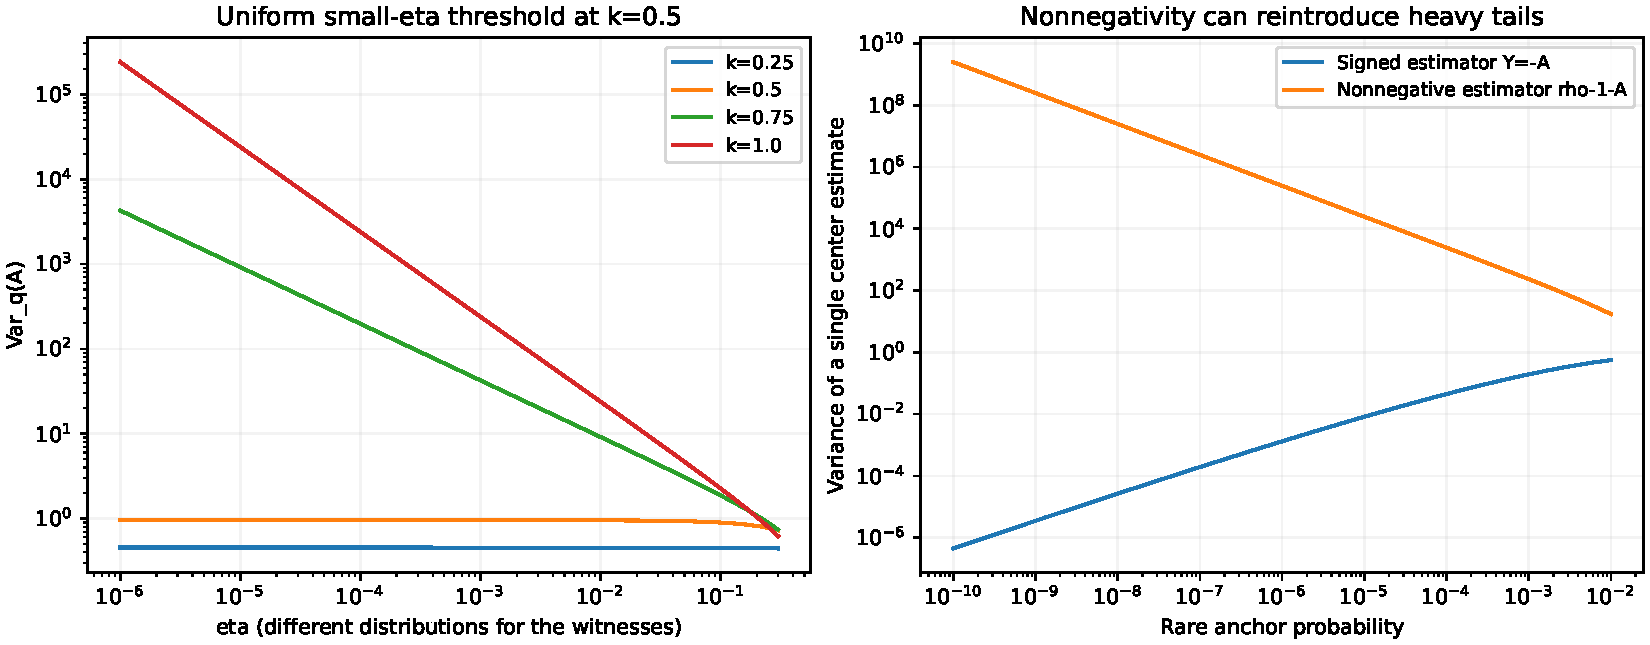
\includegraphics[width=\textwidth]{../../results/power-center-advantage/small-step-and-estimation.pdf}
 \caption{左：小步方差阈值的下界见证，不同形状使用不同分布族，不能当作同数据上的性能排名。右：逐样本非负中心估计可能重新引入概率比重尾。}
\end{figure}
\begin{figure}[htbp]
 \centering
 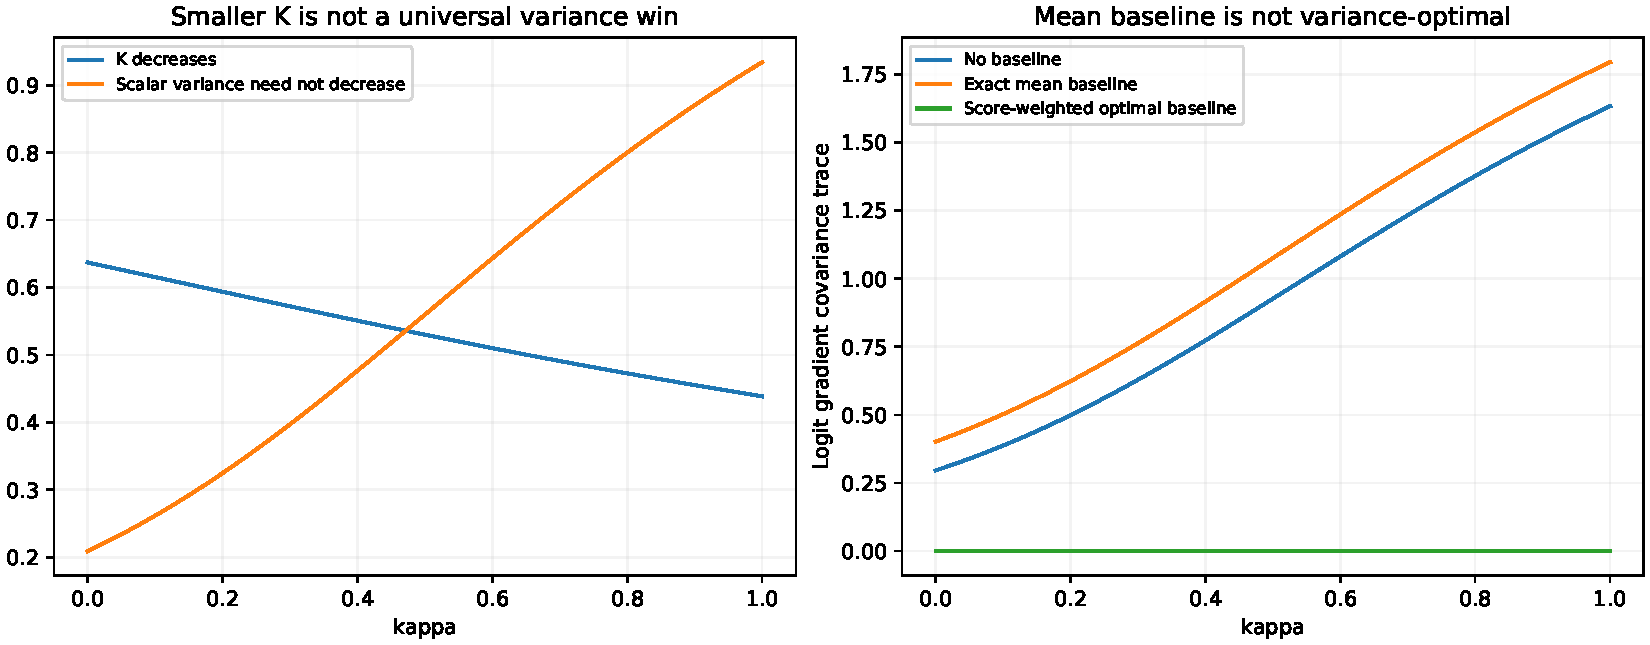
\includegraphics[width=\textwidth]{../../results/power-center-advantage/baseline-counterexample.pdf}
 \caption{同一二元输入下，$K$ 随形状下降但标量方差不必下降；均值 baseline 也不一定降低 logit 梯度方差。零方差最优 baseline 是二元例子的性质，不是一般网络结论。}
\end{figure}

数学核验与真实缓存审计见 \path{experiments/analysis/power_center_advantage.py}；真实缓存取原 64 条 t22 response 每条两个固定随机 reservoir 位置，共 128 个 prefix，对 20 组 $\kappa,\eta$ 精确求 action 条件矩。结果与所有实验统一维护在唯一实验报告；这些 CPU 模型分布统计不等于新 GPU 训练或全参数梯度方差。

下面继续在同一冻结前缀上改进 $K$ 的辅助 action 估计。除专门的 logits 结论外，所有向量方差均指协方差 trace，参数固定，动作来自同一 prefix 的独立条件抽样。辅助 action 不等于新增完整 response；对不同 prefix 的 token 套用本节协方差公式会改变目标。

\subsection{一般混合提案的样本上界与输入方差最优性}

记 $\rho=T/q$、$\phi=\rho-1-A$、$c=-\log(1-\eta)/(\kappa\eta)$，这里 $\kappa>0$、$\eta<1$，所以 $c>1$。对任意 $0<\zeta<1$，取 $\mu_\zeta=(1-\zeta)q+\zeta T$、$Z_\zeta=\phi/(1-\zeta+\zeta\rho)$。它对 $K$ 无偏。由 $0\le\phi(x)\le x+c-1$，
\begin{equation}
 0\le Z_\zeta\le C_\zeta,
 \qquad C_\zeta=\max\{(c-1)/(1-\zeta),1/\zeta\}.
\end{equation}
这个上界是逐概率比的精确上确界：$x\to0$ 时 $\phi(x)\to c-1$；$x\to\infty$ 时 $\phi(x)/x\to1$，两个端点分别达到上述两项。第一项随 $\zeta$ 增加、第二项随 $\zeta$ 减少，唯一最小最大值发生在 $\zeta=1/c$，值为 $c$。这解释前节提案的选择，不表示其每个输入的方差最小。

固定输入的方差为
\begin{equation}
 W(\zeta)=\E_q\frac{\phi(\rho)^2}{1+\zeta(\rho-1)}-K^2,
 \qquad W''(\zeta)=2\E_q\frac{\phi(\rho)^2(\rho-1)^2}{[1+\zeta(\rho-1)]^3}\ge0.
\end{equation}
因此可以做一维凸优化选择输入方差最优混合权重；它可以落在端点，也可以不同于 $1/c$。随机 pilot 选权重时，后续样本应与选权重的数据独立，或给出适应性修正。更小的输入方差与更小的统一样本范围是不同目标。
\subsection{把 head--tail 区间变成有界无偏估计器}

令 head 为 $S$、尾部为 $C$，$\delta=\sum_Cq$、$\tau_T=\sum_CT$，假设 $\delta,\tau_T>0$。定义 $r_0=\tau_T/\delta$、$H=\sum_Sq\phi(\rho)$。上一小节的确定性区间可改写为
\begin{align}
 L&=H+\delta\phi(r_0),\\
 U&=H+\tau_T+(c-1)\delta,\\
 w&=U-L=\delta[c+A(r_0)].
 \label{eq:center-tail-interval-lu}
\end{align}
我们可以使随机估计值始终位于这个区间，同时保持无偏。

对尾部概率比定义凸余项
\begin{align}
 g(x)&=\phi(x)-\phi(r_0)-\phi'(r_0)(x-r_0)\\
 &=-A(x)+A(r_0)+A'(r_0)(x-r_0),\\
 u&=A'(r_0)=\frac{r_0^{\kappa-1}}{1-\eta+\eta r_0^\kappa},\qquad
 v=c+A(r_0)-r_0u.
\end{align}
凸性给出 $g\ge0$，且 $A\ge-c$ 给出 $g(x)\le ux+v$。$u>0$；$A$ 凹且 $A(0)=-c$，在 $r_0$ 处的切线于零点的截距 $A(r_0)-r_0A'(r_0)$ 不低于 $-c$，所以 $v\ge0$。尾部中 $\sum_Cq(\rho-r_0)=0$，故
\begin{equation}
 \sum_Cqg(\rho)=K-L,\qquad u\tau_T+v\delta=w.
\end{equation}
当 $w>0$，取仅支持尾部的提案和估计值
\begin{equation}
 \nu(a)=\frac{uT_a+vq_a}{w},\qquad
 Y(a)=\frac{q_ag(\rho_a)}{\nu(a)},\quad a\sim\nu.
\end{equation}
由 $g\le u\rho+v$，有 $0\le Y\le w$。提案可通过条件尾部分布抽样：以概率 $u\tau_T/w$ 从 $T(\cdot\mid C)$ 抽一个 action，否则从 $q(\cdot\mid C)$ 抽一个 action。其响应 rollout 测度仍为 $q$。

\begin{theorem}[区间内的无偏教师中心估计]
\label{thm:center-tail-bounded-estimator}
令 $Y_1,\ldots,Y_M$ 为上述独立尾部样本，$\widehat K=L+M^{-1}\sum_iY_i$。则
\begin{align}
 \E\widehat K&=K,\qquad L\le\widehat K\le U,\\
 \Var\widehat K&\le\frac{(K-L)(U-K)}M\le\frac{w^2}{4M},\\
 \Pr(|\widehat K-K|\ge\epsilon)&\le2\exp(-2M\epsilon^2/w^2).
\end{align}
若 $w=0$ 或尾部为空，直接返回确定的 $K=L=U$。
\end{theorem}

\begin{proof}
尾部余项的恒等式给出 $\E_\nu Y=K-L$，所以均值正确。逐样本范围给出 $Y^2\le wY$，因此 $\Var Y\le w(K-L)-(K-L)^2=(K-L)(U-K)$。独立平均除以 $M$，并用 Hoeffding 得到最后一式。$L\ge0$ 是粗粒化的凸散度，故估计非负。\hfill$\square$
\end{proof}

估计需要能够从条件尾部分布抽样并读取抽中 action 的 $q_a,T_a$。仅有 head 与两种尾部质量时，不能无偏还原 $K$：保持全部已知量不变，让尾部 $T/q$ 恒定得到下界 $L$，将教师尾部质量偏向一个 action 则由严格凸性得到更大的 $K$。仅依赖已知量的随机估计器对两种输入具有相同期望，不能同时无偏。若完整 logits 已经可用，精确求和通常更直接；稀疏缓存模式需把尾部查询成本纳入比较。

无 head 时，$\delta=\tau_T=r_0=1$、$u=1$、$v=c-1$、$L=0$、$w=c$，精确恢复前节全词表包络估计器。扩大嵌套 head 会缩小 $w$，所以最坏方差和置信宽度保证单调改善；不能据此声称实际输入方差也一定单调改善。若允许至少两个未知尾部 action，在固定 head 和尾部质量下可以令尾部 $q$ 质量集中在 $T/q\to0$ 的 action、$T$ 质量集中在极小 $q$ 的另一个 action，使 $K\to U$。任何无偏、非负的残差估计器若有统一样本上界 $b$，都需 $b\ge\sup(K-L)=w$；本构造达到这个信息条件下的统一范围。

还有一个容易实现的备选：直接估计尾部 $\sum_Cq\phi$，使用提案 $(T+(c-1)q)/[\tau_T+(c-1)\delta]$ 在尾部条件化，再加精确 head。固定此包络时，逐步扩大 head 的实际估计方差也不增加：若原提案落入新尾部的概率为 $p_C$，新估计方差为 $p_C^2\Var(Z\mid C)$，原方差由全方差公式至少为 $p_C\Var(Z\mid C)$。但该备选的随机值不保证高于更强的 Jensen 下界 $L$。两种估计分别提供实际方差单调性与更紧的逐样本区间，不混用结论。

\subsection{缓存教师中心误差与末期噪声}

记 $h=U-f$、$R=C_qh$、$D=R/\eta$、$\psi=\nabla\log p$、$\varphi=\psi-\E_q\psi$。真实 BPO 梯度为 $\bm G=\E_qD\psi=\E_qD\varphi$。若缓存 $\widehat K=K+e$，使用未修正的 score 更新会产生偏差 $-e\E_q\psi$。改用中心化 score 后，任意固定 $e$ 都不改变梯度期望，却保留随机性。尤其在 $p=m$，$D=0$，
\begin{equation}
 g=-e\varphi,\qquad
 \Var_q(g)=e^2\E_q\|\varphi\|^2.
\end{equation}
若中心用 $M$ 个独立样本估计、方差为 $\sigma_K^2/M$，再对中心误差求平均，就得到 $\sigma_K^2\E_q\|\varphi\|^2/M$ 的末期噪声。完整条件求和时，$\E_q\varphi=0$ 会精确消掉这一项；因此完整词表 BPO 不需要通过教师中心估计器控制这一采样噪声来源。

可以利用学生反馈估计中心：令 $y=C_qU/\eta-A$，则 $\E_qy=K$，而
\begin{equation}
 \Var_qy=\Var_qD=\frac{2\mathcal L_{\mathrm{BPO}}}{\eta}.
\end{equation}
独立辅助 action 上的 $y$ 估计在拟合到 target 时方差消失，优于仅依靠 teacher 监督的固定中心噪声底；它通常没有逐样本统一范围。下面将这个差分进一步对称化，同时消去学生条件中心。
\subsection{不显式估计两个中心的 BPO 二样本损失}

令 $a,b\overset{\mathrm{iid}}\sim q$，定义
\begin{equation}
 \widehat\ell_2=\frac{[h(a)-h(b)]^2}{4\eta},\qquad
 \widehat{\bm G}_2=\frac{[h(a)-h(b)][\psi(a)-\psi(b)]}{2\eta}.
 \label{eq:center-free-pair-bpo}
\end{equation}
方差的二样本恒等式给出 $\E\widehat\ell_2=\Var_qh/(2\eta)=\mathcal L_{\mathrm{BPO}}$。直接微分样本平方差得到所列梯度，且
\begin{align}
 \E[(h-h')(\psi-\psi')]&=2[\E h\psi-(\E h)(\E\psi)],\\
 \E\widehat{\bm G}_2&=\nabla\mathcal L_{\mathrm{BPO}}.
\end{align}
这保留 BPO population 目标，而非把非负 $K$ 估计与同一 action 相加造成的形状消失。

令 logits 为 $z$。两种条件归一化常数均在差分中消失：
\begin{equation}
 h(a)-h(b)=z(a)-z(b)-\log(q_a/q_b)-[f(a)-f(b)].
\end{equation}
因此既不需要 $K$，也不需要 $\E_qU$ 或 $\E_q\psi$。$\psi(a)-\psi(b)=\nabla[z(a)-z(b)]$，学生 softmax 归一化也不必进入损失。对任意 logits 和 target log 权重的常数平移，样本损失不变。

对 $M\ge2$ 个 iid $q$ action，可使用所有样本对的 U 统计量，即无偏样本方差损失
\begin{align}
 \bar h&=M^{-1}\sum_{i=1}^Mh_i,\\
 \widehat{\mathcal L}_M
 &=\frac{\sum_i(h_i-\bar h)^2}{2\eta(M-1)},\\
 \nabla\widehat{\mathcal L}_M
 &=\frac{\sum_i(h_i-\bar h)\psi_i}{\eta(M-1)}.
 \label{eq:center-free-sample-variance-bpo}
\end{align}
因为样本偏差和为零，中心导数逐样本消掉。分母必须是 $M-1$；采用 $M$ 会把期望损失和梯度缩小为 $(M-1)/M$ 倍。$M=1$ 不定义该方差损失。这里是同一条件分布的辅助 token 抽样，不是 response 候选组、后缀 reward 或随机标准差归一化。

在任意 $p=m$ 处，$h$ 对全部 action 为常数，故每个有限样本损失和梯度都为零。若 $\|\psi(a)\|\le S$，则
\begin{align}
 \E\|\widehat{\bm G}_2\|^2
 &\le\frac{S^2}{\eta^2}\E(h-h')^2
 =\frac{4S^2}{\eta}\mathcal L_{\mathrm{BPO}}.
\end{align}
因此这个估计器拥有误差相关噪声控制，不需要假设教师中心先被精确估计；$\kappa=0$ 也成立。正形状另外控制 initial 教师尾部。该结论需精确抽样、固定参数和统一 score 条件。
\subsection{相同 action 预算下的方差代价}

记精确中心化 score 估计器 $g_c=(h-\E_qh)(\psi-\E_q\psi)/\eta$，其方差为 $V_c$；二样本核 $\widehat{\bm G}_2$ 的方差为 $V_2$。设 $H_1(a)=\E_b\widehat{\bm G}_2(a,b)-\bm G$。展开上式得到 $H_1=(g_c-\bm G)/2$，所以 $\Var H_1=V_c/4$。减去两个一阶项的核 $H_2(a,b)=\widehat{\bm G}_2-\bm G-H_1(a)-H_1(b)$ 具有零条件均值，其方差为 $V_2-V_c/2\ge0$。

对所有样本对平均时，独立零条件均值核之间即使共享一个索引也正交；一阶项与二阶项也正交。因此逐项计算协方差 trace 给出
\begin{align}
 \Var(\nabla\widehat{\mathcal L}_M)
 &=\frac{4}{M}\Var H_1+\frac{2}{M(M-1)}\Var H_2\\
 &=\frac{(M-2)V_c+2V_2}{M(M-1)},\\
 \Var(\nabla\widehat{\mathcal L}_M)-\frac{V_c}{M}
 &=\frac{2V_2-V_c}{M(M-1)}\ge0.
 \label{eq:center-free-variance-cost}
\end{align}
所以它不会在相同 $M$ action 预算下击败已经知道精确两中心的这个 oracle 估计器；优势是取消两中心计算、保持无偏和实现零误差零样本梯度。代价是 $O(M^{-2})$ 的额外方差。学生 score 加权最优 baseline 还可能优于这里的精确均值中心，不据此宣称全局最优。

独立 categorical logits 有特别清楚的恒等式。令 $V_h=\Var_qh/\eta^2$、$\bm G=q\odot C_qh/\eta$、$Q_2=\sum_aq_a^2$，则
\begin{align}
 \E\|\widehat{\bm G}_2\|^2&=V_h=2\mathcal L_{\mathrm{BPO}}/\eta,\\
 V_2&=V_h-\|\bm G\|^2,\qquad
 V_c=(1+Q_2)V_h-3\|\bm G\|^2.
\end{align}
第一式利用不同 action 的 $\|e_a-e_b\|^2=2$，相同 action 的差分为零。inner 起点 $V_h$ 就是教师 advantage 方差。因而前节 $\kappa_\star\simeq0.441928$ 的锐小步常数同时控制二样本 logits 梯度的最坏二阶矩；这不是共享网络梯度信噪比结论。把每个 action 均匀复制为 $N$ 个同概率比子 action，$V_h$ 不变、$Q_2$ 与 $\|\bm G\|^2$ 各除以 $N$，于是 $V_2\to V_h$、$\Var(\nabla\widehat{\mathcal L}_M)\to V_h/(M-1)$。这提供高维方差代价的直观极限，不把最优形状结论直接推广到任意固定维数和任意模型。
\subsection{冻结混合提案下的有界重要性校正}

二样本 BPO 还可以改变辅助 action 提案，保持 response 的行为分布 $q$ 不变。令 $\mu=(1-\zeta)q+\zeta T$、$0<\zeta<1$，定义 $w_a=q_a/\mu_a$。对 $a,b\overset{\mathrm{iid}}\sim\mu$，取
\begin{equation}
 \widehat\ell_{2,\mu}=w_aw_b[h(a)-h(b)]^2/(4\eta).
\end{equation}
$q,T,\mu$ 在本轮冻结，权重停止梯度。逐样本对的 $\mu_a\mu_bw_aw_b=q_aq_b$ 保证 $\E_\mu\widehat\ell_{2,\mu}=\mathcal L_{\mathrm{BPO}}$，梯度也无偏；$M$ action 使用全部加权样本对的 U 统计量即可。不能把样本权重除以随机总和，否则不再是上述无偏估计器。

由 $\mu\ge(1-\zeta)q$，有 $w\le1/(1-\zeta)$。取 $\zeta=1/2$ 时，单 action 权重不超过 2，样本对权重不超过 4，无需裁剪。拟合到 target 时，差分仍逐样本为零。在相同 score 条件下，二阶矩满足
\begin{equation}
 \E_\mu\|w_aw_b\widehat{\bm G}_2\|^2
 =\E_{q\otimes q}[w_aw_b\|\widehat{\bm G}_2\|^2]
 \le\frac{4S^2}{\eta(1-\zeta)^2}\mathcal L_{\mathrm{BPO}}.
\end{equation}
这个最坏界可能更松，固定输入的实际方差却可以更小。二元 $q=(\epsilon,1-\epsilon)$、$T=(1-\epsilon^2,\epsilon^2)$ 中，当 $h(1)\ne h(2)$ 时，非零二样本 logits 梯度只出现在两个 action 不同时。$q$ 提案下相对方差为 $[2\epsilon(1-\epsilon)]^{-1}-1$，随 $\epsilon\to0$ 发散，且只要监督差非零便与 $\kappa$ 的整体尺度无关。混合提案的重要性校正梯度仍只在不同 action 时非零，该事件概率为 $2\mu_1(1-\mu_1)$，故相对方差为 $[2\mu_1(1-\mu_1)]^{-1}-1$；当 $\zeta=1/2$、$\epsilon\to0$ 时趋于 1。这个反例展示绝对方差小并不意味着信噪比好，提案调整可以解决部分稀有 action 抽样问题。它不保证每个输入或共享网络都改善。
\subsection{排除重复 action 的参数协方差改进}

独立二样本在 $a=b$ 时没有损失或梯度，却消耗两次 action 评估。可以直接改为 $a\sim q$、$b\sim q(\cdot\mid b\ne a)$，并使用
\begin{equation}
 \widehat\ell_{\mathrm{nr}}=(1-q_a)[h(a)-h(b)]^2/(4\eta),\qquad
 \widehat{\bm G}_{\mathrm{nr}}=(1-q_a)\widehat{\bm G}_2(a,b).
\end{equation}
这里是有序条件抽样，不是随意挑选不同 token。其联合概率为 $q_aq_b/(1-q_a)$，对角核为零，所以损失和梯度的期望都与原 BPO 相同；校正权重自然在 $[0,1]$ 内，不需要裁剪。

不仅协方差 trace 会下降，整个参数梯度协方差矩阵也有半正定序保证。两种估计的均值均为 $\bm G$，而
\begin{align}
 \E_{\mathrm{nr}}[\widehat{\bm G}_{\mathrm{nr}}\widehat{\bm G}_{\mathrm{nr}}^\top]
 &=\E_{q\otimes q}[(1-q_a)\widehat{\bm G}_2\widehat{\bm G}_2^\top],\\
 \operatorname{Cov}_{q\otimes q}(\widehat{\bm G}_2)
 -\operatorname{Cov}_{\mathrm{nr}}(\widehat{\bm G}_{\mathrm{nr}})
 &=\E_{q\otimes q}[q_a\widehat{\bm G}_2\widehat{\bm G}_2^\top]\succeq0.
\end{align}
这对任意固定参数的神经网络 Jacobian 都成立，不限于独立 logits；要求精确条件概率、抽样和数值梯度。相同两个 action 预算下，它在每个参数方向的方差都不增加。实际浮点误差与有限抽样的协方差估计仍需测量，不能把八次探针的随机排名当成证明。

categorical logits 的 trace 可直接写为 $V_{\mathrm{nr}}=(1-Q_2/2)V_h-3\|\bm G\|^2/2$。与独立二样本相比减少 $(Q_2V_h+\|\bm G\|^2)/2$。该改进不改变 $q$ 加权回归的条件数，不消除稀有 action 的所有困难，也不意味着 AdamW 训练效果必然改善。
\subsection{样本复用的图 Laplacian 与实验范围}

冻结一个 prefix 的有限 action 样本反复训练时，把词表视为图节点、抽到的不同 action 对视为边。样本损失是 $z-\log m$ 的图 Laplacian 二次型。连通分量内相等的误差都给出零损失；只有图连通到完整支持时，零样本损失才强制全局 $p=m$。一个 frozen pair 只约束一个 log-odds，不能识别完整 target。

在当前 $\theta$ 固定后重新抽 $M\ge2$ 个 iid $q$ action，才保留条件无偏 population 梯度；不需要重新生成 response。使用 rollout token 配一个辅助 token时，需额外检查该 token 的抽样条件和前缀权重是否可预测。继续复用有限 action 集则优化其真实 empirical loss，但不宣称条件无偏或零样本损失等于完整 target 已解完。

若教师重新查询昂贵，可以在冻结 $q$ 后预抽样独立 action tape，对每个前缀的第 $j$ 次 inner 缓存 $M$ 个 action 的 $\log q$ 和 $f$，按顺序各使用一次。当前参数只依赖已用样本，未用 tape 对它保持条件独立；不能用未来样本结果选择更新或重用同一 tape 块后继续宣称无偏。训练损失只需要选中 logits 与这些冻结 log 权重，存储量为每 prefix 的 $O(IM)$，不必存完整 $O(|\mathcal V|)$ target。原完整词表 teacher forward 是否因此变快还需专项实现与测量，存储计数本身不能证明吞吐收益。

这些估计器的区别是目标、无偏条件、同 action 预算方差与所需查询接口。已有模型缓存统计见实验总报告；GPU 训练计划不作为本节理论证明的一部分。

\begin{figure}[htbp]
 \centering
 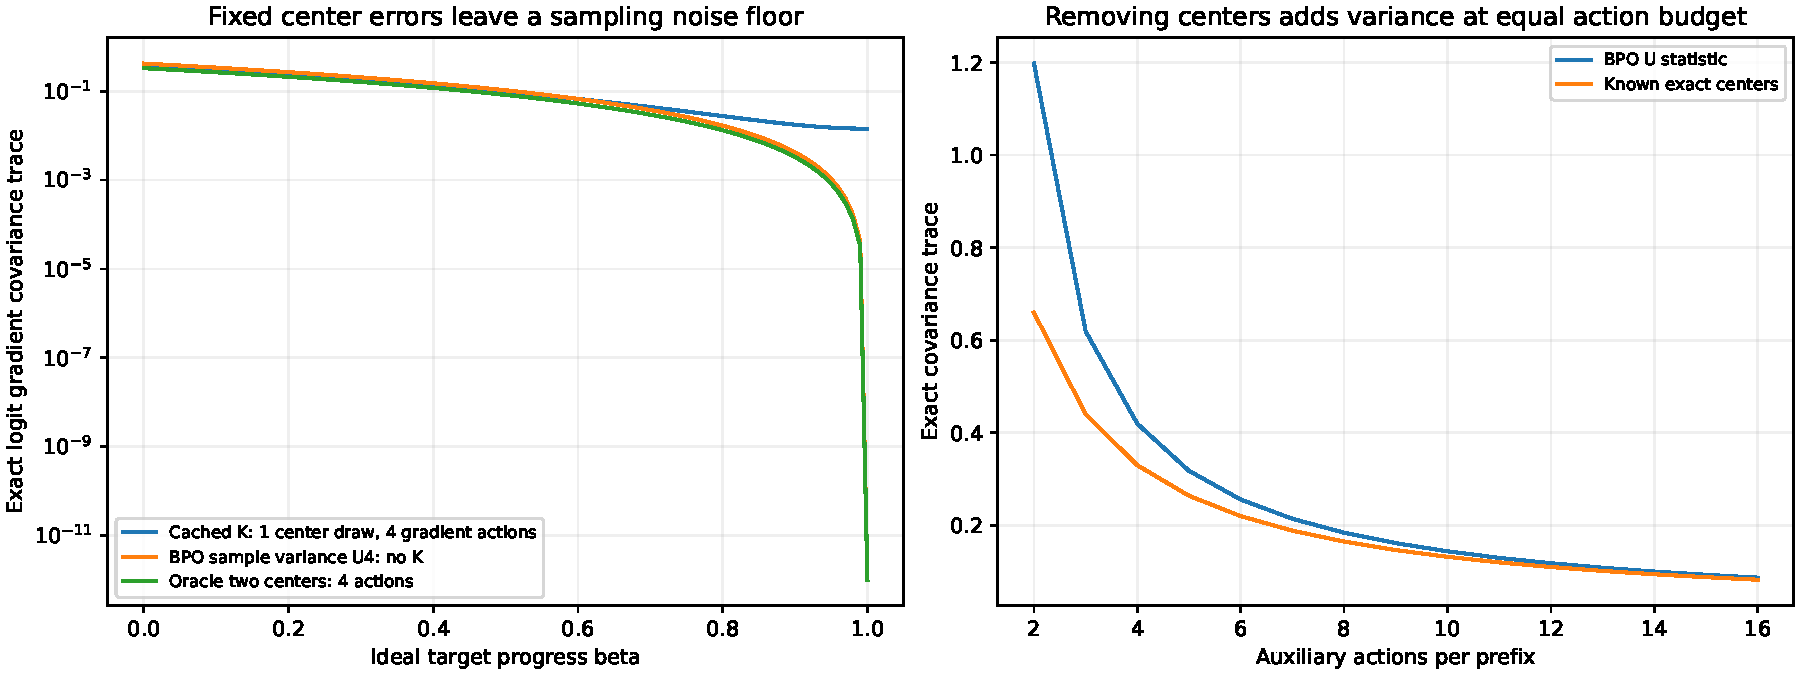
\includegraphics[width=\textwidth]{../../results/power-center-extensions/center-noise-and-sample-variance.pdf}
 \caption{理想 logits 拟合路径上，固定教师中心估计产生末期采样噪声底；BPO sample-variance 梯度的方差随残差平方下降。右图按相同辅助 action 数比较，取消两中心计算有额外方差代价。}
\end{figure}
\begin{figure}[htbp]
 \centering
 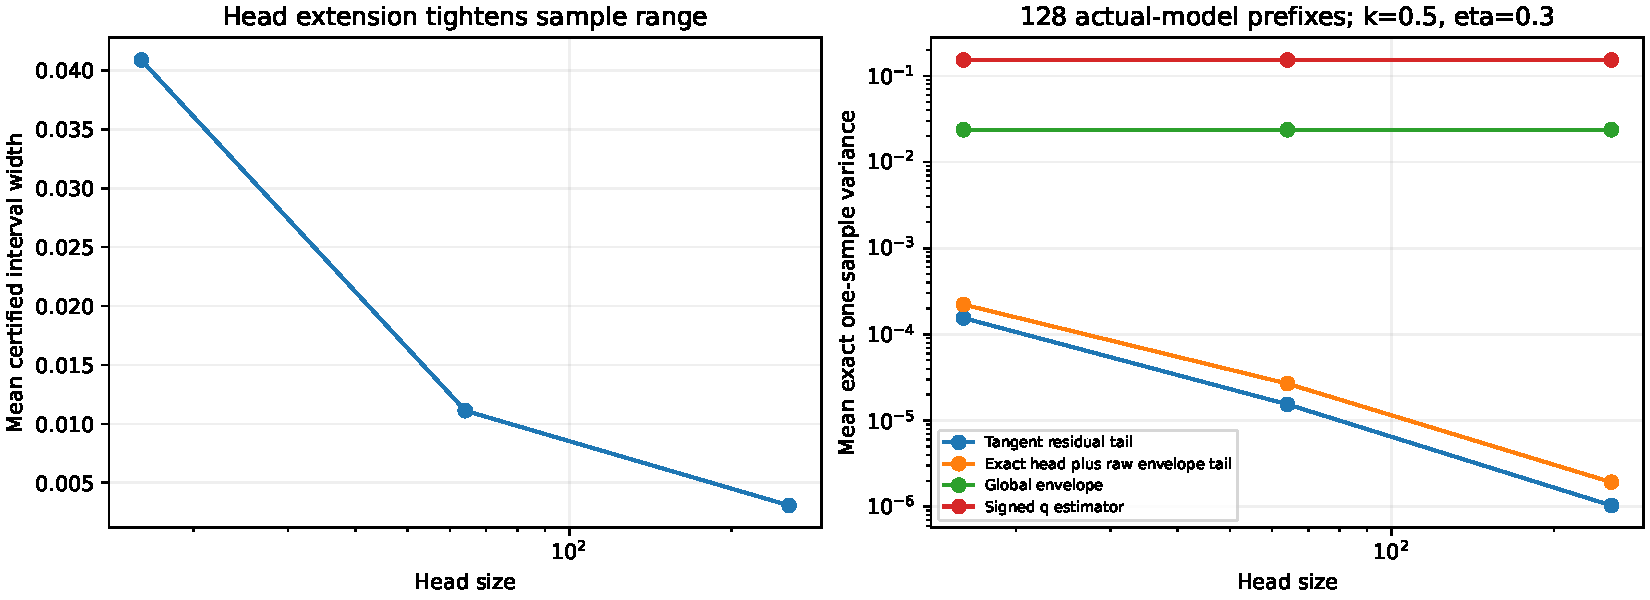
\includegraphics[width=\textwidth]{../../results/power-center-extensions/cached-head-tail-estimation.pdf}
 \caption{原模型缓存 128 个固定前缀上的 tail 区间与无偏估计器条件矩。扩大 head 收紧统一范围与置信保证；实际方差按数据读出，不声称所有输入上都优于其他估计器。}
\end{figure}


\section{高维动力学、投影与其他拟合目标}
\label{sec:power-projection}
\subsection{概率坐标、log-odds 与高维方向}

词表维数为 $d$ 时，每个前缀的 token 分布位于 $\Delta^{d-1}$。算术 target $m_{1,\eta}=(1-\eta)q+\eta T$ 在概率坐标中是直线。几何 target $m_{0,\eta}\propto q^{1-\eta}T^\eta$ 的 log-odds 则满足
\begin{equation}
 \log\frac{m_{0,\eta,a}}{m_{0,\eta,b}}
 =(1-\eta)\log\frac{q_a}{q_b}+\eta\log\frac{T_a}{T_b}.
\end{equation}
归一化常数在坐标差中消失；因此几何 target 在 log-odds 中是直线。这对应信息几何中的 mixture 路径和 exponential 路径\footnote{Shun-ichi Amari. Information Geometry and Its Applications: Convex Function and Dually Flat Manifold. ETVC 2008, LNCS 5416, 2009, pp. 75--102. \url{https://bsi-ni.brain.riken.jp/database/file/293/299.pdf}.}。当 teacher 极小概率接近零时，几何 target 的对应概率也可接近零，即使 $\eta$ 固定得很小；算术 target 则保留 $(1-\eta)q_a$ 的概率下界。

对 $\eta$ 在零处求导，两个方向分别为
\begin{equation}
 \left.\partial_\eta m_{1,\eta}\right|_{\eta=0}=T-q,\qquad
 \left.\partial_\eta m_{0,\eta,a}\right|_{\eta=0}
 =q_a[\log(T_a/q_a)-\E_q\log(T/q)].
\end{equation}
第一式是概率插值的直接微分。第二式使用未归一化几何密度的导数 $q_a\log(T_a/q_a)$，再减去配分函数导数对应的条件均值。高维下两方向一般不共线；统一缩放步长不能纠正方向差异。只有全部 teacher/anchor 比率一致接近一时，$\log\rho=\rho-1+O((\rho-1)^2)$ 才使两方向一阶接近。

\subsection{从 TOP-D 的证明到可验证的泛化}

TOP-D 的三个理论对象是即时奖励乘 score 的二阶矩、算术分布算子的收缩，以及固定奖励 MDP 的性能下界。前两者不能单独保证神经网络的有限 inner 优化或整条 response 的 KL 下降。本节保留有限词表、完整支持和单个固定 teacher，进一步连接精确 target、内层拟合、共同评价散度与轨迹访问测度。所有新增结论在实验前先用解析证明和数值恒等式核验；真实模型的矩测量用于检验实际常数，不替代证明。

\subsection{精确幂均值步降低所有凸生成散度}

令 $s_a=q_a/t_a$。幂均值 target 可写为 $m_a=t_aG(s_a)/Z$，其中
\begin{equation}
 G(s)=[(1-\lambda)s^\kappa+\lambda]^{1/\kappa},\quad
 G_0(s)=s^{1-\lambda},\quad Z=\E_tG(s).
\end{equation}
$G$ 严格递增，$G(s)/s$ 严格递减。对 $\kappa>0$，第二条由
\begin{equation}
 \frac{d}{d\log s}\log\frac{G(s)}s
 =-\frac{\lambda s^{-\kappa}}{1-\lambda+\lambda s^{-\kappa}}<0
\end{equation}
得到；几何端点导数为 $-\lambda$。又有 $Z=\sum_aq_a[G(s_a)/s_a]$，故存在 $s_\star\in[\min s,\max s]$ 使 $G(s_\star)/s_\star=Z$。若 $s_a<s_\star$，则 $s_a\le G(s_a)/Z\le s_\star$；若 $s_a>s_\star$，则 $s_\star\le G(s_a)/Z\le s_a$。

\begin{theorem}[单教师的凸生成散度单调性]
\label{thm:proximal-all-f-divergences}
对任意凸函数 $\varphi:(0,\infty)\to\R$、$\varphi(1)=0$，定义 $D_\varphi(q\Vert t)=\sum_at_a\varphi(q_a/t_a)$。精确 target 满足 $D_\varphi(m\Vert t)\le D_\varphi(q\Vert t)$。因此 $\KL(m\Vert t)$、$\KL(t\Vert m)$、Hellinger 散度、TV 和 $\chi^2(m\Vert t)$ 同时不增加。
\end{theorem}

\begin{proof}
取 $c\in\partial\varphi(s_\star)$。凸函数 $\varphi(s)-cs$ 在 $s_\star$ 取得最小值，且在其两侧分别单调不增、单调不减。每个 $s_a'=m_a/t_a=G(s_a)/Z$ 都位于 $s_a$ 与 $s_\star$ 之间，因此 $\varphi(s_a')-cs_a'\le\varphi(s_a)-cs_a$。乘以 $t_a$ 并求和，由 $\sum_at_as_a'=\sum_at_as_a=1$，线性项抵消，得结论。\hfill$\square$
\end{proof}

这个结论比各自 $D_\kappa$ 的单调性更强，但只直接覆盖精确 target。它并不声称有限 inner 只要降低任何一个拟合损失，就自动同时改善所有散度。

\subsection{保持 teacher 的可逆 Markov 核}

还可构造一个依赖 $q,t$ 的转移核 $K$，满足 $tK=t$、$qK=m$。令 $\delta_a=m_a-q_a$，$L=\{a:\delta_a>0\}$、$H=\{b:\delta_b<0\}$，以及 $D=\sum_{a\in L}\delta_a=\sum_{b\in H}(-\delta_b)$。$D=0$ 时取 $K=I$。否则，对 $a\in L,b\in H$ 定义
\begin{equation}
 w_{ab}=w_{ba}=\frac{\delta_a(-\delta_b)}{D(s_b-s_a)},\qquad
 K_{ab}=w_{ab}/t_a,\quad K_{ba}=w_{ab}/t_b,
\end{equation}
其余非对角项为零，$K_{aa}=1-\sum_{b\ne a}K_{ab}$。由共同交点性质，$a\in L$ 时 $\delta_a/t_a\le s_\star-s_a$，$b\in H$ 时 $(-\delta_b)/t_b\le s_b-s_\star$。所以
\begin{equation}
 \sum_{b\in H}w_{ab}\le\frac{\delta_a}{s_\star-s_a}\le t_a,\qquad
 \sum_{a\in L}w_{ab}\le\frac{-\delta_b}{s_b-s_\star}\le t_b.
\end{equation}
对角项非负，行和为一；$t_aK_{ab}=t_bK_{ba}$ 保证详细平衡与 $tK=t$。对 $a\in L$，$(qK)_a-q_a=\sum_b w_{ab}(s_b-s_a)=\delta_a$；对 $b\in H$ 同样得到其损失质量，故 $qK=m$。

由 $m_j/t_j=\sum_i(t_iK_{ij}/t_j)s_i$ 与 Jensen 不等式，也能重新证明上一条定理。这个核是精确更新的数学表示，不要求实际构造一个词表大小平方的矩阵。它给出共同 teacher 下的保序质量转移解释，避免仅凭某个特定 KL 方向描述更新。

\subsection{目标半径随插值强度单调}

固定 $q,t,\kappa$，记 $m_\lambda$ 为 target。对 $0<\lambda_1<\lambda_2<1$，$m_{\lambda_1}/q$ 随 $\rho=t/q$ 严格递增，且
\begin{equation}
 \frac{m_{\lambda_2,a}}{m_{\lambda_1,a}}
 =\frac{Z_{\lambda_1}}{Z_{\lambda_2}}
 \left(\frac{1-\lambda_2+\lambda_2\rho_a^\kappa}
 {1-\lambda_1+\lambda_1\rho_a^\kappa}\right)^{1/\kappa}
\end{equation}
也随 $\rho_a$ 严格递增。几何端点对应 $Z_{\lambda_1}\rho_a^{\lambda_2-\lambda_1}/Z_{\lambda_2}$。取两条比率相等的共同交点，$m_{\lambda_2}/q$ 相对 $m_{\lambda_1}/q$ 在低端进一步减小、高端进一步增大。用上一条定理的支撑直线证明反向不等式，得到
\begin{equation}
 D_\varphi(m_{\lambda_2}\Vert q)\ge D_\varphi(m_{\lambda_1}\Vert q).
\end{equation}
$\lambda_1=0$ 时由散度非负性成立。取 $\varphi(s)=(\sqrt s-1)^2$，得 Hellinger 距离与 Fisher--Rao 距离随 $\lambda$ 单调。对不同 prefix 的固定加权平均也成立。因此可以在指定前缀面板上唯一校准共同的目标半径，而不是假设相同 $\lambda$ 自动等于相同步幅。校准面板与实际比较面板不同时，半径还须在比较面板上独立读出。

\subsection{有限 inner 的 reverse KL 与 Rényi 证书}

令 $\epsilon=\KL(p\Vert m)$、$A(a)=\log(m_a/t_a)$，$H=\max A-\min A$。恒等式为
\begin{equation}
 \KL(p\Vert t)=\epsilon+\KL(m\Vert t)+\sum_a(p_a-m_a)A(a).
\end{equation}
减去 $A$ 的区间中点后使用 Hölder 和 Pinsker 不等式，得到
\begin{equation}
 \KL(p\Vert t)\le\KL(m\Vert t)+\epsilon+H\sqrt{\epsilon/2}.
 \label{eq:proximal-range-certificate}
\end{equation}
若右侧不超过 $\KL(q\Vert t)$，则原始 teacher reverse KL 下降。这里 $H$ 可被极小概率的尾部主导，故还需要一个按概率加权的证书。

对任意 $u>0$，令 $r_u(a)=m_a^{1+u}t_a^{-u}/C_u$，$C_u=\sum_am_a^{1+u}t_a^{-u}$。由
\begin{equation}
 \KL(p\Vert r_u)=\epsilon-u\E_pA+\log C_u\ge0,
\end{equation}
得到
\begin{equation}
 \boxed{\KL(p\Vert t)\le
 \inf_{u>0}\left[(1+1/u)\KL(p\Vert m)+D_{1+u}^{\mathrm R}(m\Vert t)\right]},\quad
 D_{1+u}^{\mathrm R}(m\Vert t)=\frac1u\log C_u.
 \label{eq:proximal-renyi-certificate}
\end{equation}
有限个正 $u$ 上取最小值仍是有效上界。$u\to0$ 时，$D_{1+u}^{\mathrm R}(m\Vert t)=\KL(m\Vert t)+\tfrac u2\Var_mA+O(u^2)$。对固定分布、小拟合误差的局部展开，最优平衡项约为 $\sqrt{2\epsilon\Var_mA}$，解释了概率加权证书为何可能比区间界更紧；有限 $u$ 的精确式才是保证。相同 $u$ 下先逐 prefix 应用再固定测度求平均，也能得到整体条件目标的上界。

\subsection{共同目标下的局部最优形状}

令 $r=\log(t/q)$，$w_\kappa=(\rho^\kappa-\E_q\rho^\kappa)/\kappa$，$w_0=C_qr$，于是 $v_\kappa=qw_\kappa$。对固定 Fisher 速度的单位方向 $u_\kappa=v_\kappa/\|v_\kappa\|_F$，reverse KL 的一阶下降量为
\begin{equation}
 -\nabla\KL(q\Vert t)^\top u_\kappa
 =\frac{\E_q[rw_\kappa]}{\sqrt{\E_qw_\kappa^2}}
 \le\sqrt{\Var_qr}.
\end{equation}
这是 Cauchy--Schwarz 不等式，几何形状 $\kappa=0$ 取得等号。对 forward KL，同样有
\begin{equation}
 -\nabla\KL(t\Vert q)^\top u_\kappa
 =\frac{\E_q[\rho w_\kappa]}{\sqrt{\E_qw_\kappa^2}}
 \le\sqrt{\Var_q\rho},
\end{equation}
算术形状 $\kappa=1$ 取得等号。更一般地，$\kappa$ 自己对应的散度具有自己的自然梯度最陡方向。这个局部确定性最优性与平方根形状的最坏矩性质是不同标准，不能由有界方差推出对任何共同评价目标的最优收敛速度。

\subsection{目标自然速度的锐上界与另一个极小极大形状}

对 $0<\kappa<1/2$，令 $X=\rho^\kappa$、$r=1/\kappa>2$，则 $\E_qX^r=1$。$L^p$ 插值不等式给出
\begin{equation}
 \E_qX^2\le(\E_qX)^{(r-2)/(r-1)}
 =(\E_qX)^{(1-2\kappa)/(1-\kappa)}.
\end{equation}
令 $a=\E_qX\in[0,1]$，$\gamma=(1-2\kappa)/(1-\kappa)$。于是 $\Var_qX\le a^\gamma-a^2$。驻点满足 $a^{2-\gamma}=\gamma/2$，代回并记 $b=(1-2\kappa)/[2(1-\kappa)]$，得到锐上界
\begin{equation}
 \boxed{\sup_{q,t}\|v_\kappa\|_F^2
 =C_{\mathrm{vel}}(\kappa)
 =\frac{b^{1-2\kappa}(1-b)}{\kappa^2}}.
\end{equation}
锐性由 $q=(b,1-b)$、$t\to(1,0)$ 达到：$X$ 仅取 $b^{-\kappa}$ 与零，插值不等式和驻点条件同时成立。完整支持分布以极限逼近这个值。$\kappa=1/2$ 的上确界为 4；$\kappa=0$ 或 $\kappa>1/2$ 无有限上界。

在优化 $b$ 后使用包络导数，$d\log C_{\mathrm{vel}}/d\kappa=-2/\kappa-2\log b$。唯一最小点满足
\begin{equation}
 \log\frac{1-2\kappa_\star}{2(1-\kappa_\star)}=-\frac1{\kappa_\star}.
\end{equation}
左侧加 $1/\kappa$ 的导数为 $-1/[(1-2\kappa)(1-\kappa)]-1/\kappa^2<0$，在零点附近趋于正无穷，在 $1/2$ 附近趋于负无穷，故根唯一。根和常数由第一方参考函数 \texttt{minimax\_velocity\_shape}、\texttt{worst\_fisher\_speed\_squared} 计算并验证。

这个最优形状针对 target 的最坏 Fisher 速度上界，与内层误差相关噪声常数的最优 $\kappa_{\mathrm{fit}}=1/2$ 是不同标准。更小的最大速度不自动代表更快学习；部分 teacher 方向也可能变慢。实验将这个由理论确定的 target 作为独立条件，而不把平方根的简洁闭式性质当作通用最优性。

\begin{figure}[htbp]
 \centering
 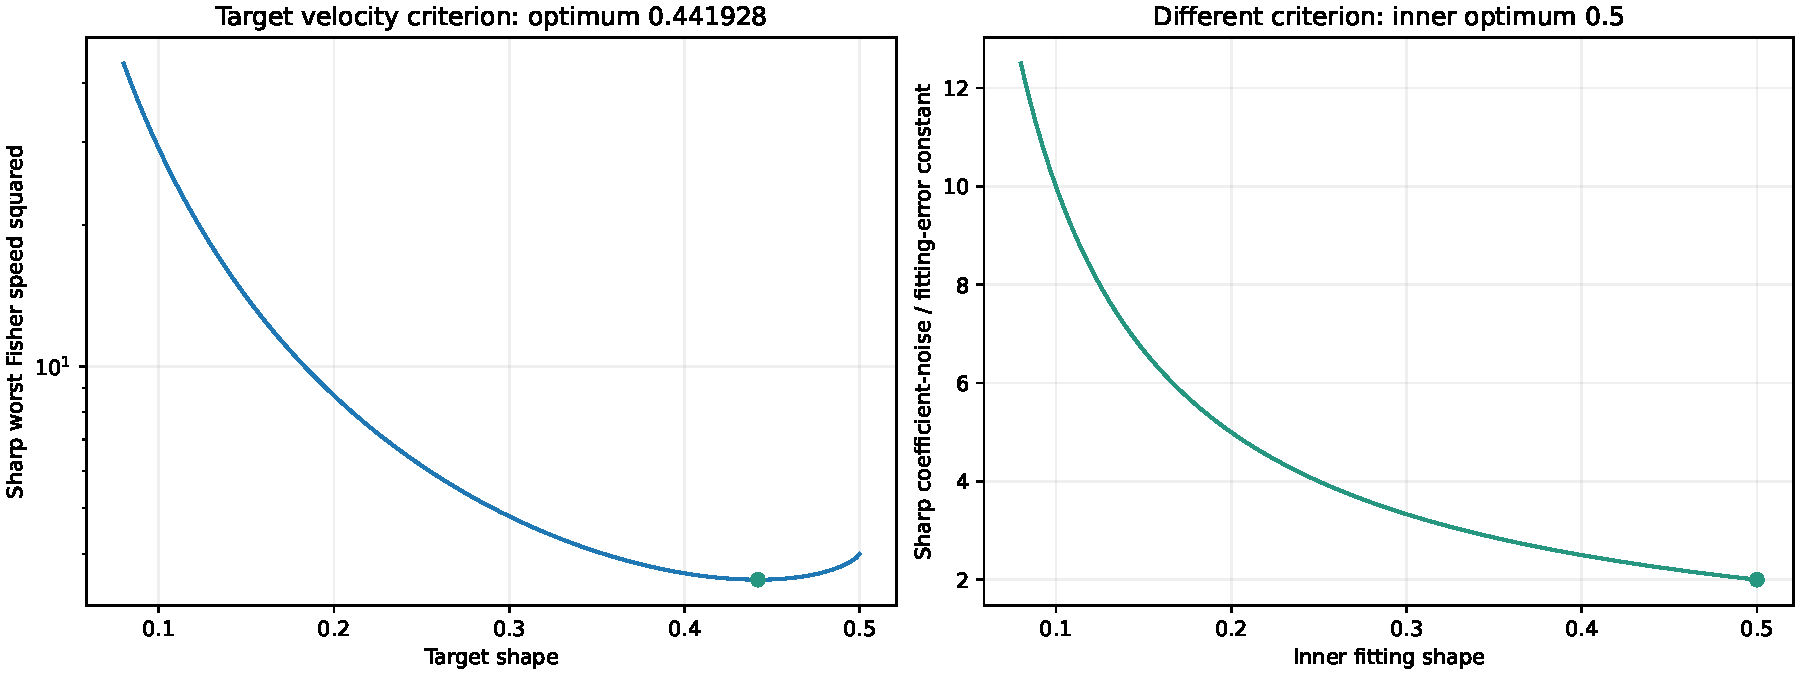
\includegraphics[width=\textwidth]{../../results/power-mean-20261013/two-minimax-criteria.pdf}
 \caption{两个明确而不同的极小极大标准。左图是 target 速度的锐上界，最小点为 $0.441928$；右图是下一小节拟合噪声与损失的锐相对常数 $1/\kappa_{\mathrm{fit}}$，最小点为 $1/2$。二者都不直接等于最高任务准确率。}
\end{figure}

\subsection{方差最优 baseline 与信号归一化}

固定 $p=q$，score 满足 $\E_q\psi=0$。对 $g_b=(f-b)\psi$，均值不依赖 action 无关的 $b$，方差最小化等价于最小化 $\E_q[(f-b)^2\|\psi\|^2]$。微分给出
\begin{equation}
 b_\star=\frac{\E_q[f\|\psi\|^2]}{\E_q\|\psi\|^2},\qquad
 \Var(g_b)-\Var(g_{b_\star})=\E_q\|\psi\|^2(b-b_\star)^2.
\end{equation}
所以 reward 条件均值一般不是方差最优 baseline。categorical logits 的 score 范数平方为 $1-2q_a+\sum_bq_b^2$，完整词表下可精确计算这个最优值。内层 $p\ne q$ 且使用重要性权重 $\omega=p/q$ 时，对 $\omega(f-b)\psi_p$ 的最优 baseline 则用 $\omega^2\|\psi_p\|^2$ 加权。

按相同局部信号斜率比较时，使用 $f/\lambda$。上节的最坏二阶矩阶数于是变成 $\Theta_\kappa(\lambda^{\min\{2,1/\kappa\}-2})$：平方根及更小正形状为 $\Theta(1)$，算术端点为 $\Theta(1/\lambda)$。这说明稳健差异没有被统一尺度归一化完全消除。但实际信号的均值、梯度平方与相对噪声也须同时报告；实际 NN 的 score 范数和内层重要性比率还需额外矩条件。

\begin{figure}[htbp]
 \centering
 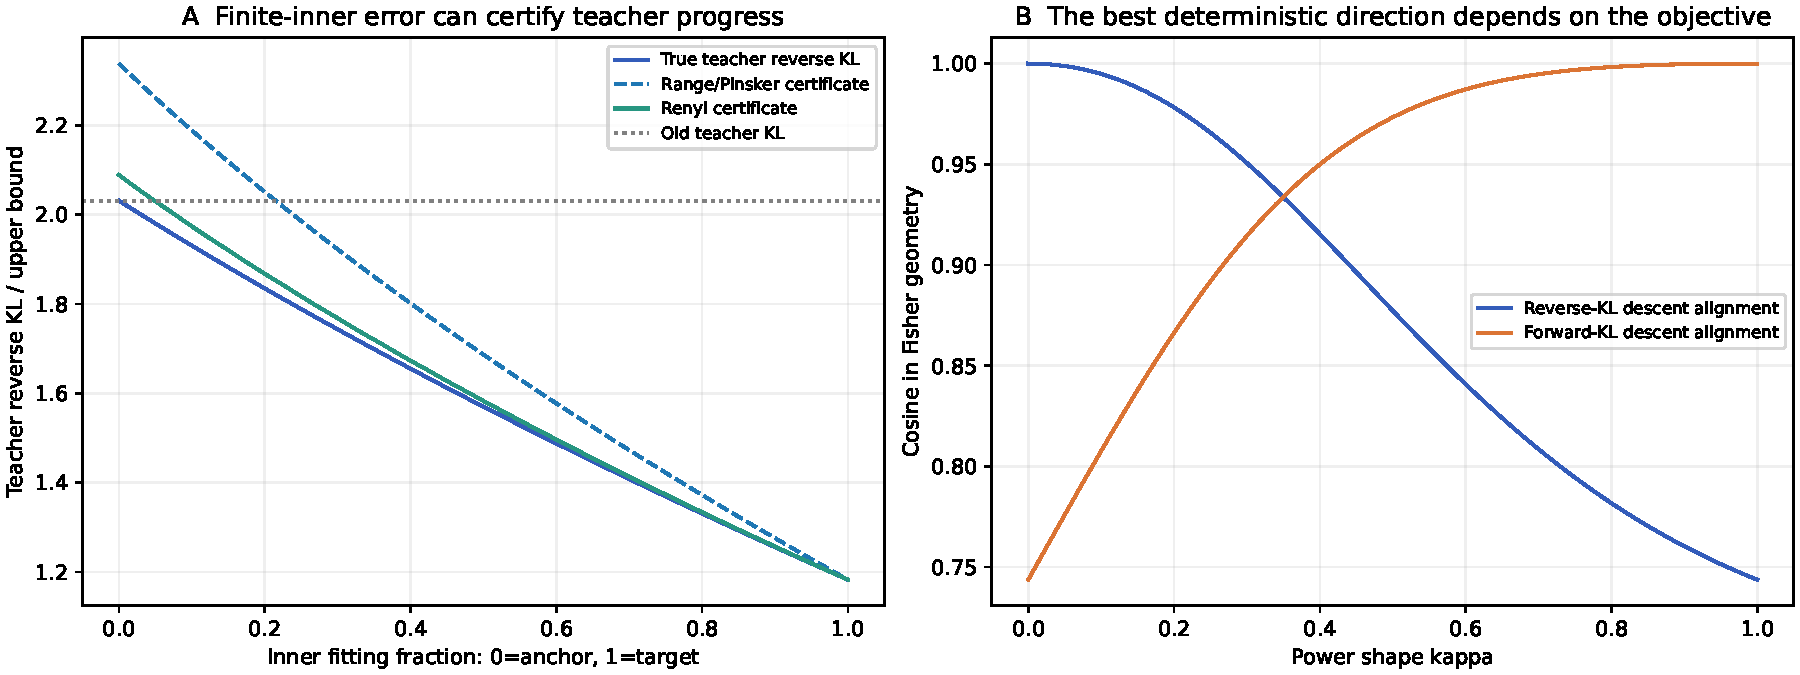
\includegraphics[width=\textwidth]{../../results/power-mean-20261013/inner-certificate-and-direction.pdf}
 \caption{左图将内层拟合误差转为 teacher reverse KL 的区间与 Rényi 上界；右图在相同 Fisher 速度下比较共同评价目标的方向。几何与算术分别对 reverse 与 forward KL 具有局部最陡性质。}
\end{figure}

本节的 Markov 核、半径单调性、有限 inner 证书与方向计算由 \path{experiments/analysis/power_generalization.py} 核验。大模型前缀、四卡训练与预注册判据见实验报告的幂均值部分；数学保证、真实 logit 协方差和实际全参数梯度分别报告。

\subsection{精确外层与有限 inner 的散度进展}

\begin{theorem}[teacher 散度的进展恒等式]
\label{thm:proximal-teacher-progress}
记 $c_\kappa=Z^\kappa$，端点 $\kappa=0,1$ 取 $c_\kappa=1$。对任意候选 $p$，有
\begin{equation}
 \eta\left[D_\kappa(T\Vert q)-D_\kappa(T\Vert p)\right]
 =(1-\eta)D_\kappa(q\Vert p)
 +c_\kappa\left[D_\kappa(m\Vert q)-D_\kappa(m\Vert p)\right].
 \label{eq:proximal-progress-identity}
\end{equation}
若 $D_\kappa(m\Vert p)\le D_\kappa(m\Vert q)$，则 teacher 散度不会增加。精确更新 $p=m$ 且 $q\ne T$ 时严格下降。
\end{theorem}

\begin{proof}
$F(q)=\eta D_\kappa(T\Vert q)$，而 $F(p)=(1-\eta)D_\kappa(q\Vert p)+\eta D_\kappa(T\Vert p)$。由定理~\ref{thm:proximal-barycenter-gap}，$F(q)-F(p)=c_\kappa[D_\kappa(m\Vert q)-D_\kappa(m\Vert p)]$。将 $F(q),F(p)$ 的定义代入并移项，即得恒等式。若目标散度改善，右侧两项非负；若 $p=m$、$q\ne T$，$m\ne q$，则至少第一项严格为正。最后，$m=q$ 会要求 $T_a^\kappa$ 与 $q_a^\kappa$ 成同一比例，概率归一化强制 $T=q$；两个端点同样成立。\hfill$\square$
\end{proof}

这给出了一个纯数学的 finite-inner 条件：降低本轮的 $D_\kappa(m\Vert p)$ 就能提高同一 $D_\kappa$ 下的 teacher 接近度。这里 teacher 散度的方向随 $\kappa$ 改变；一般 $\kappa$ 的保证不能直接替换成每步 $\KL(p\Vert T)$ 都下降。用其他拟合损失获得同一 target，只能在精确求解时自动继承本结论。
\subsection{escort 坐标中的线性轨迹与全局收敛}

对 $\kappa>0$ 定义 escort 分布和幂和
\begin{equation}
 E_\kappa(q)_a=\frac{q_a^\kappa}{S_\kappa(q)},\qquad
 S_\kappa(q)=\sum_aq_a^\kappa.
\end{equation}
$E_\kappa$ 是单纯形上的双射，逆映射为 $q_a\propto E_\kappa(q)_a^{1/\kappa}$。由 $m_a^\kappa=S_a/Z^\kappa$，共同的归一化因子在 escort 中消失，故
\begin{equation}
 E_\kappa(m)=(1-a^{\mathrm{esc}})E_\kappa(q)+a^{\mathrm{esc}}E_\kappa(T),\qquad
 a^{\mathrm{esc}}=\frac{\eta S_\kappa(T)}{(1-\eta)S_\kappa(q)+\eta S_\kappa(T)}.
 \label{eq:proximal-escort-step}
\end{equation}
这是精确式，不是局部近似。$\kappa=1$ 时 $S_1=1$，恢复 $a^{\mathrm{esc}}=\eta$；$0<\kappa<1$ 时，$S_\kappa(q)=\exp((1-\kappa)H_\kappa(q))$，其中 $H_\kappa$ 是 Rényi 熵。因此固定的概率幂插值强度在 escort 坐标中表现为随分布熵改变的有效步幅。

\begin{figure}[htbp]
 \centering
 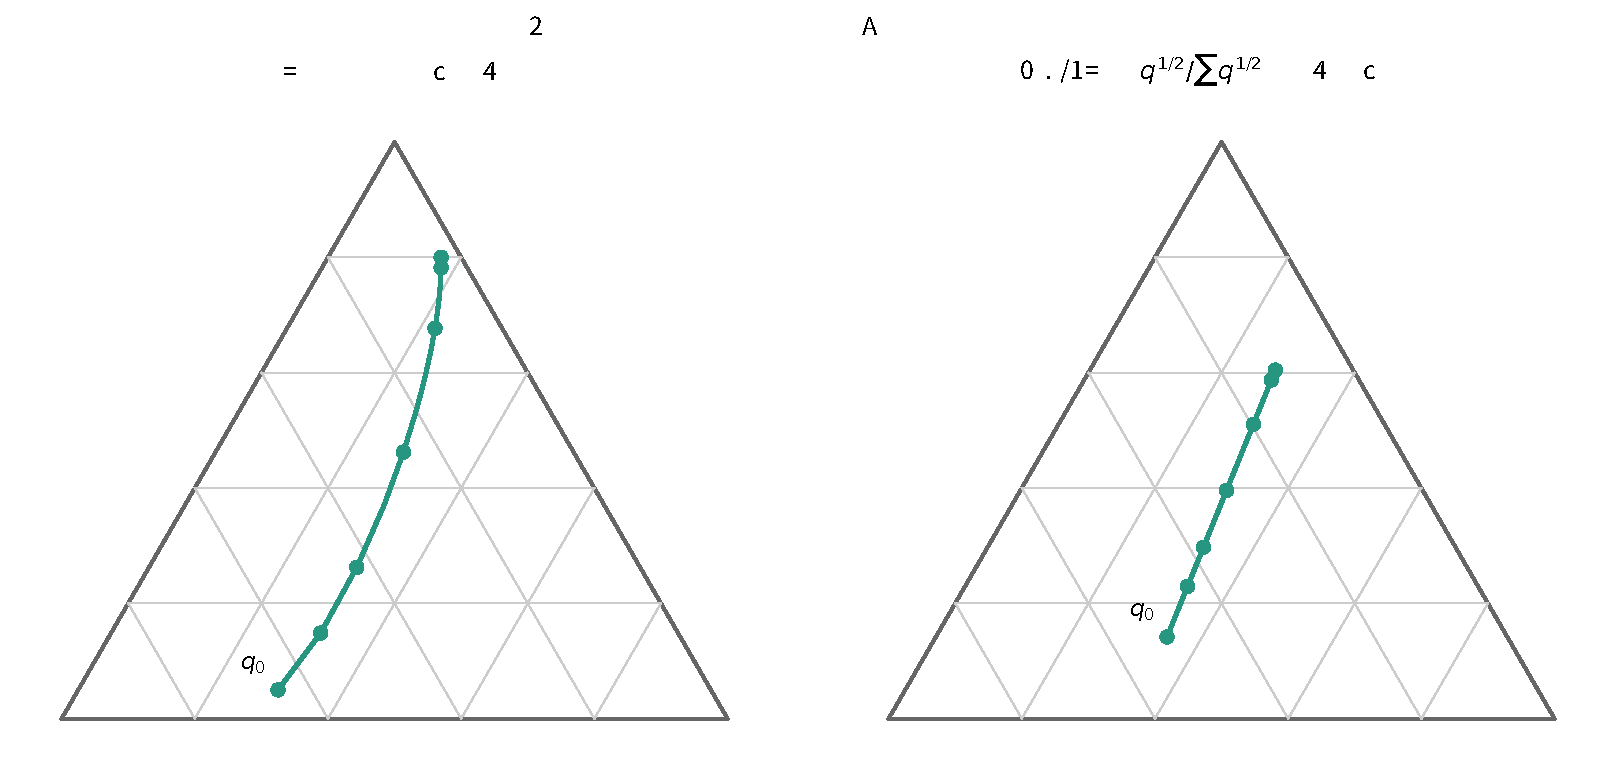
\includegraphics[width=\textwidth]{../../results/proximal-family-geometry/escort.pdf}
 \caption{同一平方根外层轨迹在概率坐标中弯曲，在 escort 坐标中是直线。圆点和数字表示迭代时点。高维分量在固定教师下共享一个进度系数。}
\end{figure}

若 $q_{n+1}=m_{\kappa,\eta}(q_n,T)$，记 $e_n=E_\kappa(q_n)$，则
\begin{equation}
 e_n-e_T=b_n(e_0-e_T),\qquad
 b_n=\prod_{j=0}^{n-1}(1-a_j^{\mathrm{esc}}).
 \label{eq:proximal-escort-orbit}
\end{equation}
这将固定教师下的 $d-1$ 维精确外层轨迹归结为一个标量 $b_n$。对连续自然梯度流，$dq_a/dt=q_a(\rho_a^\kappa-a_\kappa)/\kappa$，所以
\begin{align}
 \frac{d}{dt}q_a^\kappa&=T_a^\kappa-a_\kappa q_a^\kappa,\\
 \frac{d}{dt}S_\kappa(q)&=S_\kappa(T)-a_\kappa S_\kappa(q),\\
 \frac{d}{dt}E_\kappa(q)&=\frac{S_\kappa(T)}{S_\kappa(q)}[E_\kappa(T)-E_\kappa(q)].
\end{align}
改用时间 $\sigma$，$d\sigma/dt=S_\kappa(T)/S_\kappa(q)>0$，就有 $e(\sigma)=e_T+e^{-\sigma}(e_0-e_T)$。离散步式~\eqref{eq:proximal-escort-step} 也位于同一条流轨迹上，对应时间增量 $-\log(1-a^{\mathrm{esc}})$。精确幂均值步因此是这个自然梯度流轨迹的一种时间重参数化，而不只是具有相同起始切线。

\begin{theorem}[teacher 定向的 escort 收缩与误差累积]
\label{thm:proximal-escort-contraction}
令 $d$ 为词表大小，$0<\kappa\le1$，定义度量 $d_\kappa(q,T)=\|E_\kappa(q)-E_\kappa(T)\|_1$。对固定 teacher 的精确更新有
\begin{equation}
 d_\kappa(q_{n+1},T)=(1-a_n^{\mathrm{esc}})d_\kappa(q_n,T)\le c\,d_\kappa(q_n,T),\quad
 c=\frac{(1-\eta)d^{1-\kappa}}{(1-\eta)d^{1-\kappa}+\eta S_\kappa(T)}<1.
\end{equation}
故 $q_n\to T$。若近似更新满足 $d_\kappa(q_{n+1},m(q_n,T))\le\epsilon_n$，则
\begin{equation}
 d_\kappa(q_n,T)\le c^nd_\kappa(q_0,T)+\sum_{j=0}^{n-1}c^{n-1-j}\epsilon_j,
 \qquad
 \limsup_nd_\kappa(q_n,T)\le\frac{\epsilon_\infty}{1-c}
\end{equation}
其中最后一式要求 $\limsup_n\epsilon_n\le\epsilon_\infty$。
\end{theorem}

\begin{proof}
式~\eqref{eq:proximal-escort-step} 给出距离的精确比例。Jensen 不等式给出 $S_\kappa(q)\le d^{1-\kappa}$，因此 $1-a_n^{\mathrm{esc}}\le c$。反复应用得到精确更新的 $c^n$ 界；escort 逆映射连续，故 $q_n\to T$。近似更新时，三角不等式给出 $d_\kappa(q_{n+1},T)\le\epsilon_n+c\,d_\kappa(q_n,T)$，展开得到有限步式。对任意 $\delta>0$，取 $N$ 使 $j\ge N$ 时 $\epsilon_j\le\epsilon_\infty+\delta$。有限个早期项乘以 $c^{n-1-j}$ 后趋于零，后期项的和不超过 $(\epsilon_\infty+\delta)\sum_{i\ge0}c^i$。令 $\delta\to0$ 得极限上界。\hfill$\square$
\end{proof}

这是对固定 teacher 的定向收缩，不声称两个任意 anchor 经同一算子后具有同一个收缩系数；它也不直接等于原概率空间的 TV 收缩。$\kappa\to0$ 时，escort 本身趋于均匀分布，必须重标度才保留信息：
\begin{equation}
 \frac d\kappa\left[E_\kappa(q)_a-\frac1d\right]
 \longrightarrow\log q_a-\frac1d\sum_b\log q_b.
\end{equation}
几何端点就在这些中心化 log 坐标中满足精确比例 $1-\eta$。在任何固定完整支持的 teacher 附近，所有 $\kappa$ 都有 $m(T+\delta,T)=T+(1-\eta)\delta+O(\|\delta\|^2)$，因为 $a_n^{\mathrm{esc}}\to\eta$。它们共享局部收敛率，远处的度量和有效时间则不同。

\begin{figure}[htbp]
 \centering
 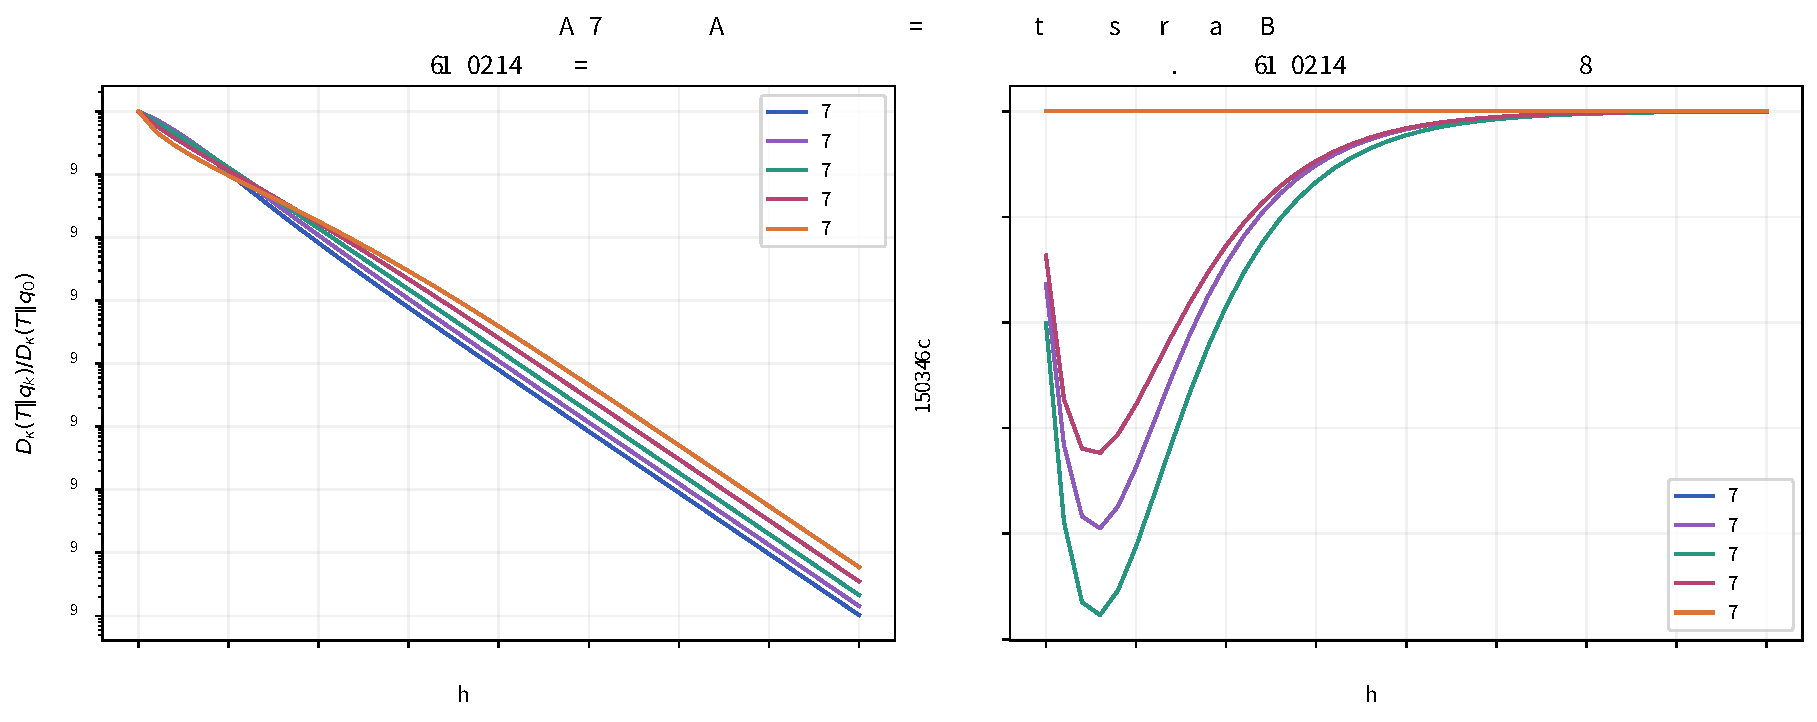
\includegraphics[width=\textwidth]{../../results/proximal-family-geometry/convergence.pdf}
 \caption{精确外层的 teacher 散度单调下降，有效 escort 步幅趋于共同的 $\eta$。每条曲线使用各自的 $D_\kappa$ 并按初值归一化，图中的高低不能直接作为同一任务的训练性能排名。}
\end{figure}
\subsection{共享参数子流形上的自然梯度投影}

独立 token 分布的速度界还可延伸到共享参数的自然梯度流，但需要明确度量。取有限个 prefix、固定权重 $d_s>0$、$\sum_sd_s=1$，将外层分布写成 $q_\theta(a\mid s)>0$。定义
\begin{equation}
 L_\kappa(\theta)=\sum_sd_sD_\kappa(T_s\Vert q_{\theta,s}),\qquad
 \langle v,w\rangle_W=\sum_{s,a}\frac{d_s}{q_{\theta,s,a}}v_{s,a}w_{s,a}.
\end{equation}
记 $J=\partial q_\theta/\partial\theta$，$W=\operatorname{diag}(d_s/q_{\theta,s,a})$，则参数 Fisher 矩阵为 $\mathcal I=J^\top WJ$。令 $v$ 为每个 prefix 上的无约束负自然梯度，$v_{s,a}=q_{\theta,s,a}(\rho_{s,a}^\kappa-\E_{q_{\theta,s}}\rho_s^\kappa)/\kappa$。因为每个 prefix 的 $J$ 列向量分量和为零，$\nabla_\theta L=-J^\top Wv$。

参数自然梯度流采用 Moore--Penrose 广义逆 $\mathcal I^+$ 时，有
\begin{equation}
 \dot\theta=-\mathcal I^+\nabla_\theta L,\qquad
 \dot q_\theta=J\mathcal I^+J^\top Wv=Pv.
\end{equation}
$P$ 是到 $\operatorname{range}(J)$ 的 $W$ 正交投影：令 $B=W^{1/2}J$，则 $W^{1/2}PW^{-1/2}=B(B^\top B)^+B^\top$，后者是普通欧氏正交投影。因此
\begin{equation}
 \|\dot q_\theta\|_W^2\le\|v\|_W^2,\qquad
 \frac{dL}{dt}=-\langle v,Pv\rangle_W=-\|Pv\|_W^2\le0.
\end{equation}
平方根形状满足 $\|v\|_W^2=\sum_sd_s\,4(1-a_s^2)\le4$，所以共享参数的精确自然梯度流也满足 $\|\dot q_\theta\|_W\le2$。更一般地，$0<\kappa\le1/2$ 时平方速度不超过 $1/\kappa^2$。

这个结论控制的是分布流在固定 prefix Fisher 度量下的速度。它不控制参数的欧氏范数，也不自动适用于普通梯度流。共享参数还可能使 $Pv=0$ 而 $q_\theta\ne T$，因此单调性和速度界并不保证无投影误差的 teacher 收敛。离散幂均值 target 的精确 escort 轨迹也不会因这个局部投影结论自动延续到共享参数模型。

\subsection{target 形状与拟合形状是两个参数}

前文 $\kappa$ 用于构造 $m_{\kappa,\eta}$，本小节明确写为 $\kappa_{\mathrm{target}}$。拟合一个已经冻结的 $m$ 时，可以另外选择 $\kappa_{\mathrm{fit}}$，最小化 $D_{\kappa_{\mathrm{fit}}}(m\Vert p)$。前文的重心进展恒等式直接对应两者相等的情形；两者不相等时仍共享最优点 $p=m$，但有限 inner 应使用 reverse KL/Rényi 证书或另行证明共同评价目标的进展。

因此，几何 target 可以搭配 Hellinger 拟合，算术 target 也可以搭配 Hellinger 拟合。下面的最优常数结论作用于拟合形状，不能直接宣称平方根 target 对任何任务都最优。

\subsection{当前学生采样的误差相关梯度矩界}

固定 prefix 和 target $m$，本小节记 $k=\kappa_{\mathrm{fit}}$。从当前学生 $a\sim p$ 采样动作，令 $\chi=m/p$、$a_k=\E_p\chi^k$、$\psi_p=\nabla_\theta\log p$。解析微分 $D_k(m\Vert p)$，并利用 $\E_p\psi_p=0$，得到无偏估计量
\begin{equation}
 g_k(a)=\frac{a_k-\chi_a^k}{k}\psi_p(a),\qquad
 \E_pg_k=\nabla_\theta D_k(m\Vert p).
\end{equation}
它在 $p=m$ 时逐 action 为零。前缀保持固定、动作从当前学生重采样，与每步重新生成完整 response 是两种不同的测度操作。

\begin{theorem}[误差相关二阶矩的锐常数]
\label{thm:proximal-sharp-self-bound}
若 $\|\psi_p(a)\|\le S$、$0<k\le1/2$，则
\begin{equation}
 \Var_p(g_k)\le\E_p\|g_k\|^2
 \le\frac{S^2}{k}D_k(m\Vert p).
\end{equation}
系数 $1/k$ 是对所有完整支持概率分布统一成立的锐常数。$k=0$ 或 $k>1/2$ 没有有限的统一误差相关常数。按此标准，$k=1/2$ 是该规范化散度族中的唯一最佳形状。
\end{theorem}

\begin{proof}
令 $a(u)=\E_p\chi^u$，则 $a(1)=1$，$a$ 对 $u$ 凸，且 $a(k)\le1$。由于 $2k\in[k,1]$，凸性给出
\begin{equation}
 a(2k)\le\frac{1-2k}{1-k}a(k)+\frac{k}{1-k}.
\end{equation}
所以
\begin{align}
 \Var_p(\chi^k)&=a(2k)-a(k)^2\\
 &\le\frac{(1-a(k))[k+(1-k)a(k)]}{1-k}\\
 &\le\frac{1-a(k)}{1-k}.
\end{align}
再由 $D_k(m\Vert p)=(1-a(k))/[k(1-k)]$，得到 $\E_p[(a_k-\chi^k)^2/k^2]\le D_k/k$，乘以 score 范数界即可。

为证明锐性，取 $p=(v,1-v)$、$m=(v^2,1-v^2)$，$v\to0$。比率为 $\chi=(v,1+v)$，因此 $a(k)=1-(1-k)v+o(v)$、$a(2k)=1-(1-2k)v+o(v)$，有 $\Var_p\chi^k=v+o(v)$、$D_k=v/k+o(v)$。系数二阶矩与损失之比趋于 $1/k$。categorical logits 的 rare-action score 范数平方趋于 2，其概率为 $v$，common-action score 范数平方为 $O(v^2)$，故实际梯度二阶矩也达到这个相对常数；均值平方为 $O(v^2)$，方差具有同一极限。

$1/2<k<1$ 时，取 $p=(v,1-v)$、$m=(1/2,1/2)$，系数方差按 $v^{1-2k}$ 发散，但 $D_k\le1/[k(1-k)]$。$k=1$ 时系数方差按 $1/v$ 发散，损失只按 $\log(1/v)$ 增长。$k=0$ 的 centred log-ratio 系数二阶矩可按 $\log^2(1/m_a)$ 增长，而 reverse KL 只按 $\log(1/m_a)$ 增长。取非对称、固定正质量的学生即可使梯度方差与损失的比也发散。\hfill$\square$
\end{proof}

在平方根点，这个关系更精确：$a=\sum\sqrt{pm}$，$D_{1/2}=4(1-a)$，系数二阶矩为 $4(1-a^2)=D_{1/2}(1+a)$。它既有统一绝对上界 4，也随拟合误差消失。若使用损失 $L=D_{1/2}/\eta$，对应的缩放梯度满足 $\E\|g/\eta\|^2\le(2S^2/\eta)L$。模型投影误差不为零时，这个结论不强制噪声消失。

\subsection{精确 BPO 已有残差驱动的噪声控制}

对任意 target $m$ 与冻结 anchor $q$，定义 $R=C_q\log(p/m)$ 和 $L_{\mathrm{BPO}}=\E_qR^2/(2\eta)$。解析梯度中 centre 的导数乘以 $\E_qR=0$ 后消失，因此 $g=R\psi_p/\eta$ 是 anchor 动作采样的无偏估计量，并满足
\begin{equation}
 \E_q\|g\|^2\le\frac{S^2}{\eta^2}\E_qR^2
 =\frac{2S^2}{\eta}L_{\mathrm{BPO}}.
\end{equation}
所以误差相关的噪声控制不只存在于 Hellinger 拟合；BPO 本来就具有这项性质。区别是 BPO 残差损失可任意大，而 Hellinger 损失不超过 4。几何 target 的初始 BPO 误差仍可能由极端 teacher log-ratio 主导；改变 target 的形状可以控制这个初始误差。生产 Top-$J$ centre 与完整词表条件均值之间的偏差，必须与这个精确结论区分。

\subsection{平方根 target 和平方根拟合的初始矩界}

若 $m=m_{1/2,\eta}(q,T)$，令 $a=\sum\sqrt{qT}$、$Z=(1-\eta)^2+\eta^2+2\eta(1-\eta)a$。在 inner 起点 $p=q$，有
\begin{equation}
 \sum_a\sqrt{q_am_a}=\frac{1-\eta+\eta a}{\sqrt Z},\qquad
 1-\left(\sum_a\sqrt{q_am_a}\right)^2=\frac{\eta^2(1-a^2)}Z.
\end{equation}
因此平方根拟合的梯度系数在除以 $\eta$ 后，二阶矩为 $4(1-a^2)/Z\le4/[(1-\eta)^2+\eta^2]\le8$。这给出同时对所有 teacher、anchor 和 $0<\eta<1$ 成立的初始上界；其 Fisher--Rao 目标位移也由相同的角度恒等式控制。这个干净的联合性质支持研究平方根组合，但不等于所有数据上的最高信噪比或最佳任务成绩。

\subsection{局部 SGD 收敛与投影误差的条件结论}

\begin{theorem}[误差相关噪声下的条件 SGD 收敛]
\label{thm:power-conditional-sgd}
固定前缀测度，设最小投影损失为 $L_\star\ge0$。假设所有随机更新线段所在区域中 $L$ 为 $L_{\mathrm{sm}}$ 光滑，满足 Polyak--\L{}ojasiewicz（PL）条件 $\|\nabla L\|^2\ge2\mu(L-L_\star)$，且当前参数固定后的估计量满足 $\E[g\mid\theta]=\nabla L$、$\E[\|g\|^2\mid\theta]\le CL$。固定
\begin{equation}
 0<\alpha_{\mathrm{opt}}\le\min\{1/\mu,2\mu/(L_{\mathrm{sm}}C)\},\qquad
 c_{\mathrm{SGD}}=1-\mu\alpha_{\mathrm{opt}}\in[0,1).
\end{equation}
则 SGD 迭代满足
\begin{equation}
 \E[L(\theta_N)-L_\star]
 \le c_{\mathrm{SGD}}^N[L(\theta_0)-L_\star]
 +\frac{L_{\mathrm{sm}}C\alpha_{\mathrm{opt}}L_\star}{2\mu}(1-c_{\mathrm{SGD}}^N).
\end{equation}
目标可实现且 $L_\star=0$ 时，残差驱动的采样噪声不产生固定步长误差底；$L_\star>0$ 时上式明确给出投影误差对应的噪声项。
\end{theorem}

\begin{proof}
令 $\theta^+=\theta-\alpha_{\mathrm{opt}}g$。光滑性、无偏性和二阶矩界给出
\begin{align}
 \E[L(\theta^+)\mid\theta]
 &\le L-\alpha_{\mathrm{opt}}\|\nabla L\|^2+
 \frac{L_{\mathrm{sm}}\alpha_{\mathrm{opt}}^2}2\E\|g\|^2\\
 &\le L-2\mu\alpha_{\mathrm{opt}}(L-L_\star)
 +\frac{L_{\mathrm{sm}}C\alpha_{\mathrm{opt}}^2}{2}L.
\end{align}
将 $L=(L-L_\star)+L_\star$ 代入，再使用 $L_{\mathrm{sm}}C\alpha_{\mathrm{opt}}^2/2\le\mu\alpha_{\mathrm{opt}}$，得到
\begin{equation}
 \E[L(\theta^+)-L_\star\mid\theta]
 \le c_{\mathrm{SGD}}(L-L_\star)+L_{\mathrm{sm}}C\alpha_{\mathrm{opt}}^2L_\star/2.
\end{equation}
对全体历史求期望，递推 $N$ 次并使用 $\sum_{j=0}^{N-1}c_{\mathrm{SGD}}^j=(1-c_{\mathrm{SGD}}^N)/(\mu\alpha_{\mathrm{opt}})$，得到结论。
\end{proof}

这些是带明确光滑性、PL、可实现性和 score 条件的 SGD 结论。共享参数模型与实际优化器需要分别核实这些假设；条件 SGD 定理不能直接作为大模型训练的保证。

\subsection{同一重心恒等式的多分布扩展}

多个固定分布 $T^{(j)}$、权重 $w_j\ge0$、$\sum_jw_j=1$ 时，同一证明给出
\begin{equation}
 \argmin_p\sum_jw_jD_\kappa(T^{(j)}\Vert p)
 \propto\left[\sum_jw_j(T^{(j)})^\kappa\right]^{1/\kappa}.
\end{equation}
完整支持下，几何、平方根与算术的多教师汇合均在同一框架内；可将 anchor 作为其中一个分布。超额损失分解及最优点的 Fisher 曲率也直接延续。


\section{序列边界与可用性质}
\label{sec:power-scope}
\subsection{条件分布的改善与完整轨迹的改善}

在固定长度 $H$ 的 autoregressive 模型中，记完整序列分布为 $Q(y)=\prod_iq(y_i\mid y_{<i})$、$T(y)=\prod_it(y_i\mid y_{<i})$。KL 链式法则给出
\begin{equation}
 \KL(Q\Vert T)=\sum_{i=1}^H\E_{s_i\sim Q}\KL(q(\cdot\mid s_i)\Vert T(\cdot\mid s_i)).
 \label{eq:proximal-sequence-chain}
\end{equation}
更新每个条件分布后，访问测度也从 $Q$ 变成 $P$。因此逐个 prefix 的条件 KL 下降，不足以让这条随策略改变权重的总和下降。本书固定测度问题明确冻结权重；序列混合与逐 token 混合是不同算子。

\paragraph{一个两步、完整支持的反例。}
第一步取 $q_0=(0.99,0.01)$、$T_0=(0.01,0.99)$。第一分支的第二步取 $q_A=T_A=(1/2,1/2)$；第二分支取 $q_B=(1-10^{-6},10^{-6})$、$T_B=(10^{-30},1-10^{-30})$。在全部三个条件分布上同时执行精确幂均值步，$\eta=0.1$。每个条件 KL 都下降或保持零，但完整序列的 reverse KL 为
\begin{center}
\begin{tabular}{lrr}
\toprule
形状 & 更新前完整序列 KL & 更新后完整序列 KL\\
\midrule
$\kappa=0$ & 5.19399 & 6.07445\\
$\kappa=1/2$ & 5.19399 & 7.09792\\
$\kappa=1$ & 5.19399 & 10.44581\\
\bottomrule
\end{tabular}
\end{center}
数值由 \path{results/power-mean-20261013/generalization-checks.json} 的完整精度记录为准。变化的原因是学生更频繁进入尚未拟合好的第二分支。算术形状将该分支概率从 $0.01$ 提升到 $0.108$，其条件误差仍然很大。保持原访问权重的条件 KL 总和却从 $5.19399$ 降到 $4.38503$；两种测度给出不同结论。这个反例在固定两步时域已成立，不依赖 EOS 或长度归一化。

\begin{figure}[htbp]
 \centering
 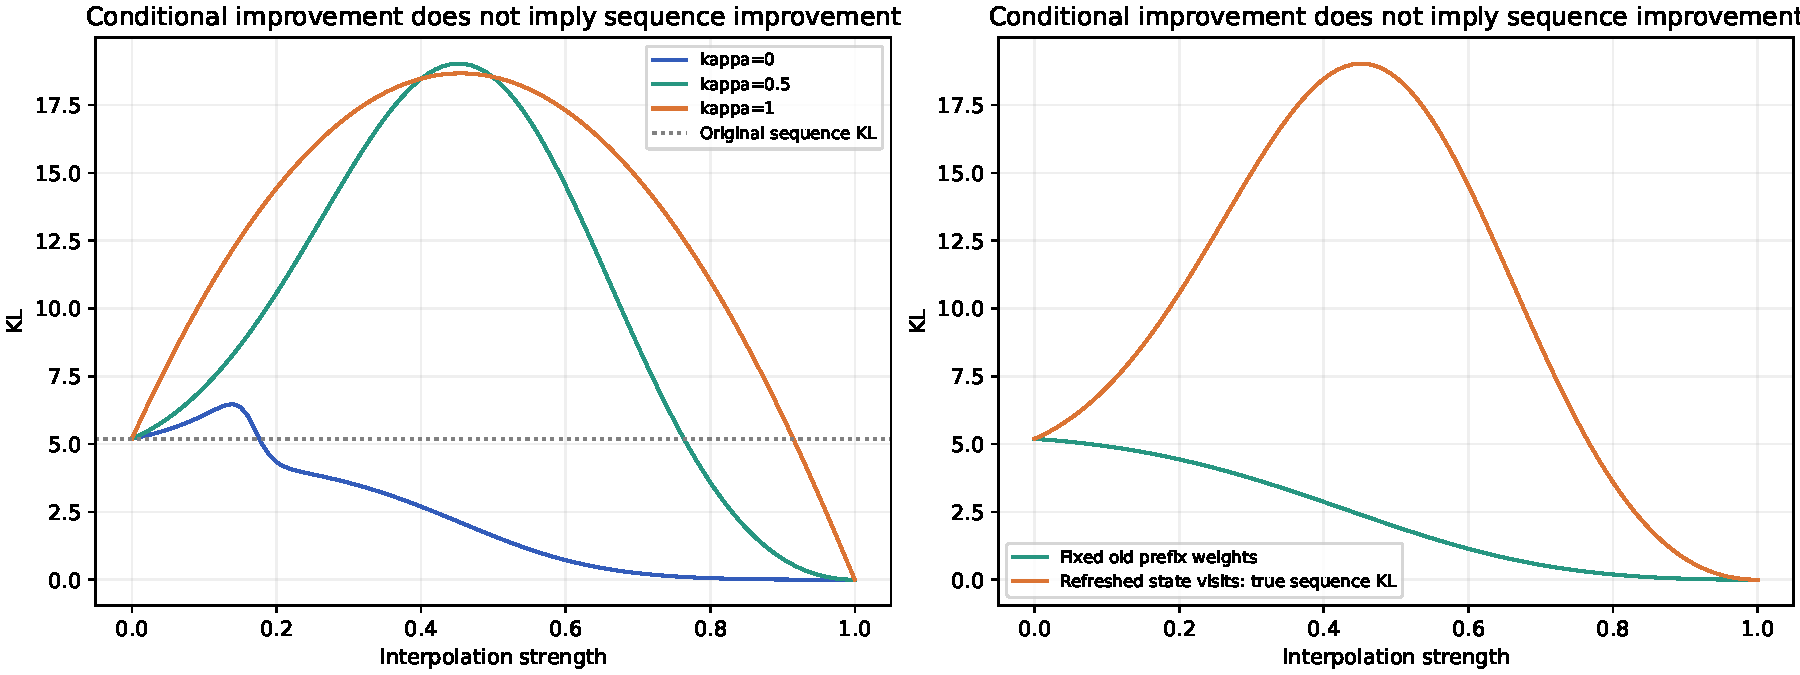
\includegraphics[width=\textwidth]{../../results/power-mean-20261013/sequence-scope-counterexample.pdf}
 \caption{精确条件更新仍可能使完整序列 KL 上升。左图比较三种形状；右图固定平方根形状，对照冻结旧 prefix 权重的条件目标与更新后访问测度下的真实序列 KL。}
\end{figure}

\subsection{序列混合的条件概率包含额外因子}

对序列层面的算术混合 $M=(1-\eta)Q+\eta T$，条件分布为
\begin{equation}
 M(a\mid s)=(1-\eta_s)q(a\mid s)+\eta_st(a\mid s),\qquad
 \eta_s=\frac{\eta T(s)}{(1-\eta)Q(s)+\eta T(s)}.
\end{equation}
它的 teacher 权重依赖已经生成的 prefix。固定 $\eta$ 的逐 token 算术混合因此一般不同于序列层面的算术混合。

对序列几何 target $M(y)\propto Q(y)^{1-\eta}T(y)^\eta$，定义后缀配分函数
\begin{equation}
 Z_\eta(s)=\sum_zQ(z\mid s)^{1-\eta}T(z\mid s)^\eta.
\end{equation}
将带前缀 $s$ 的序列质量先求和再作条件化，得到
\begin{equation}
 M(a\mid s)=q(a\mid s)^{1-\eta}T(a\mid s)^\eta
 \frac{Z_\eta(sa)}{Z_\eta(s)}.
\end{equation}
逐 token 几何 target 忽略了 action 相关的后缀配分函数；它只有在这些后缀因子与 action 无关时才恢复完整序列 target。两个端点都展示了条件化与混合一般不能交换。

\subsection{真实序列 reverse KL 的一阶方向}

记 suffix 值 $V^q(s)=\KL(Q(\cdot\mid s)\Vert T(\cdot\mid s))$。链式法则给出递推
\begin{equation}
 V^q(s)=\E_{a\sim q(\cdot\mid s)}[\log(q(a\mid s)/T(a\mid s))+V^q(sa)],
\end{equation}
终点的值为零。完整序列 KL 的 policy gradient 是
\begin{equation}
 \nabla\KL(Q\Vert T)
 =\E_Q\sum_i\psi_i\sum_{j\ge i}\log\frac{q(y_j\mid s_j)}{T(y_j\mid s_j)}.
\end{equation}
推导时，$\nabla\log Q=\sum_i\psi_i$，直接微分 KL 多出的 $\E_Q\nabla\log Q$ 为零；过去 reward 与当前 score 的乘积则因条件零均值而消失。对某个 prefix 的局部方向，未来成本不能省略；其负信号是
\begin{equation}
 f_{\mathrm{seq}}^q(s,a)=\log\frac{T(a\mid s)}{q(a\mid s)}-V^q(sa).
\end{equation}
条件中心化后，它给出真实序列 reverse KL 的自然梯度方向。即时 log-ratio 的固定测度优化只保留第一项。长度平均的未来 return、随机组标准化或其他信号变换需要另行解释其目标，不能直接继承这条精确 policy gradient。

若直接在有限序列空间构造幂均值 target，前面的凸生成散度与矩定理仍然成立。该空间虽有指数级的序列数，归一化的二阶矩界不含空间大小。若每个 token score 范数不超过 $S$，$H$ 有限，则序列 score 范数不超过 $HS$，对应的梯度二阶矩界只增加 $H^2S^2$ 因子。序列 target 的表达、采样和投影是不同问题；固定 prefix 理论与任务正确率是不同证据，须分别报告。

\subsection{固定条件问题中可以直接使用的性质}

单教师的幂均值框架提供了三个相互连接的保证。正形状 $\kappa>0$ 改变极端教师概率比的尾部；固定 $(\kappa,\eta)$ 的精确更新下降一个明确的有界教师目标 $\mathcal J$；$0<\kappa\le1/2$ 的中心化监督方差又由中心 $K$ 控制。BPO 拟合的残差采样梯度随其损失下降而消失，形状变换与残差回归分别控制初始监督和拟合末期的噪声。

\begin{center}
\small
\begin{tabular}{p{46mm}p{54mm}p{45mm}}
\toprule
可用性质 & 必要条件 & 实际含义\\
\midrule
精确 target 同时改善全部凸 $f$ 散度 & 同一固定 teacher、完整正支持 & 同一评价量下可比较不同形状\\
教师覆盖与刷新后的双侧监督界 & $\kappa>0$，同一前缀精确刷新 & $q_n\ge\eta^{1/\kappa}T$，控制未来正尾部\\
精确 MD 下降与最后迭代界 & 固定 $\kappa,\eta$，每步刷新锚点 & $\mathcal J(q_N)\le\KL(T\Vert q_0)/(\eta N)$\\
教师监督方差受误差控制且可求和 & $0<\kappa\le1/2$，精确外层 & 教师接近度与监督噪声共同趋零\\
BPO 的零残差零采样梯度 & target 可实现、精确中心或无偏差分损失 & 避免固定中心误差造成的噪声底\\
有限 inner 的全部 teacher 散度进展 & 从 $q$ 出发的指定 Fisher 预条件路径 & 实际任意 BPO loss 下降不充分\\
有界中心估计与可认证尾部误差 & 已知 $q,T$ 概率或所需尾部查询接口 & 不增加 response 数仍可估计中心\\
\bottomrule
\end{tabular}
\end{center}

以上几何重心与球面性质属于已有信息几何框架；本章不据此宣称研究新颖性。本章用于 MirrorOPD 的增量在于明确分开重心、有限步 MD 目标、BPO 投影和估计器，并把它们连接为条件进展与噪声界。任务表现仍受共享参数、不可实现 target、有限 inner 和前缀访问变化影响。理论上可证明的对象与需要实测的对象在表中分别列出。

\subsection{原始几何信号的尺度与标准化反例}

在前八章的归一化下，记 $r=\log(T/q)$、$U=\log(p/q)$、$\psi=\nabla\log p$，三个原始下降方向为
\begin{align}
 -\nabla\mathcal L_{\mathrm{Mean}}&=\E_q[(\eta C_qr-U)\psi],\\
 -\nabla\mathcal L_{\mathrm{BPO}}&=\E_q[(C_qr-C_qU/\eta)\psi],\\
 -\nabla\mathcal L_{\mathrm{MDPO}}&=\E_p[(r-U/\eta)\psi].
\end{align}
在 $p=q$ 时，PMD-Mean 起始梯度带整体 $\eta$，BPO 与 MDPO 不带。第~\ref{sec:power-setup}~节二元反例中，未中心化的 MDPO 单点估计还满足
\begin{equation}
 \Var_q(\psi r)=v(1-v)[(1-v)r_1+vr_2]^2\longrightarrow\infty.
\end{equation}
这些尺度差异由具体损失归一化决定，不能仅由 target 的插值权重推断。

对二元信号 $f$，条件标准差为 $\sigma_f^2=v(1-v)(f_1-f_2)^2$。只要 $f_1\ne f_2$，逐 action 展开可得
\begin{equation}
 \Var_q[\psi C_qf/\sigma_f]=(1-2v)^2.
\end{equation}
单调信号变换在这个例子中被标准差缩放抵消。当前算法不使用这类随机标准差归一化；该反例用于限定原始方差界的适用对象。

\begin{figure}[htbp]
 \centering
 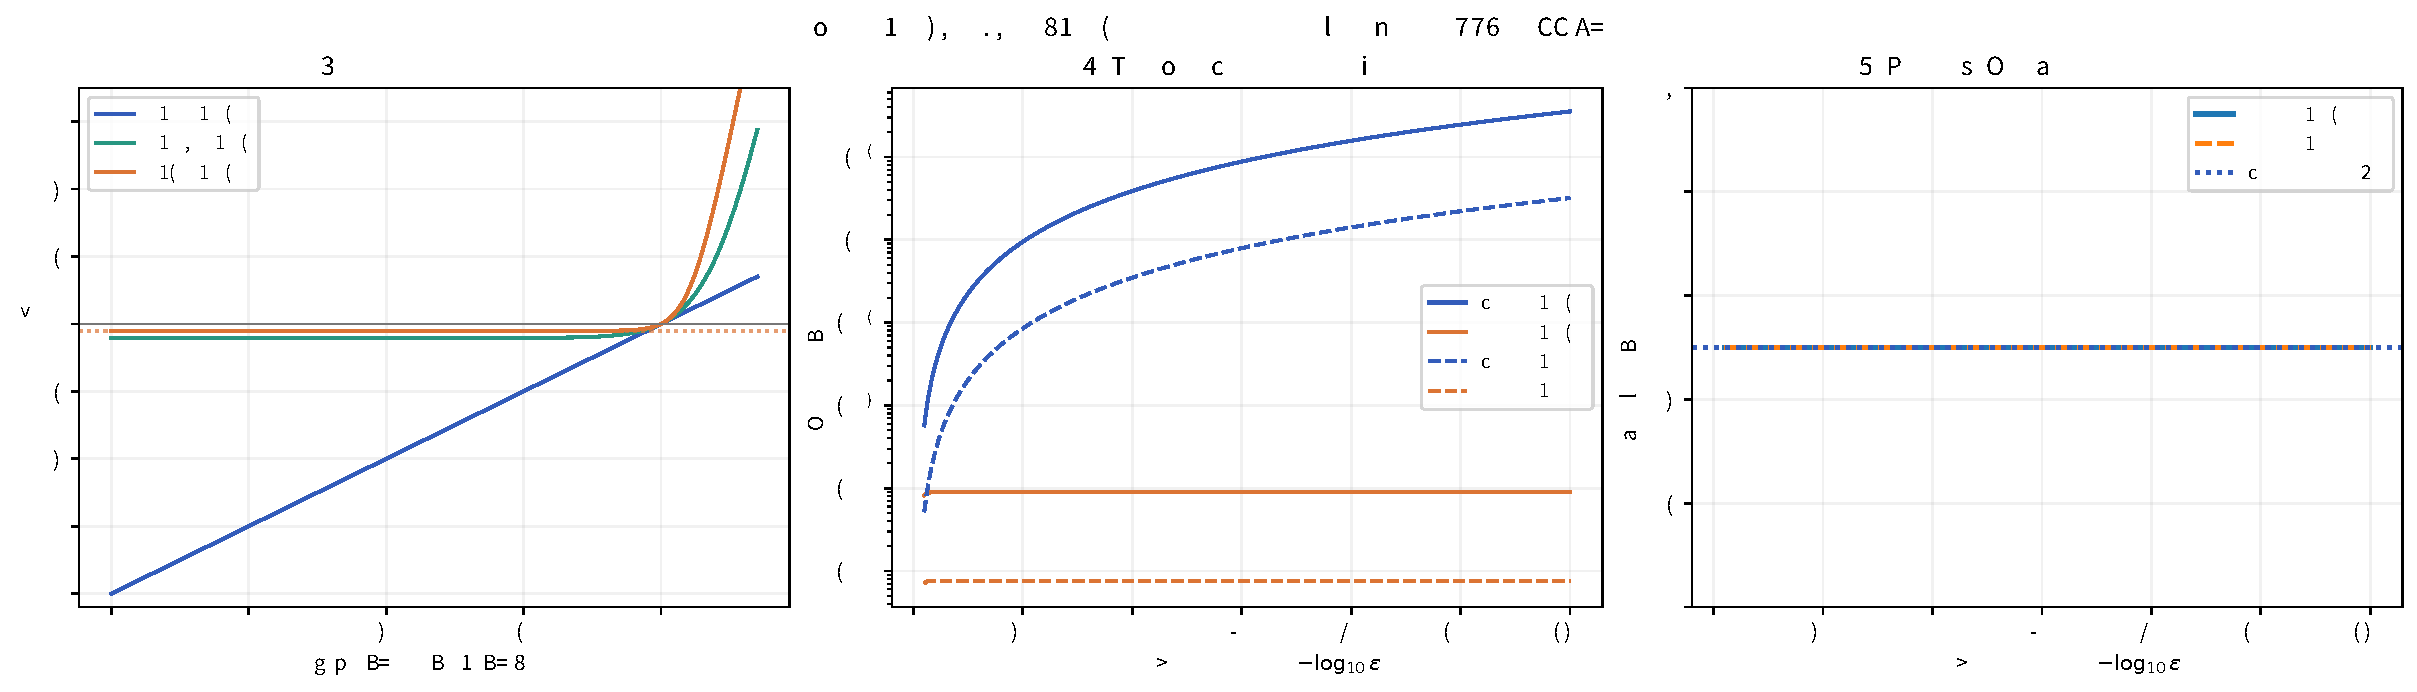
\includegraphics[width=\textwidth]{../../results/proximal-family-geometry/variance.pdf}
 \caption{尺度、尾部与标准化分别改变不同对象。早期图中 $\lambda$ 对应本章 $\eta$；中图使用 $q=(1/4,3/4)$ 的精确条件中心化 score 方差，右图验证二元标准差缩放的抵消现象。}
\end{figure}

\subsection{证明、解析图与实验记录的维护位置}

本章的图来自解析有限词表公式、已有模型缓存或已经登记的实验；正文与图注明确区分这些证据。重构只增加解析形状与反例图，不启动新的 GPU 训练。主线的 source、figure metadata 和确定性数值核验分别保存在 \path{docs/book/}、\path{results/chapter9-restructure/} 与对应第一方程序中。

原有几何、动力学和共享参数核验由 \path{experiments/analysis/proximal_family_geometry.py}、\path{experiments/analysis/proximal_family_dynamics.py} 生成。散度证书由 \path{experiments/analysis/power_generalization.py} 核验。中心和辅助采样的缓存审计位于 \path{results/power-center-advantage/} 与 \path{results/power-center-extensions/}。实际大模型 setting、结果和分析继续进入唯一实验报告，本章不复制待执行的 GPU 队列和运行流水。

